% !TeX root = ../main.tex

\chapter{Week Coupling (Canonical) Perturbation Theory}

Starting from the equation of motion of the Green's function
\begin{equation}
  \iu\pdif t G_\epsilon [\underset{s_i^+}{c_i}, \underset{s_j^-}{c_j^\dagger}]
= \delta_{ij}
\end{equation}
where the canonical means that the RHS is a $\delta$-function,
and $[s_i^+, s_j^-] = 2s_i^z\delta_{ij}$.
the operators satisfiy Wick's Theorem
\[
  \{c_i, c_j^\dagger\} = \delta_{ij}, \quad [a_i, a_j^\dagger] = \delta_ij
\]

\section{Wick Theorem}

For Gell-Mann-Low, the limitation
\[
  \lim_{\alpha\to0} \frac{u_\alpha^D(0,-\infty)\ket|\eta_0>}
    {\braket<\eta_0|u_\alpha^D(0,-\infty)|\eta_0>}
= \lim_{\alpha\to0} \frac{\ket|\Psi_\alpha^D(0)>}
    {\braket<\eta_0|\Psi_\alpha^D(0)>}
= 
\]
we can convert to the obverse $\braket<A^\text H(t)>$ by computing from the
GML theory
\begin{multline}
  \braket<E_0|A^\text H(t)|E_0>
= \lim_{\alpha\to0} \frac1{\braket<\eta_0|S_\alpha|\eta_0>}
  \sum_{n=0}^\infty \frac1{2^nn!}
  \ab(-\frac\iu\hbar)^n \upe^{-\alpha(|t_1|+\cdots+|t_n|)} \\ \times
  \int_{-\infty}^\infty \d t_1 \cdots \d t_n
  \braket<\eta_0|T_\epsilon
  \ab\{\hat V(t_1)\hat V(t_2) \cdots \hat V(t_n) A^\text H(t)\}|\eta_0>
\end{multline}
where
\[
  V = \frac12 \sum_{\substack{\alpha\beta\\\gamma\delta}}
    \braket<\alpha\beta|\hat V|\gamma\delta>
    a_\alpha^\dagger a_\beta^\dagger a_\gamma a_\delta
\]
The obverse
\[
  \braket<\alpha\beta|\hat V\gamma\delta>
= \braket<\beta\alpha|\hat V|\delta\gamma>
\]
For any observables
\[
  \braket<E_0|A(t) B(t^*) \cdots |E_0>
\]
which can be converted to
\[
  \cdots \int_{-\infty}^\infty \d t_1 \cdots \d t_n
  \braket<\eta_0|
  T_\epsilon\{V(t_1) \cdots V(t_n)
    \underset{a_i(t_i)}A(t) \underset{a_f^\dagger(t_f)}{B(t')} \cdots\}|\eta_0>
\]
To calculate it, consider
\[
  T_\epsilon(O_1(t_1)O_2(t_2)O_3(t_3)O_4(t_4))
\]
which has the order number $4! = 24$.

\section{Normal product}

The ``book-keeping'' of counting:
For a given $\ket|\eta_0>$, the fermi wave vector $k_F$, then
\[
  \gamma_k = \begin{cases}
    c_k^\dagger \ket|\eta_0> = 0, & |k| < k_F\\
    c_k \ket|\eta_0> = 0, & |k| > k_F
  \end{cases}
\]
where $\gamma_k\ket|\eta_0> = 0$.
Also for $\gamma_k^\dagger\ket|\eta_0>$.

For $N$-ordering: If we have an arbitrary sequence
\[
  N(\gamma_1 \gamma_2^\dagger \cdots \gamma_n)
  \to (\gamma^+\gamma^+ \cdots | \gamma \gamma \gamma)
\]
where some of the $\gamma$s have $\dagger$.
The normal ordering operator $N$ brings the $\dagger$ to the front.
\[
  \braket<\eta_0|N(\cdots) |\eta_0> = 0
\]
\begin{example}
  $N(\gamma_1\gamma_2^\dagger \gamma_3) = (-1) \gamma_2\gamma_1\gamma_3
= (-1)^2 \gamma_2^\dagger \gamma_3 \gamma_1$.
\end{example}
\begin{example}
  \[c_1c_2c_2^\dagger c_3^\dagger
= (-1)^3c_3^\dagger c_1c_2c_2^\dagger
= (-1)^5c_3^\dagger c_2 c_2^\dagger c_1
= (-1)^5c_3^\dagger (1 - c_2^\dagger c_2)c_1
= (-1)^6 (c_3^\dagger c_2^\dagger c_2 c_1 + (-1)^5(c_3^\dagger\delta_{22}c_1))\]
So, the normal ordering should be
\[
  \underset{\text{operator manipulation}}{N(\cdots)}
= ()c^\dagger c^\dagger \cdots c + c^\dagger \cdots c + () \cdots
\]
\end{example}

\section{Contraction}

Define the contraction of two operators
\begin{equation}
  \wick{\c A(t) \c B(t')}
= T_\epsilon(A(t) B(t')) - \mathcal N(A(t)B(t'))
\end{equation}
The operator identity
\[
  \braket<\eta_0|T_\epsilon(A(t)B(t') - N(A(t)B(t')))|\eta_0>
\]
\section{Operator level of ``contraction''}

\begin{example}[Two operators]
  We just look at the RHS of the contraction
  \[
    \wick{\c \gamma(t) \c \gamma^\dagger(')}
  = T_\epsilon(\gamma(t) \gamma^\dagger(t')) - N(\gamma(t) \gamma^\dagger(t'))
  \]
  On the operator level. Where
  \[
    \theta(t - t') \gamma(t) \gamma^\dagger(t')
  - \theta(t' - t)\gamma^\dagger(t') \gamma(t)
  - [\theta(t - t') + \theta(t' - t)] \gamma^\dagger(t') \gamma(t)
  = \theta(t - t') \gamma(t) \gamma^\dagger(t')
  \]
  Then, we have to define the actual contraction
  \[
    \braket<\eta_0|\wick{\c \gamma \c \gamma^\dagger}|\eta_0>
  = \iu G^{0,c}[\gamma, \gamma^\dagger]
  \]
\end{example}

Consider 4 time-ordered term
\[
  1\ 2\ 3\ 4:\
  O_1(t_1) O_2(t_2) O_3(t_3) O_3(t_4)
\]
have $4! = 24$ T-ordering: complete permutation of index.
Only look at the two terms
\[
  1234 + 2134 + \cdots
= (12 + 21)34 + T_\epsilon (12)(34)
\xlongequal{\text{Contraction tricks}}
  (\wick{\c11\c12} + N(12)) (34)
\]
So, the observable
\[
  \braket<\eta_0|\quad|\eta_0> = \iu g_{12}^{0c}(34)
+ \braket<\eta_0|N(12)(34)|\eta_0>
\]
So, the two terms gives
\[
  1234 + 2134 \to \iu g_{12}(34), \quad
  1243 + 2143 \to \iu g_{12}(43), \quad
\]
The combines to $\iu g_{12}$ and $\iu g_{34}$,
i.e., $T_\epsilon(\wick{\c1 1\c1 2\c1 3\c1 4})$.
Also for $1324 + 3124$ and $1342 + 3142$, which can be combined into
$T_\epsilon(\wick{\c1 1\c2 2\c1 3\c2 4})$.
The LHS have $4!$ terms in total, and we will have $4\times3/2 = 6$ contractions
\[
  g_{12} g_{34} \quad g_{13} g_{24} \quad g_{14} g_{23}
\]
We shall compute
\begin{multline}
  T_\epsilon(123 \cdots 2N)
= N(12\cdots 2N) + \binom{N\text{-product}}{\text{with ONE contraction}}
  N(\wick{\c11\c12}34 \cdots)
+ N(\wick{\c11\c13}24 \cdots 2N) \\
+ \binom{N\text{-product}}{\text{with TWO contraction}}
+ N(\wick{\c11\c12\c13\c14}56 \cdots 2N) + \cdots
+ \{\text{total contractions}\}
\end{multline}
\begin{example}[$T_\epsilon(123456)$]
  Apply the result of $1234$
  \[
    T_\epsilon(1234) (56), \quad
    T_\epsilon(C_6^4) \times (C_6^2)
    \to C_6^4 \times \res_{1243} \times (C_6^2)
  \]
  i.e., pick $4$ operators out of $6$.
\end{example}
Do the induction $2n$/$2n + 2$-Wick's
\[
  (\wick{\c11\c12}(34) + N(12)(34)) \cdot
  (\wick{\c15\c16} + N(56)) \to
  \prod_{1, \cdots, 1}^n (\wick{\c i_1 \c i_2} + N(\quad))
\]
Together, we have $n$-terms
\[
  1; m \underbrace{} N_{m+1, n}(\quad)
\]
we can put into normal-ordering of arbitrary terms
\[
  \gamma\gamma^\dagger \cdots \gamma^\dagger
= \gamma^\dagger \gamma^\dagger(\delta_{ij} - \gamma^\dagger\gamma)
\]
where we consider $\delta_{ij}$ as one-contruction, and $\ket|\eta_0>$ is the
ground state.

Underlying structure $N(\quad) \ket|\eta_0> = 0$ for Wick's theorem
($\ket|\eta_0>$ Gaussion states).

The canonical algebra
\[
  \{c_i, c_j^\dagger\} = \delta_{ij}, \quad
  \wick{\c\gamma \c\gamma^\dagger} = T_\epsilon - N(\cdots)
  \to s^2 \Tr(s^+, s^-)
\]
One is canonical algebra, and one is the Gaussion states.
The main idea is to convert $\{s^+, s^-\}$ into canonical bosons:
Schwinger Boson, Maleeev, Pvimakoff.

For $A = \identity$, it becomes
\[
  \fbox{\dots} \Rightarrow \braket<\eta_0|U_\alpha(t,t')|\eta_0>_{t,t'\to\infty}
\]
and $S_\alpha = U_\alpha(+\infty, -\infty)$.
Do the Wick's rotation $t\to\iu\tau$, $S_\alpha \to Z$.
$\braket<\Psi_0|\Psi_0>$ and $\braket<\eta_0|\Psi_D>$.

\section{Feynman Diagram (of what)}

\section{$\braket<\eta_0|U|\eta_0>$: Vacuum diagrams}

We rewrite the term into Taylor series form
\begin{equation}
  \braket<\eta_0|U|\eta_0>
= 1 + \sum_{n=1}^\infty \braket<\eta_0|U_\alpha^{(n)}(t,t')|\eta_0>
\end{equation}
For $n = 1$
\[
  V(t_1) = \frac12 \sum_{\substack{kl\\nm}} \nu(kl, nm)
  \int \d t_1' \delta(t_1 -t_1')
    a_k^\dagger(t_1) a_l^\dagger(t_1') a_m(t_1') a_n(t_1)
\]
where the indes is just the matrix element $\braket<kl|v|nm>$.
\begin{align*}
  \braket<u^{(1)}> {=} & \frac12 \sum_{\substack{lk\\mn}} \nu(\cdots)
  \int \d t'\delta(t_1 - t_1')
  \braket<\eta_0|
    T_\epsilon(a_k^\dagger(t_1)a_l^\dagger(t_1')a_m(t_1')a_n(t_1))|\eta_0>\\
{=} & (-\iu G^{0,C}(a_k^\dagger, a_n)[t_1 - t_1])
      (-\iu G^{0,c}(a_0^\dagger, a_m) [t_1' - t_1'])\\
+ & (-1)(-\iu G^{0,c}(a_k^\dagger, a_m)[t_1 - t_i])
    (-\iu G^{0,c} [a_l^\dagger, a_n](t_1' - t_1))
\end{align*}
\begin{center}
  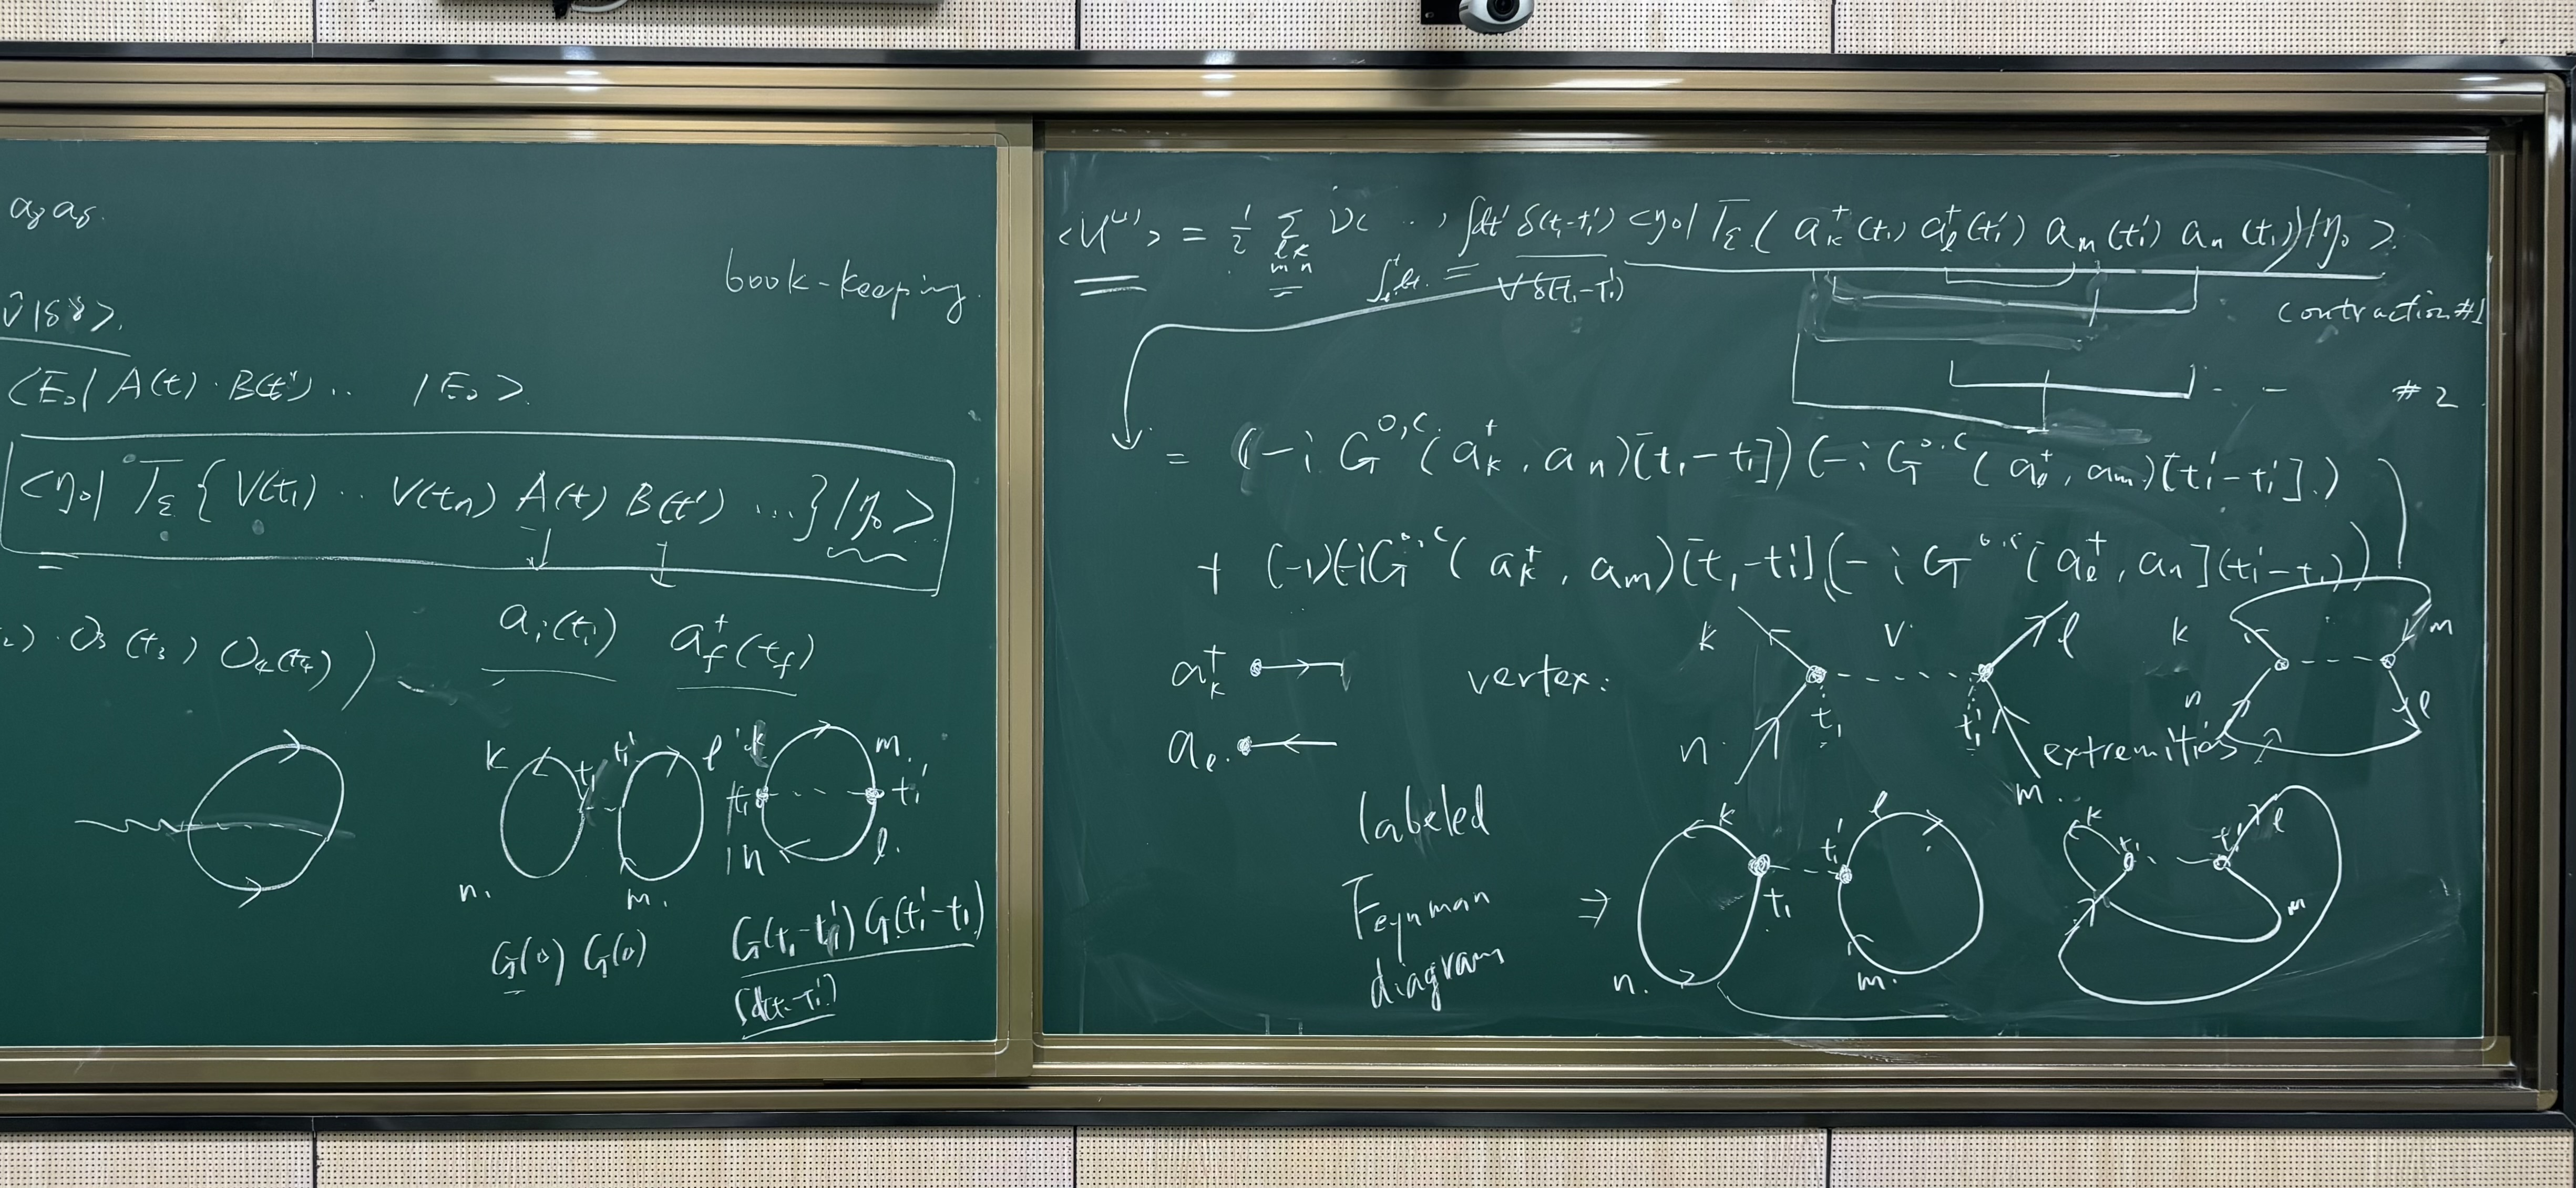
\includegraphics[width = \linewidth]{./media/feynmann1.jpeg}
\end{center}
The operators and the vertices
$
  a_k^\dagger:
  \tikz[baseline]
    { \fill (0,0) circle (.1); \draw [->] (0,0) -- (1,0);} \quad
  a_k:
  \tikz[baseline]
    { \fill (0,0) circle (.1); \draw [<-] (0,0) -- (1,0);}
$
which form through the labeled Feynman diagram.

\section{Feynman rules for labeled Feynman diagrams}

\begin{equation}
  V = \frac12 \int \d t_1' \delta(t - t_1') V_{klmn}
      a_k^\dagger(t_1) a_l^\dagger(t_1') a_n(t_1')a_n(t_1)
\end{equation}
\begin{center}
  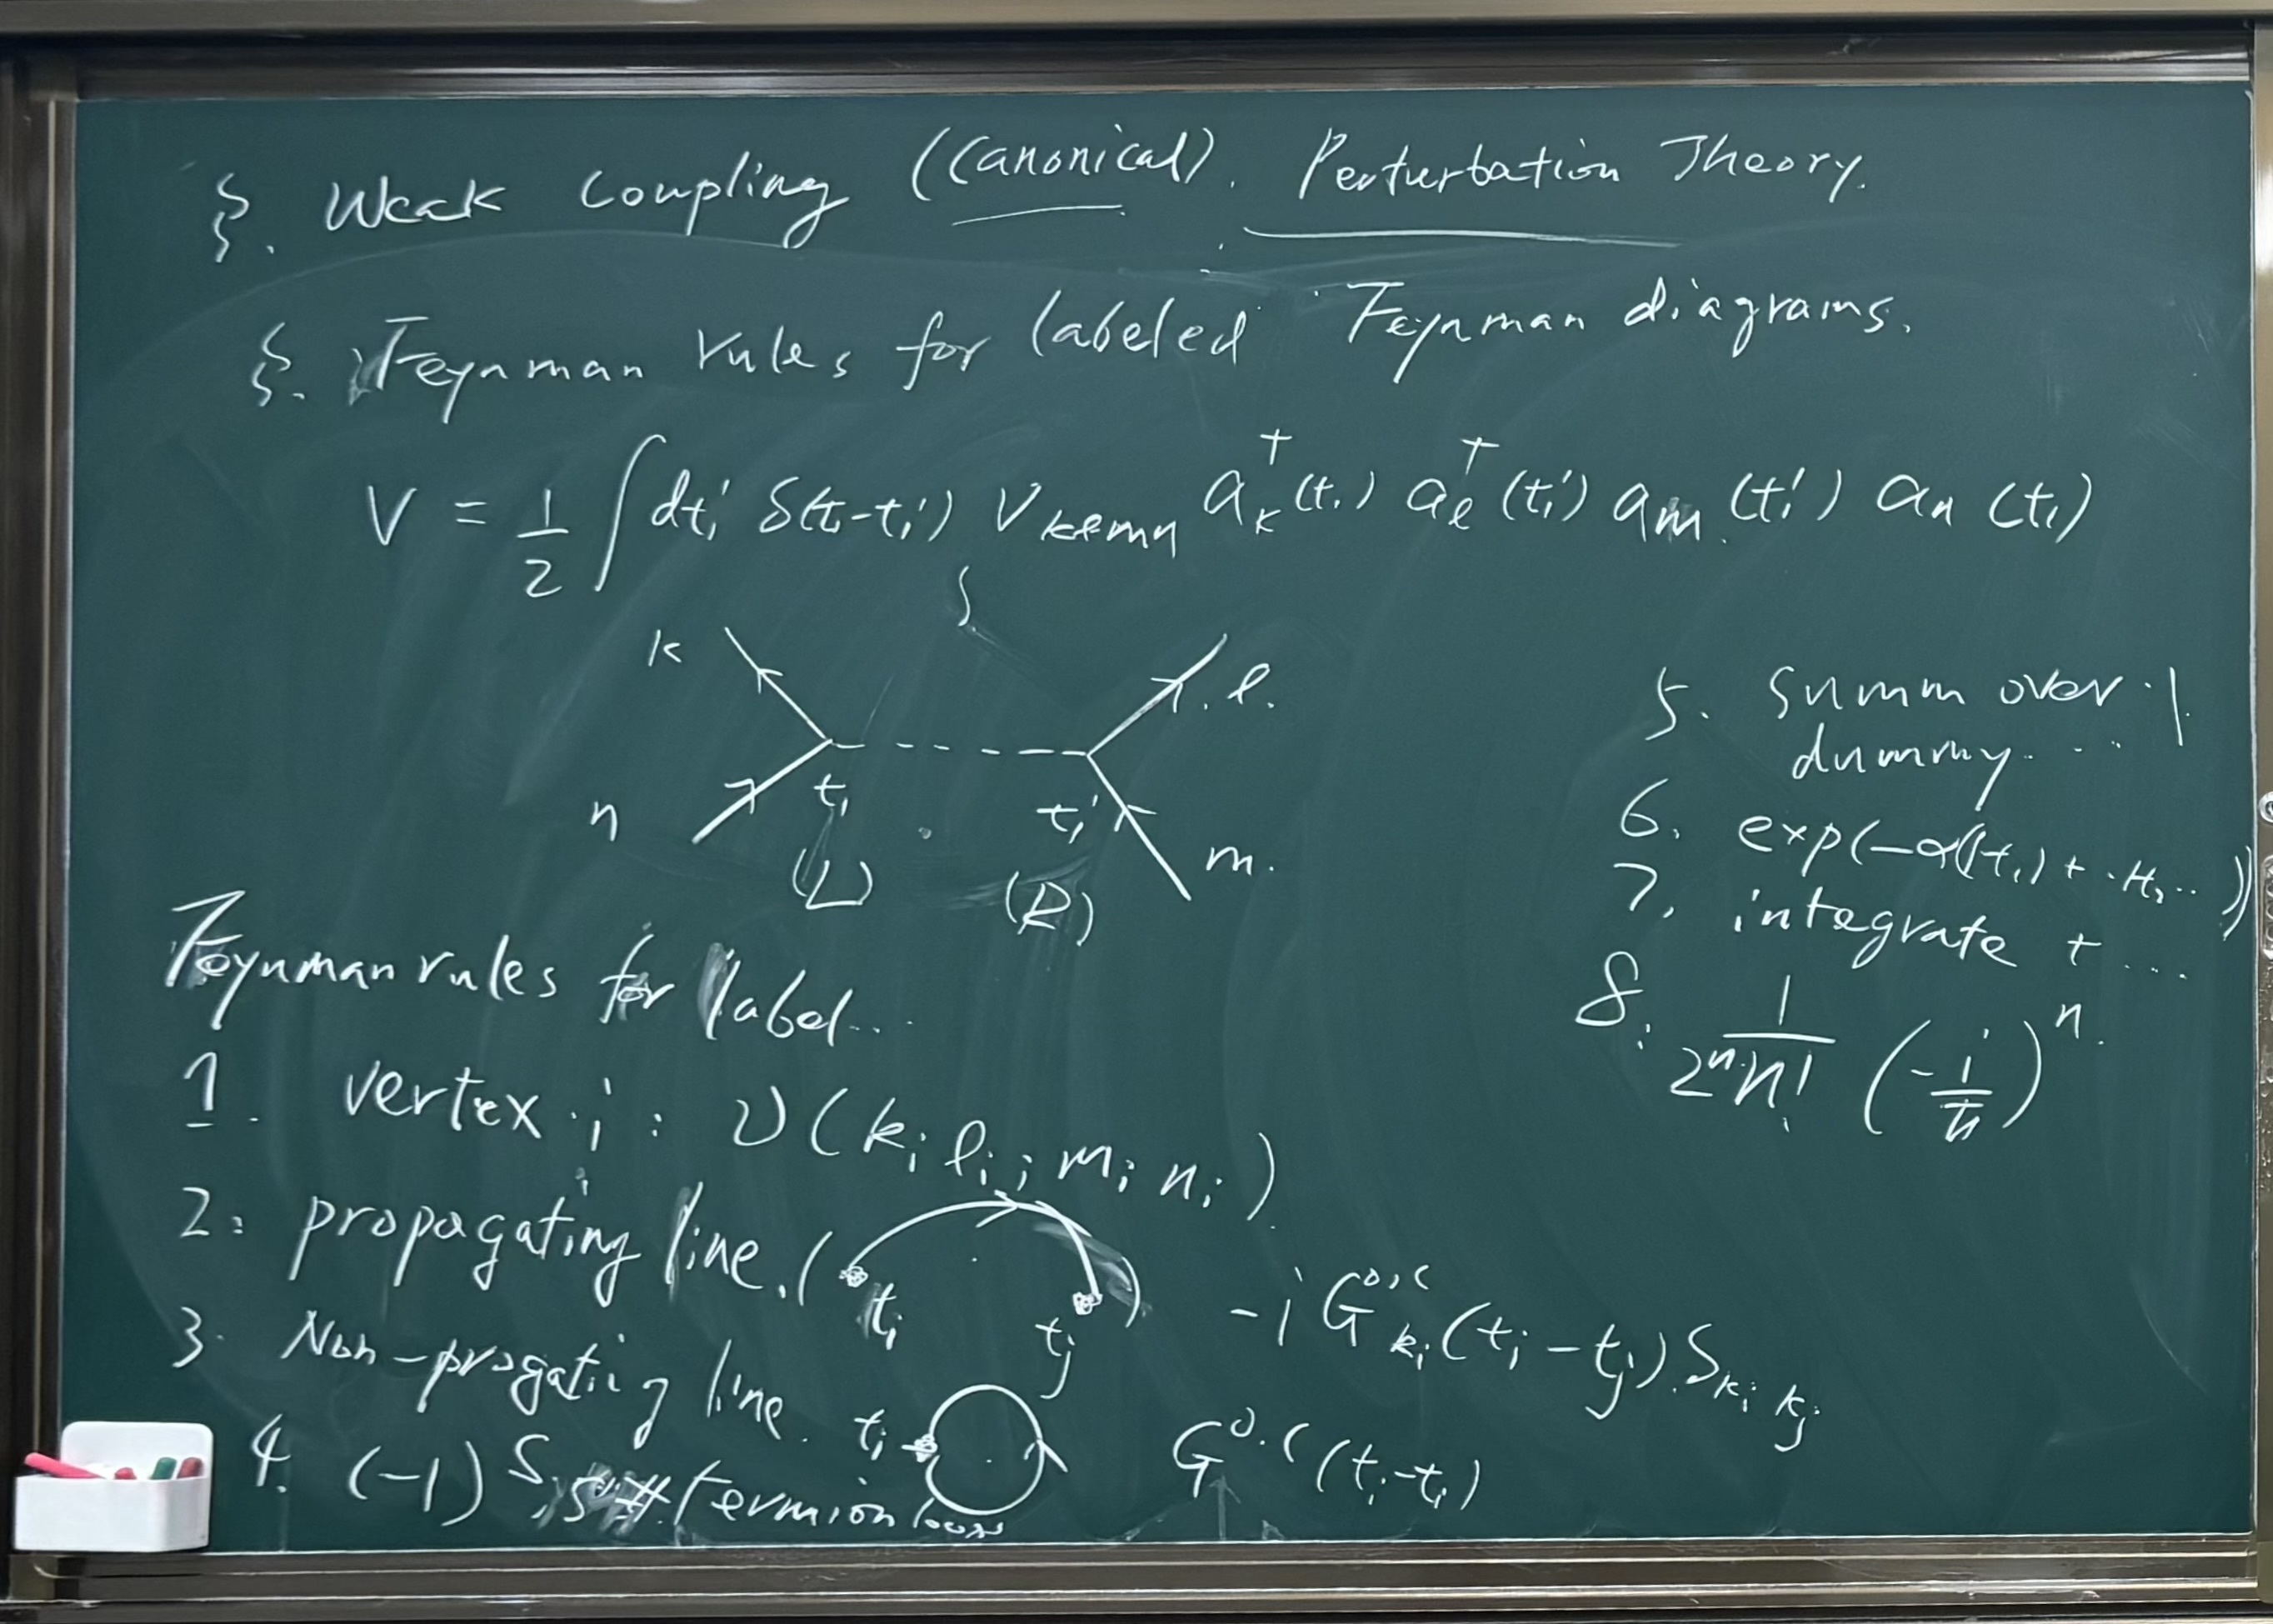
\includegraphics[width = \linewidth]{./media/feynmann2.jpeg}
\end{center}
For $\braket<lk|\hat V|mn>$, if one switch $\braket<k(L)l(R)|\hat V|n(L)m(R)>$,
then the diagram will be flipped: permuting extremities($L \leftrightarrow R$).
\begin{enumext}[columns = 2]
  \item Vertex i: $\nu(k_i l_i; m_in_i)$
  \item Propagating line:
  \[
    \tikz[baseline]{
      \fill (0,0) coordinate (a) circle (.1) node [below] {$t_i$};
      \fill (1,0) coordinate (b) circle (.1) node [below] {$t_j$};
      \draw (a) to [bend left = 20] (b);
    } \quad
    -\iu G_{k_i}^{0,c} (t_i - t_j) \delta_{k_ik_j}
  \]
  \item Non-propagating line:
  \[
    \tikz[baseline]{
      \node [left] at (-.25,0) {$t_i$};
      \fill (-.25,0) circle (.05);
      \draw [->] (-.25,0) arc (-180:0:.25);
      \draw (0,0) circle (.25);
  } \quad
    G^{0,c}(t_j - t_i)
  \]
  \item $(-1)^S$, $s$\# fermion loop.
  \item Summ order dummy \dots
  \item $\exp(-\alpha(|t_1| + |t_2| + \cdots))$
  \item Integrate $t$ \dots
  \item $\frac1{2^nn!} \ab(-\frac\iu\hbar)^n$
\end{enumext}

\section{Unlabeled Feynman diagram \# of labeled diagram $\mathrm{(2\eta)!}$}

\begin{center}
  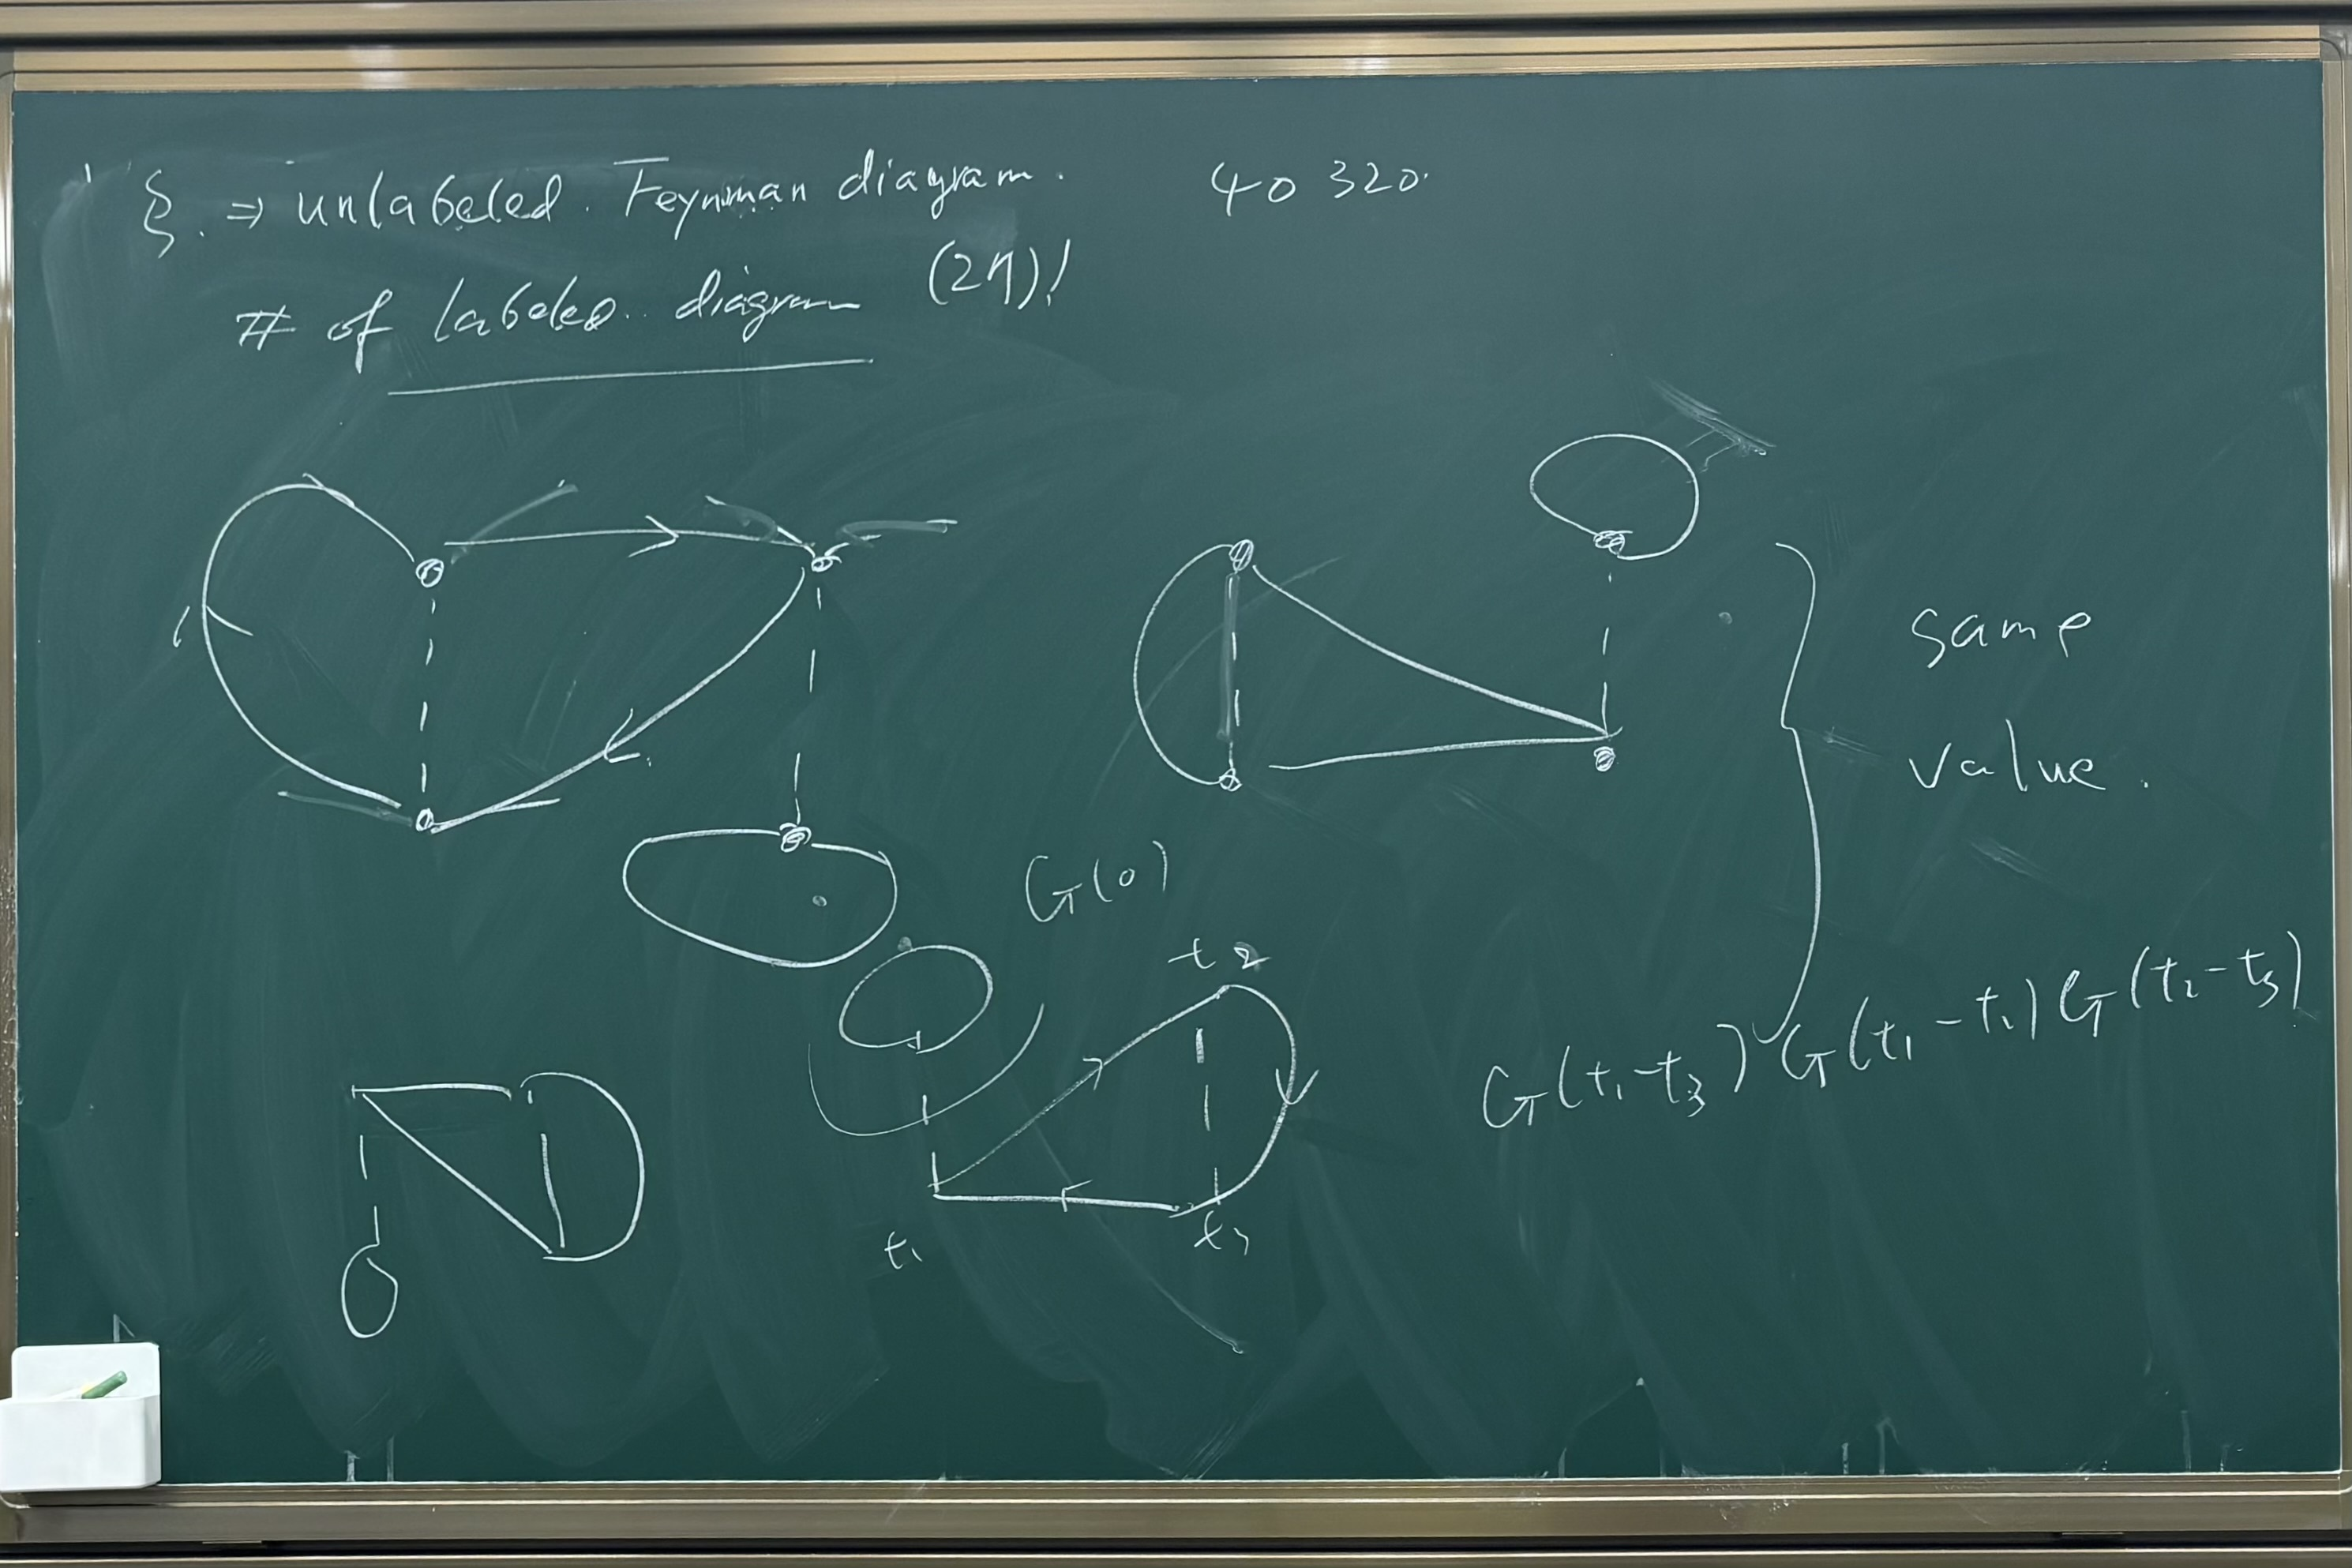
\includegraphics[width = \linewidth]{./media/feynmann3.jpeg}
\end{center}
we can integrate over
\begin{equation}
  G(t_1 - t_3) G(t_1 - t_2) G(t_2 - t_3)
\end{equation}
in these Feynman diagrams.

\section{Remove labels, get right results}

\begin{enumext}
  \item Diagram with same ``topology'' (means classification in math)
  hvae the same value
  \item Given all top. inequ diagram how we count them?
\end{enumext}
\begin{equation}
  \sum_{n_0}\{\text{All contractioin} =\}
\end{equation}
\begin{center}
  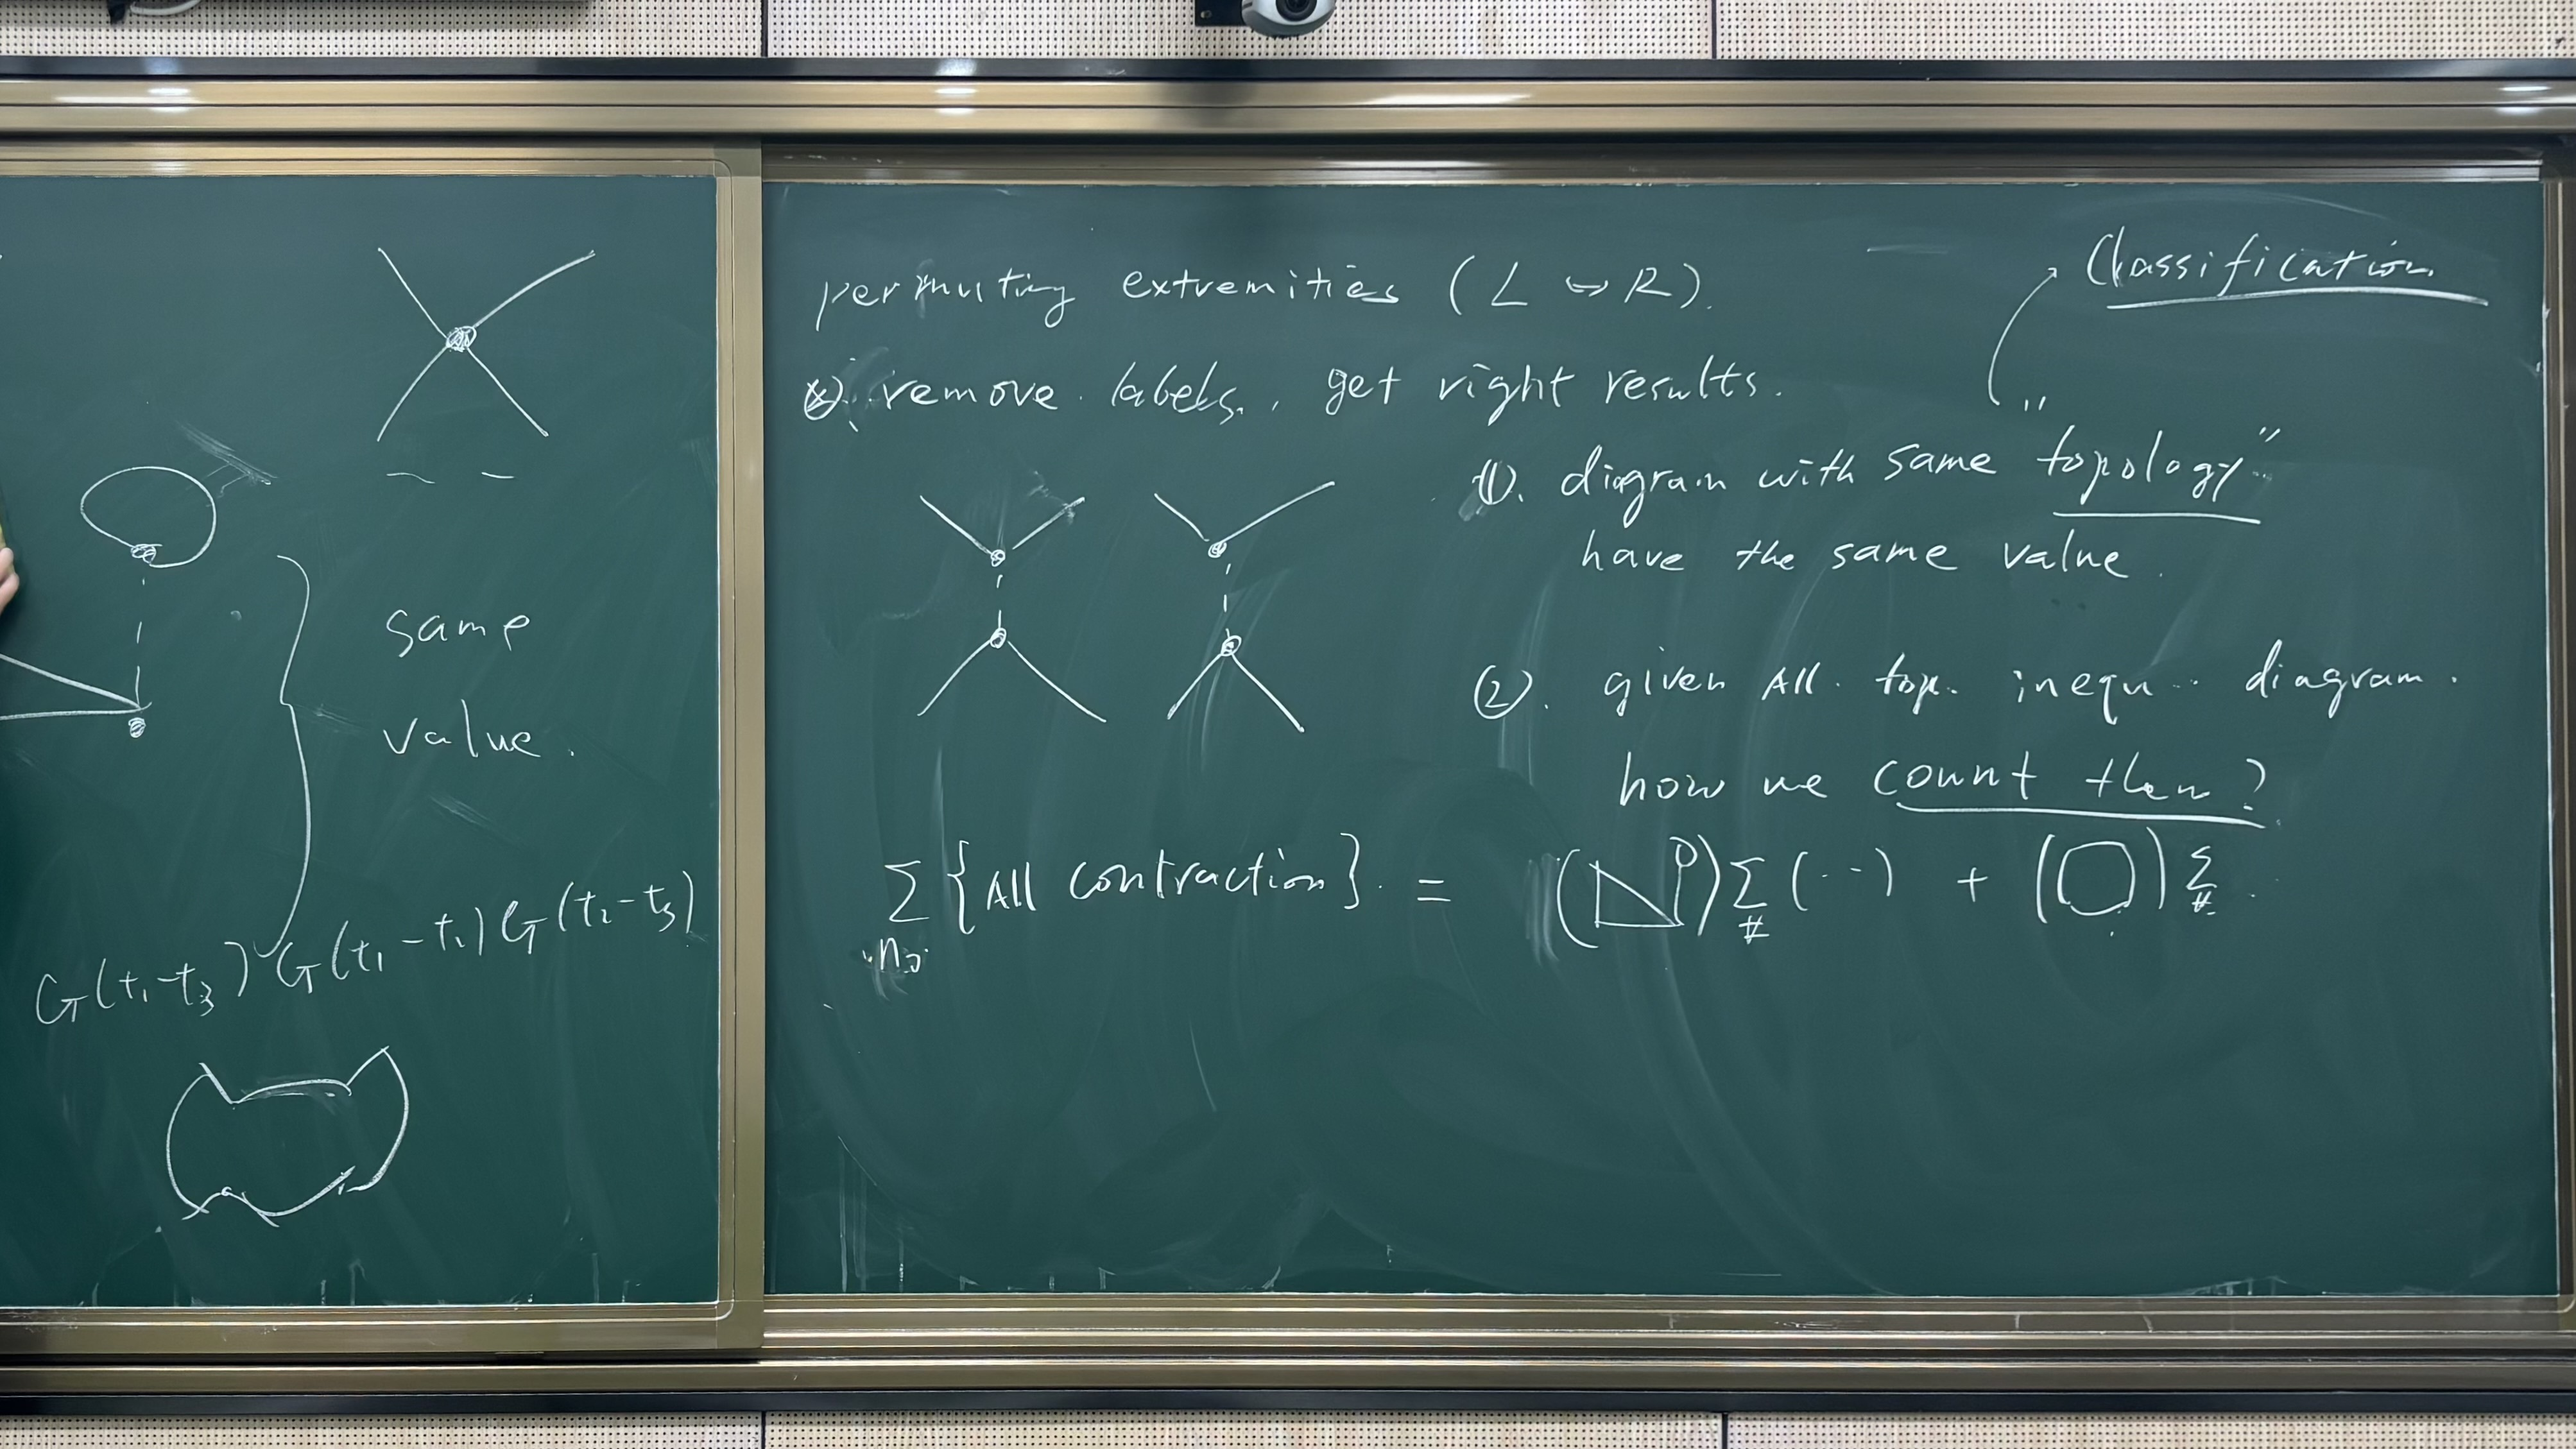
\includegraphics[width = \linewidth]{./media/feynmann4.jpeg}
\end{center}

Transformations of $\Gamma \to \Gamma'$,
but leave  it's value unchanged.
\begin{center}
  Symmetry factor.
\end{center}
We put the labes backing: $k$, $l$, $n$, $m$.

\paragraph{Transformation}
Leaves two structures
\begin{enumext}[columns = 2]
  \item Value unchanged
  \item Diff contraction.
\end{enumext}
Two type of transformations ([Ref] Coloman: symmetry factor):
\begin{enumext}[columns = 2]
  \item Permute extremities.
  \item Propagating lines.
\end{enumext}
\begin{center}
  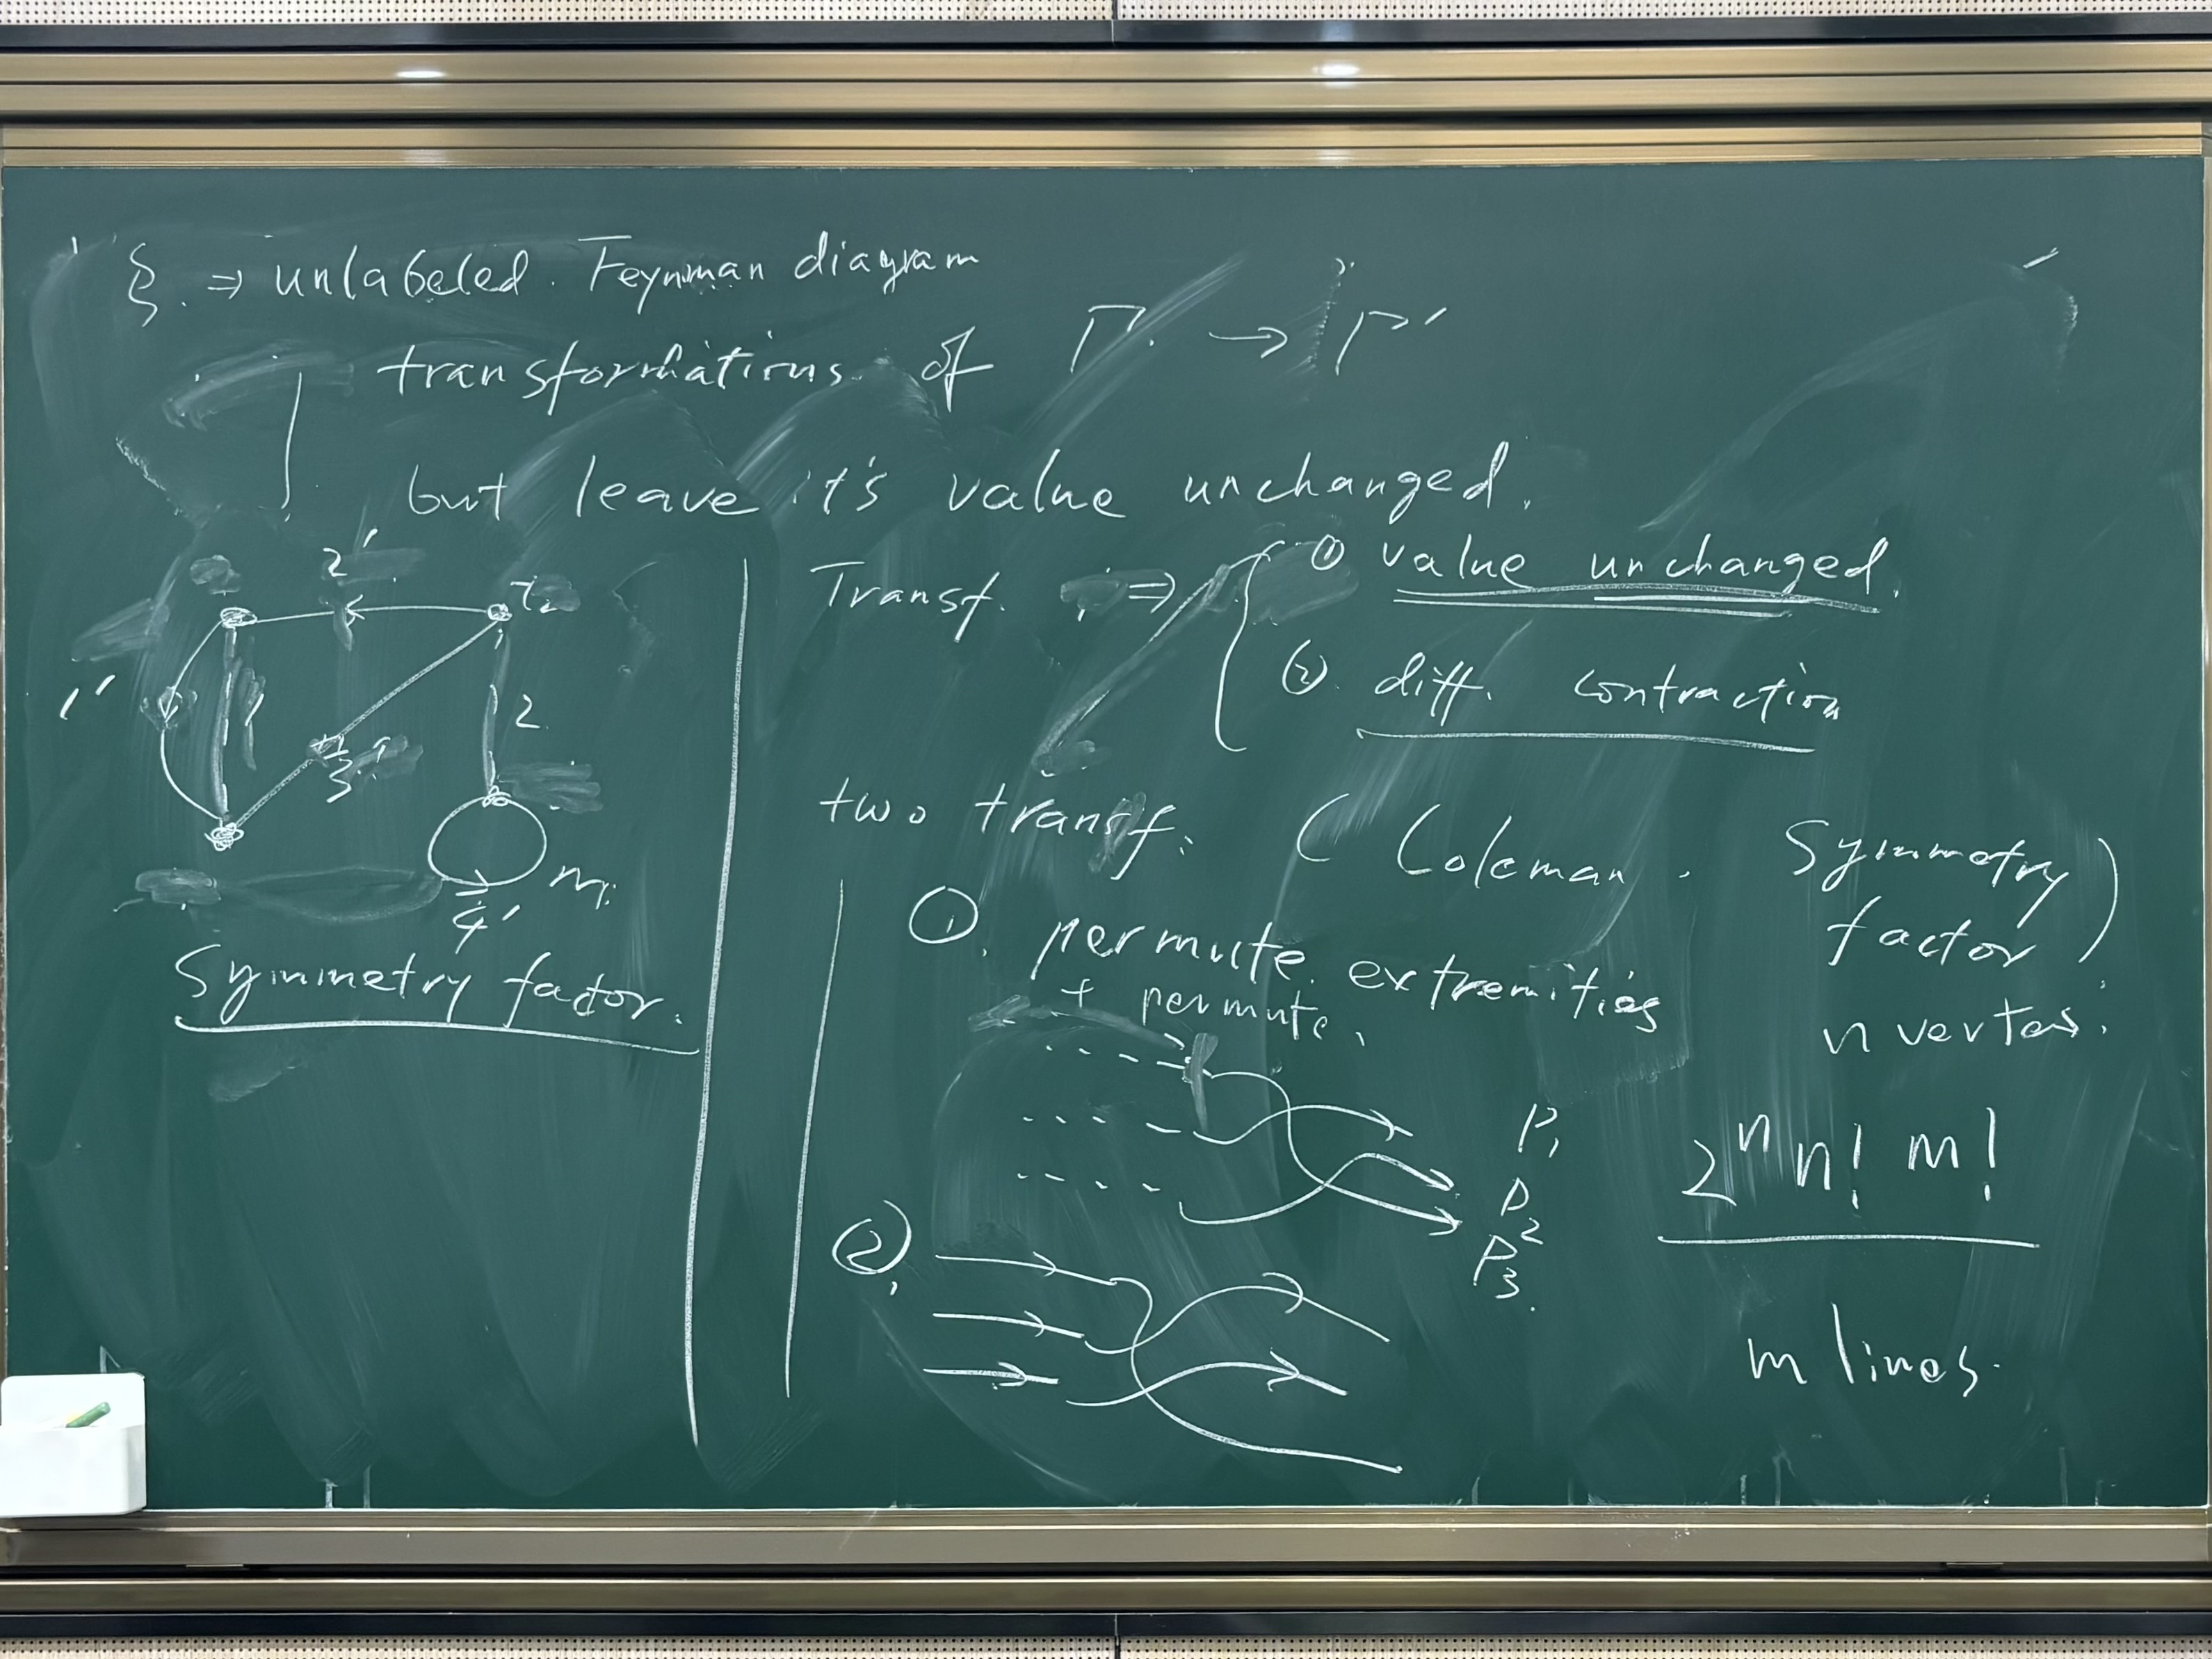
\includegraphics[width = \linewidth]{./media/feynmann5.jpeg}
\end{center}
If we have $n$ vertices and $m$ lines, and this will give
$2^nn!m!$ possibilities.

All these transf leave value unchange, but
\begin{enumext}[columns = 2]
  \item Different contraction (labeled diag)
  \item Same contraction \texttt{->} over counting
\end{enumext}
The sum
\[
  \sum\{\text{All contractions}\}
\]
Symmetry factor: account for overcounting.
The flips come from the transformations
\begin{center}
  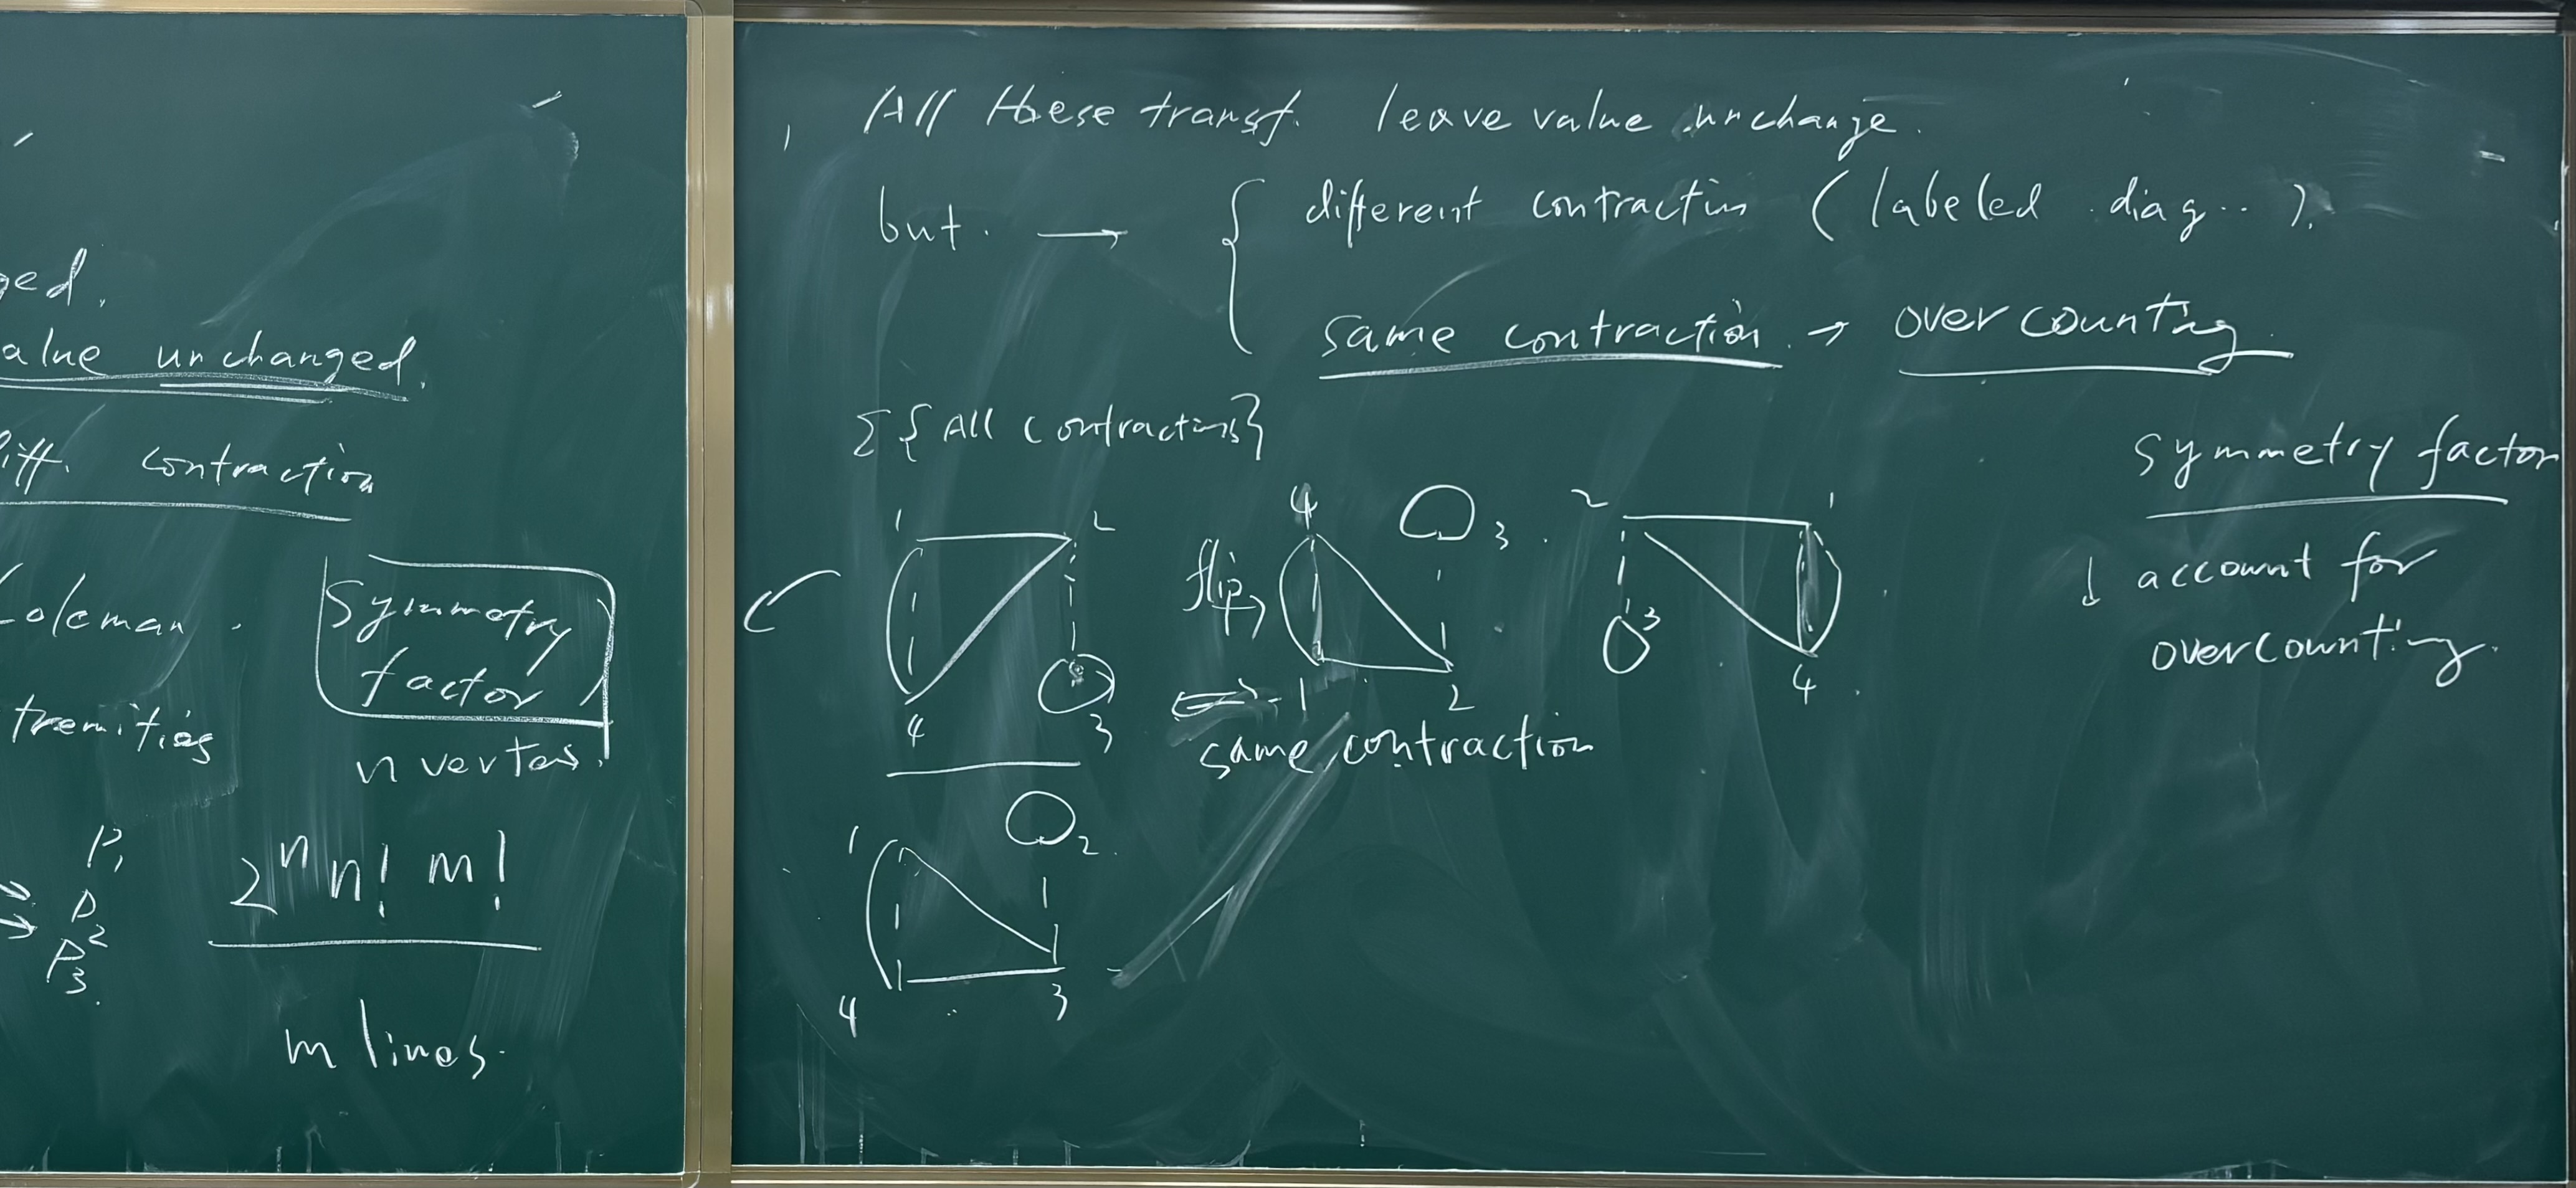
\includegraphics[width = \linewidth]{./media/feynmann6.jpeg}
\end{center}

\paragraph{\# Final step}
Obtain the symmetry factor $S$.
\begin{enumext}
  \item All pass: value-inv.transf $G$.
  \item $G_\Gamma$: Transf $\Gamma$ into a deformations (same contraction)
  of itself. Hence, $G_\Gamma$ is sub group of $G$.
  \item $S = \#$ of elements of $G_r$, $S$ must be divisor of $2^nn!m!$.
\end{enumext}

\section{Unlabeled Feyman diagram}

Using label permutation to obtain $S$, $\Gamma'$
\[
  G_\Gamma: \mathcal G\{(12), (21)\}
\]
means $1 \to 2$ and $2 \to 1$.
\begin{center}
  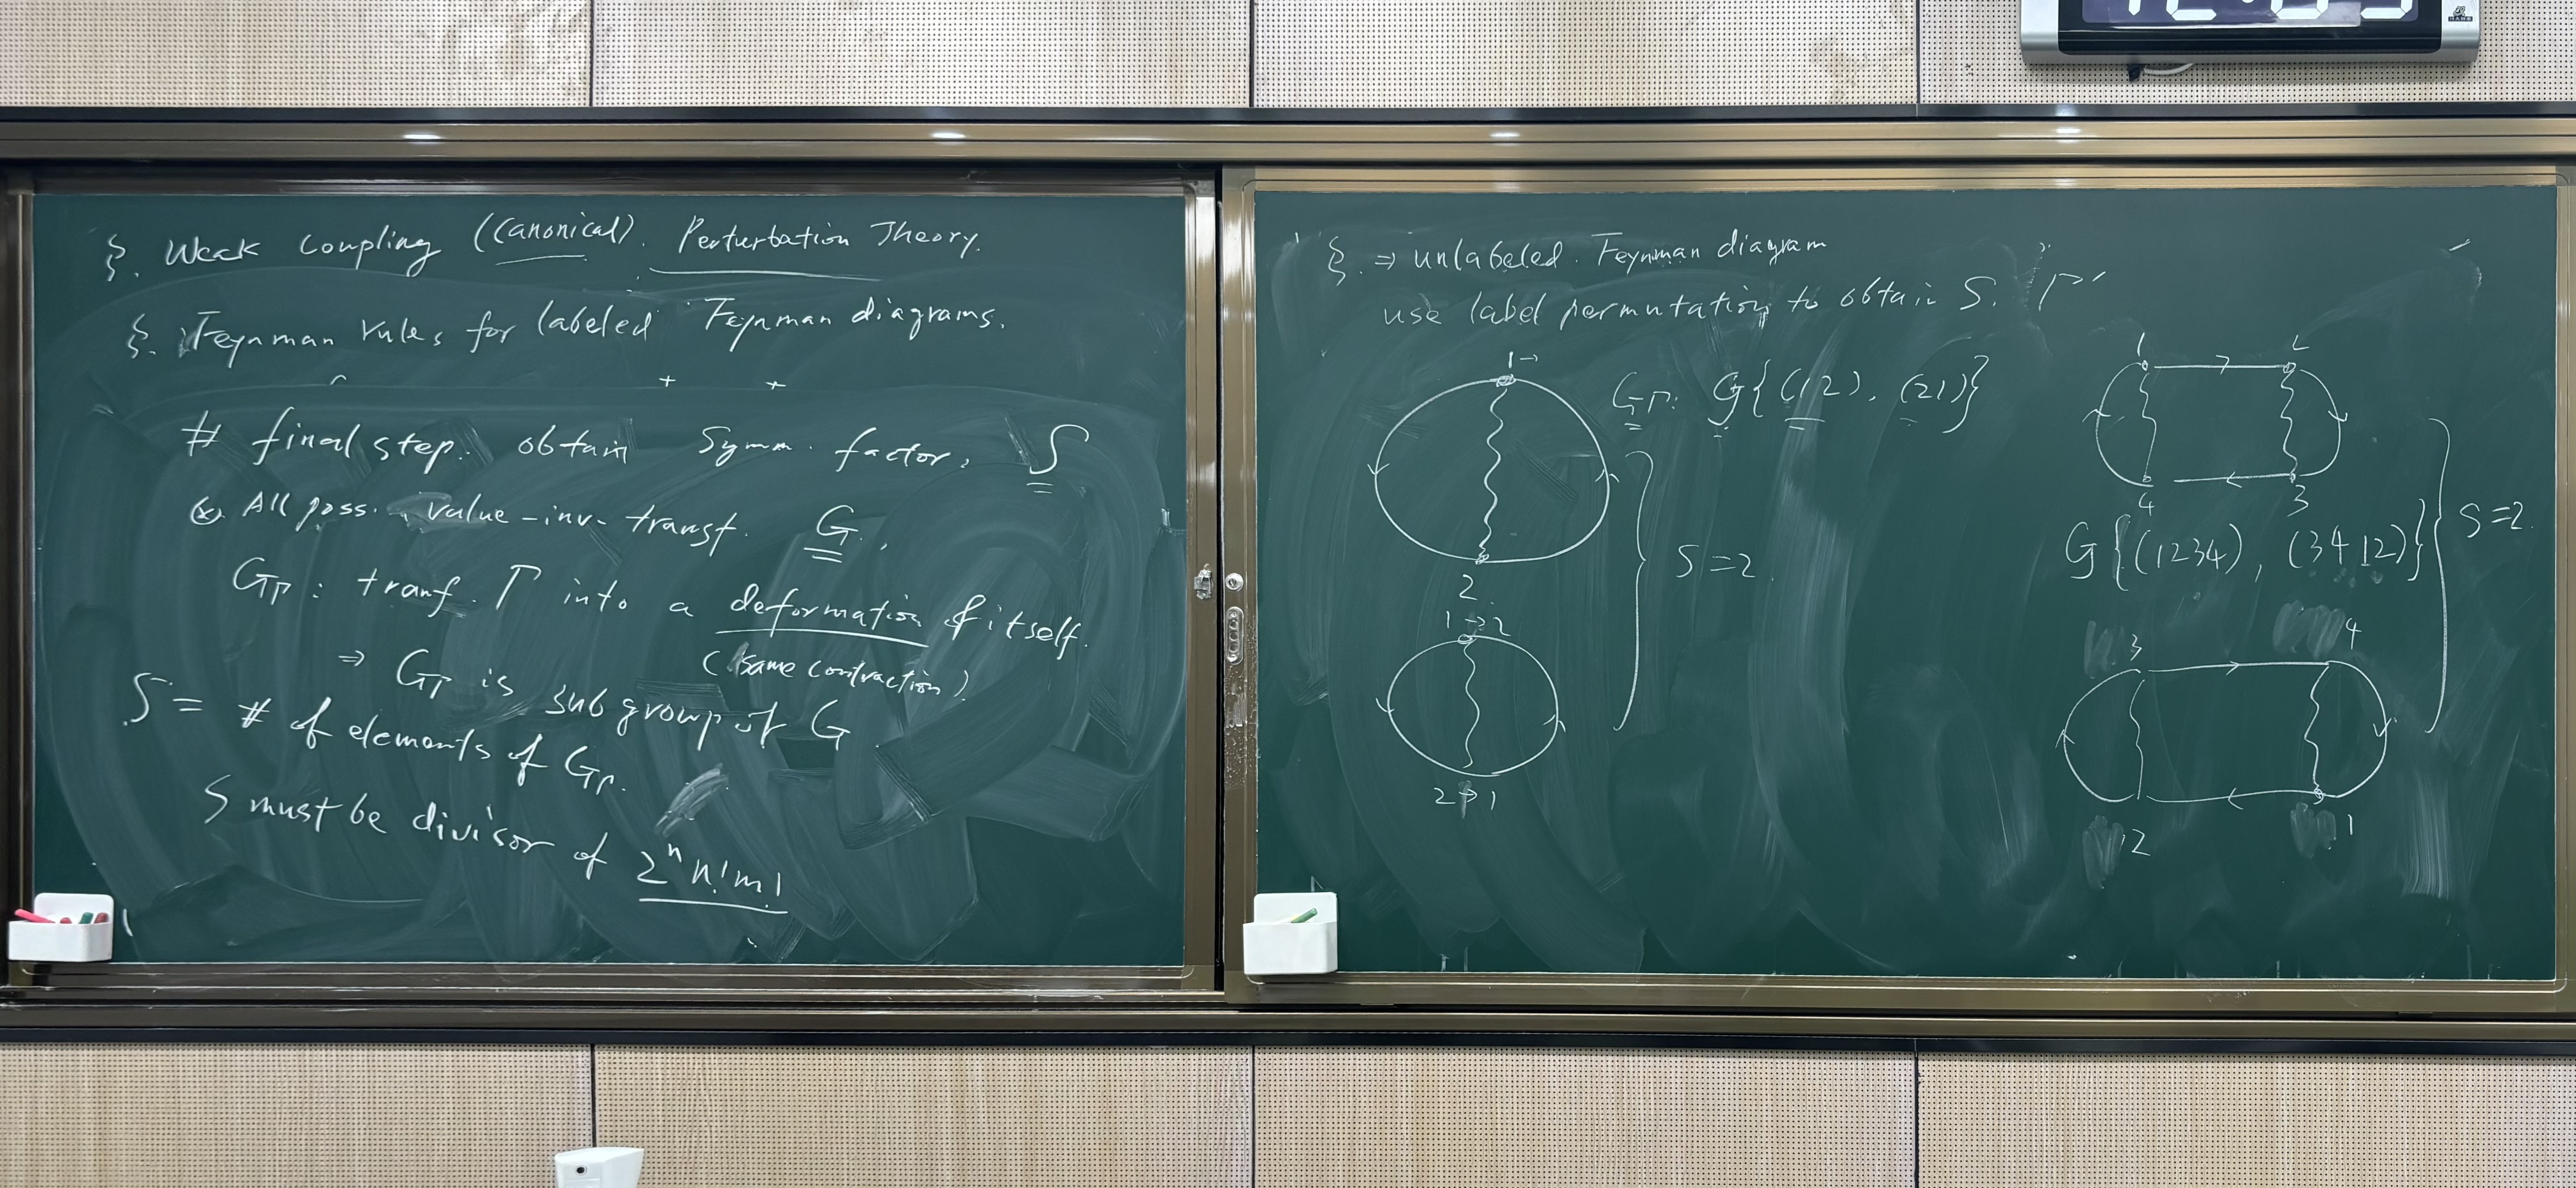
\includegraphics[width = \linewidth]{./media/feynmann7.jpeg}
\end{center}
These diagrams have $S = 2$.
\begin{example}
  Two vertices diagram $\mathcal G\{(1234), (3412)\}$. Using label Pertubation:
  $1 \to 3$, $2 \to 4$, $3 \to 1$, $4 \to 2$.
\end{example}
\begin{example}[$(43\ 12) \notin \mathcal G$]
  Diff contraction
\end{example}
\begin{center}
  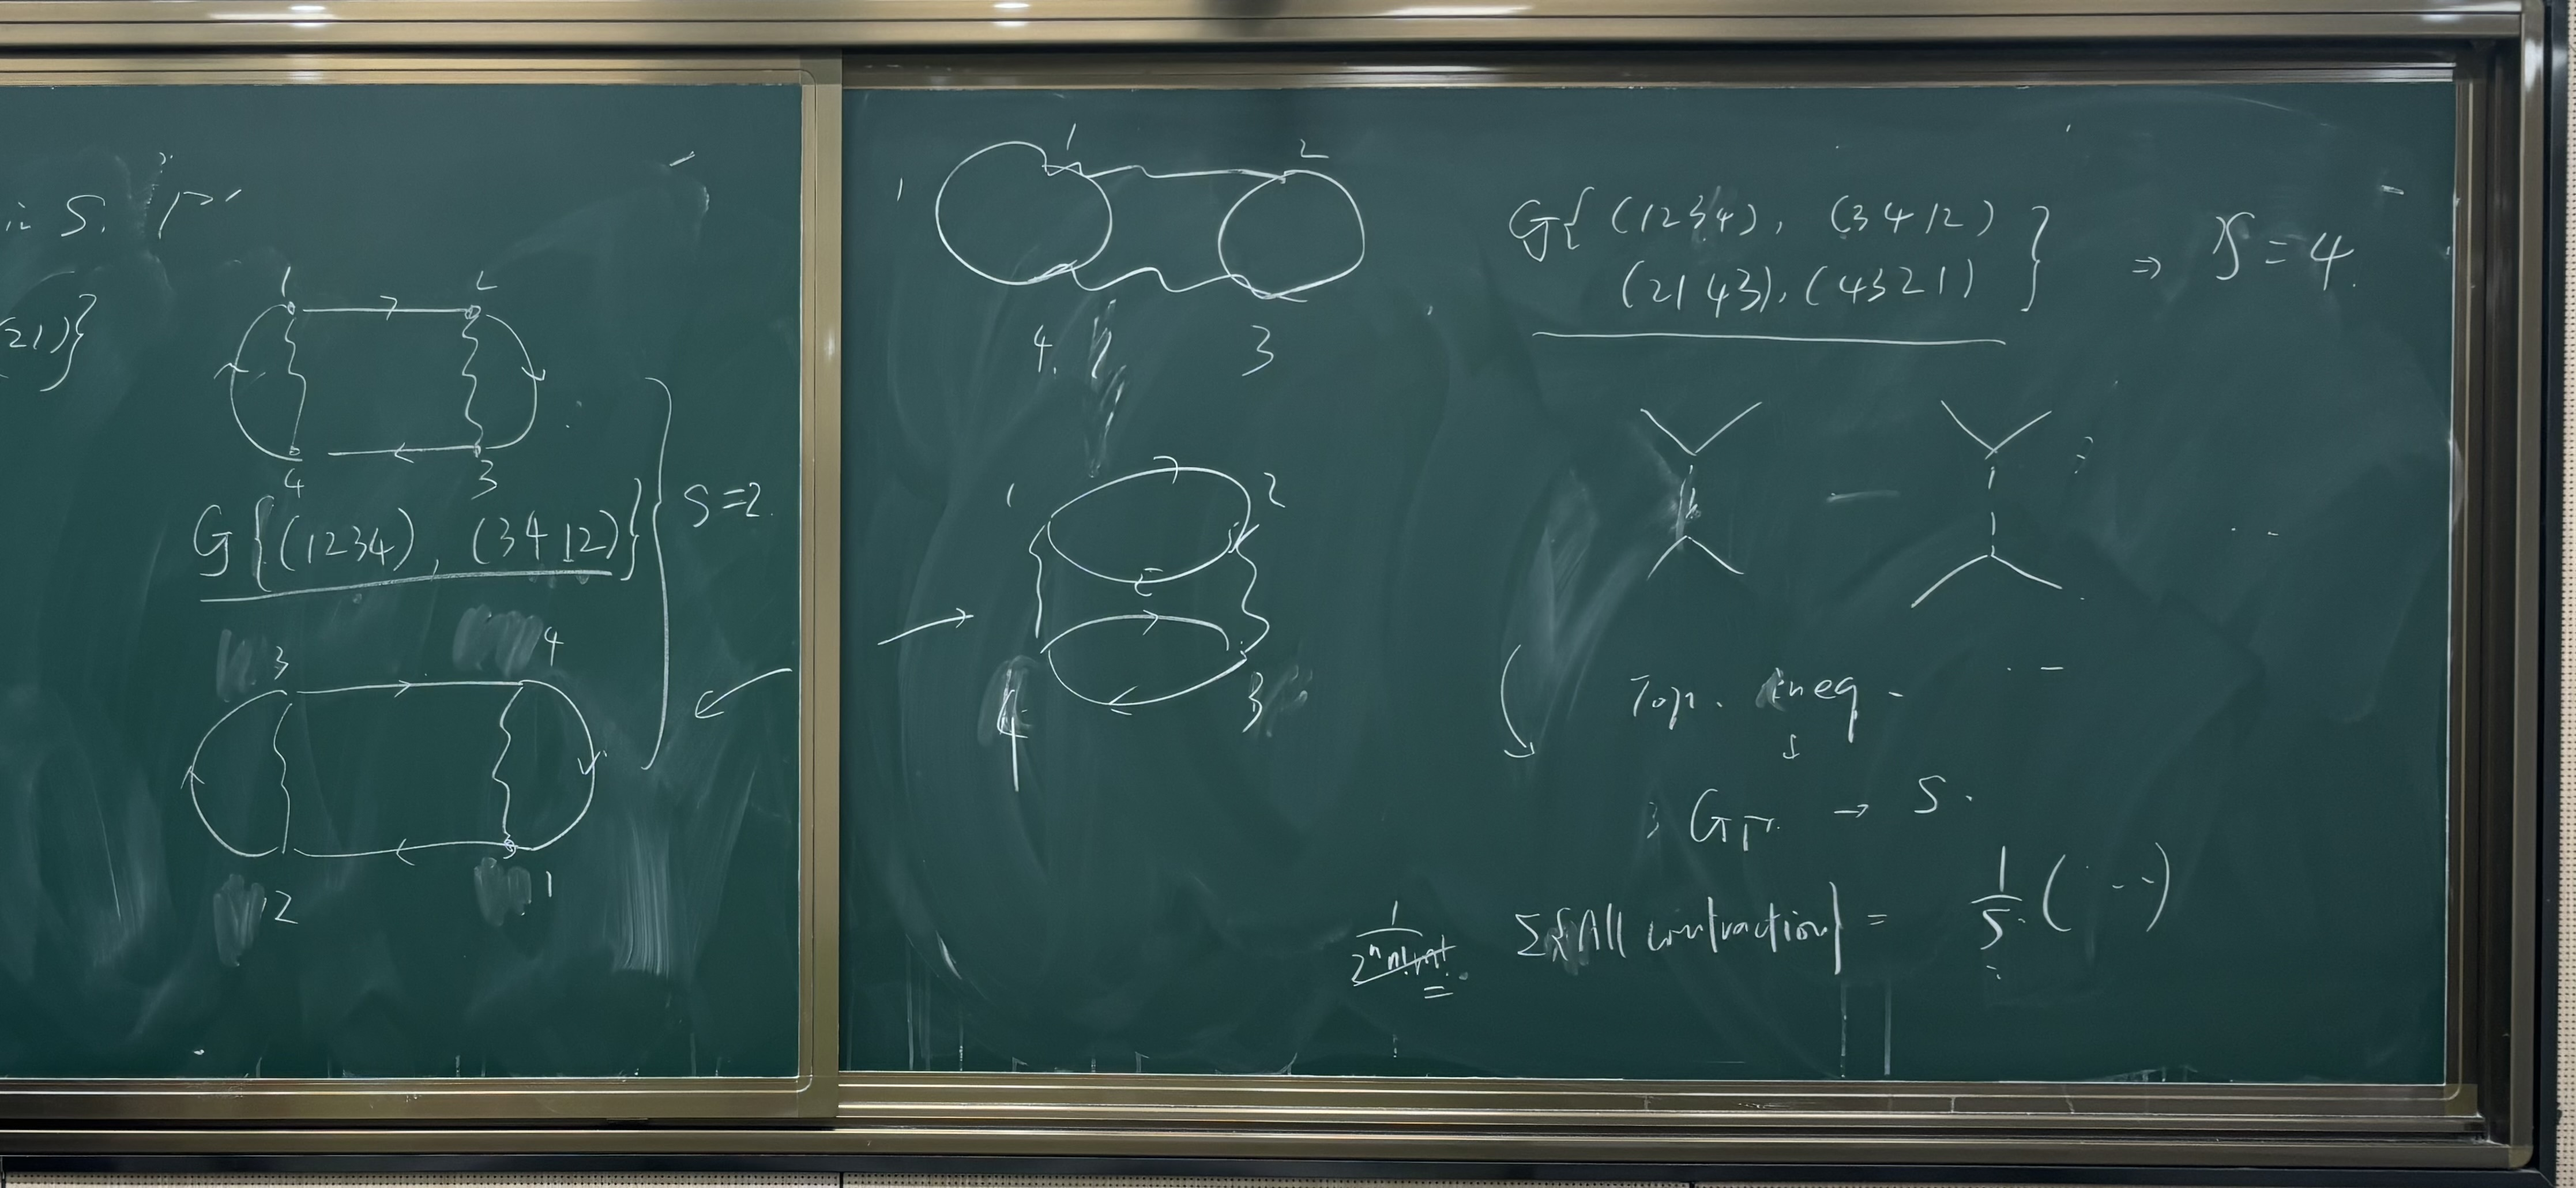
\includegraphics[width = \linewidth]{./media/feynmann8.jpeg}
\end{center}
\begin{example}
  Compare with two diagrams
  \[
    \mathcal G\{(1234), (3412), (2143), (4321)\} \to S = 4
  \]
  Combines them Topo ineq.
  \[
    G_\Gamma \to S, \quad
    \cancel{\frac1{2^nn!m!}} \sum\{n\|\text{contraction}\} = \frac1s (\cdots)
  \]
  which cancels by ``All poss value-inv-transf'', for $v = \frac12$.
\end{example}

\section{Labeled Feynman Diagram}

\[
  \begin{tikzpicture}[baseline]
    \draw [->] (-1,-1) node [left] {$c_\beta$} -- (0,0) -- (-1,1)
     node [left] {$c_\alpha^\dagger$};
    \draw [dashed] (0,0) -- (1,0);
    \draw [->] (2,-1) node [right] {$c_\sigma$} -- (1,0) -- (2,1)
     node [right] {$c_\gamma^\dagger$};
  \end{tikzpicture}
  \longrightarrow
  \sum\text{Contraction} =
  \sum_{\substack{\alpha\beta\\\gamma\sigma}}
\]
Permutation of all $b$ vectors,
also to permute all the $m$-propagators: A factor of $2^nn!m!$.
Satisfy the Symmetry
\[
  \wick{\braket<\c\alpha\c\beta|V|\c\gamma\c\sigma>
= \braket<\beta\alpha|V|\sigma\gamma>} \to 2^nn!m!
\]
\begin{center}
  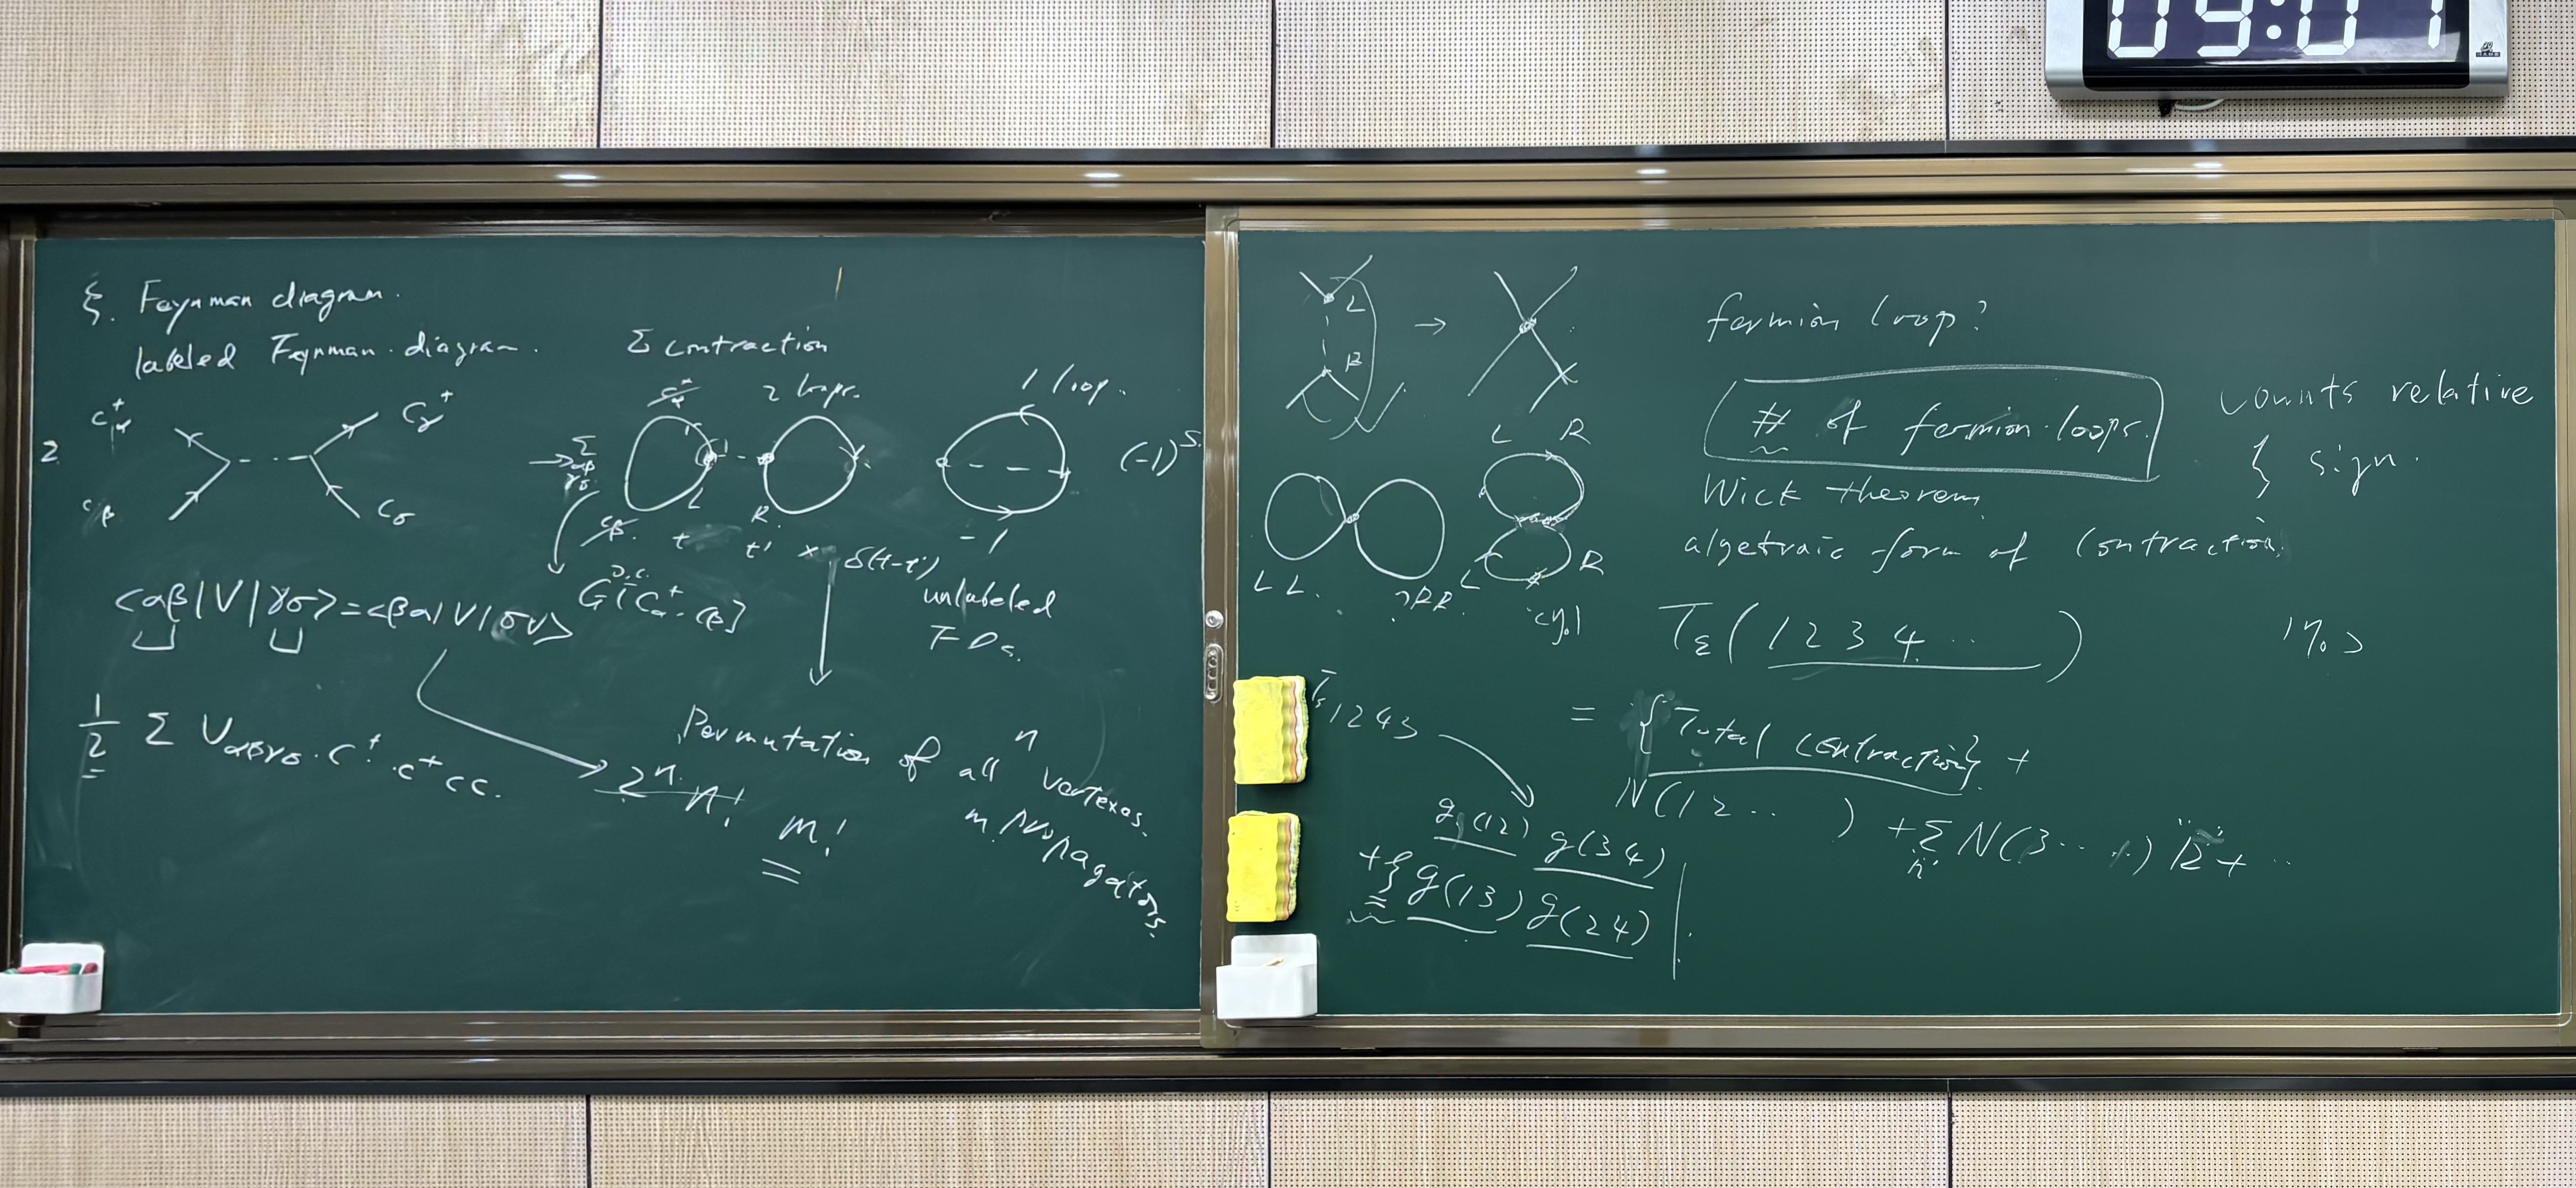
\includegraphics[width = \linewidth]{./media/feynmann9.jpeg}
\end{center}

\subsection{Wick theoremm: algebraic form of contraction}

\[
  \braket<\eta_0|T_\epsilon(1234 \cdots)|\eta_0>
= \{\text{Total contraction}\} + N(12\cdots) + \sum_{``12''} N(3\cdots) ``12'' + \cdots
\]
For $4$ operators: $T_\epsilon \to g(12)g(34) + \xi g(13)g(24)$, give a counts relative $\eta$ sign.
\subsection{Permutation counting}

\[
  2^nn!m! \to \text{perm identical progators}
\]
In QFT bosonic $\phi^4$-theory, it gives a huge counting $m!$ of propagator.
\[
  \to \frac1S, \qq{$S$ is symmetry factor.}
\]
\begin{center}
  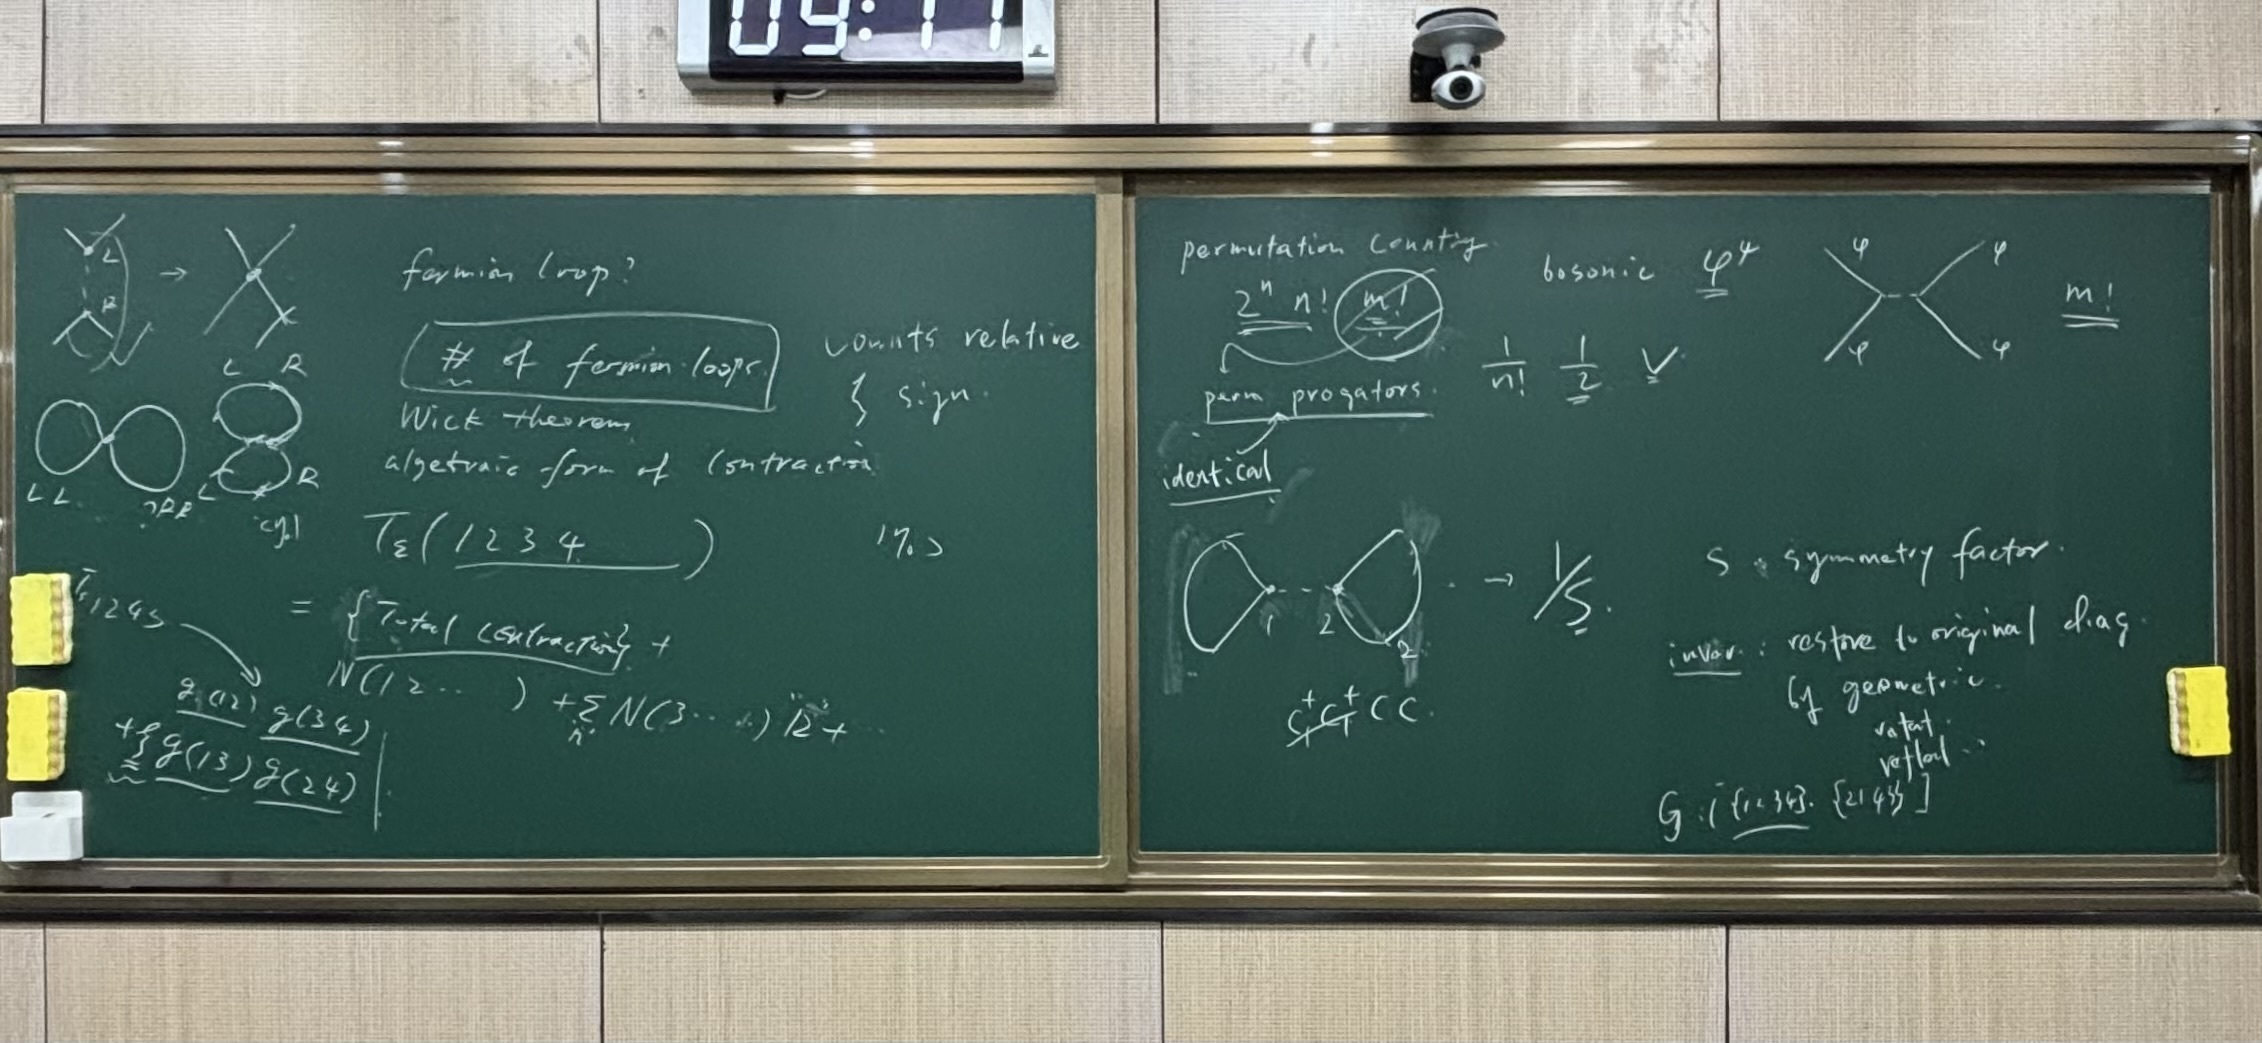
\includegraphics[width = \linewidth]{./media/feynmann10.jpeg}
\end{center}
Invariant: restore to original diagram by geometric ratat reflact
$\mathcal G:\ [\{1234\}, \{2143\}]$

\subsection{Linked cluster theorem}

\begin{equation}
  \braket<\eta_0|U_\alpha(t,t')|\eta_0>
= \exp\ab\{\sum_\nu^\text{connected} U(\Theta_v)\}
\end{equation}
where $v$ denotes the order of diagrams (\# of vertexes),
$\Theta$ gives the structure (Topology) of the diagram.
``Connected'' means the contractions which cannot be separated without cutting
any line.
\begin{center}
  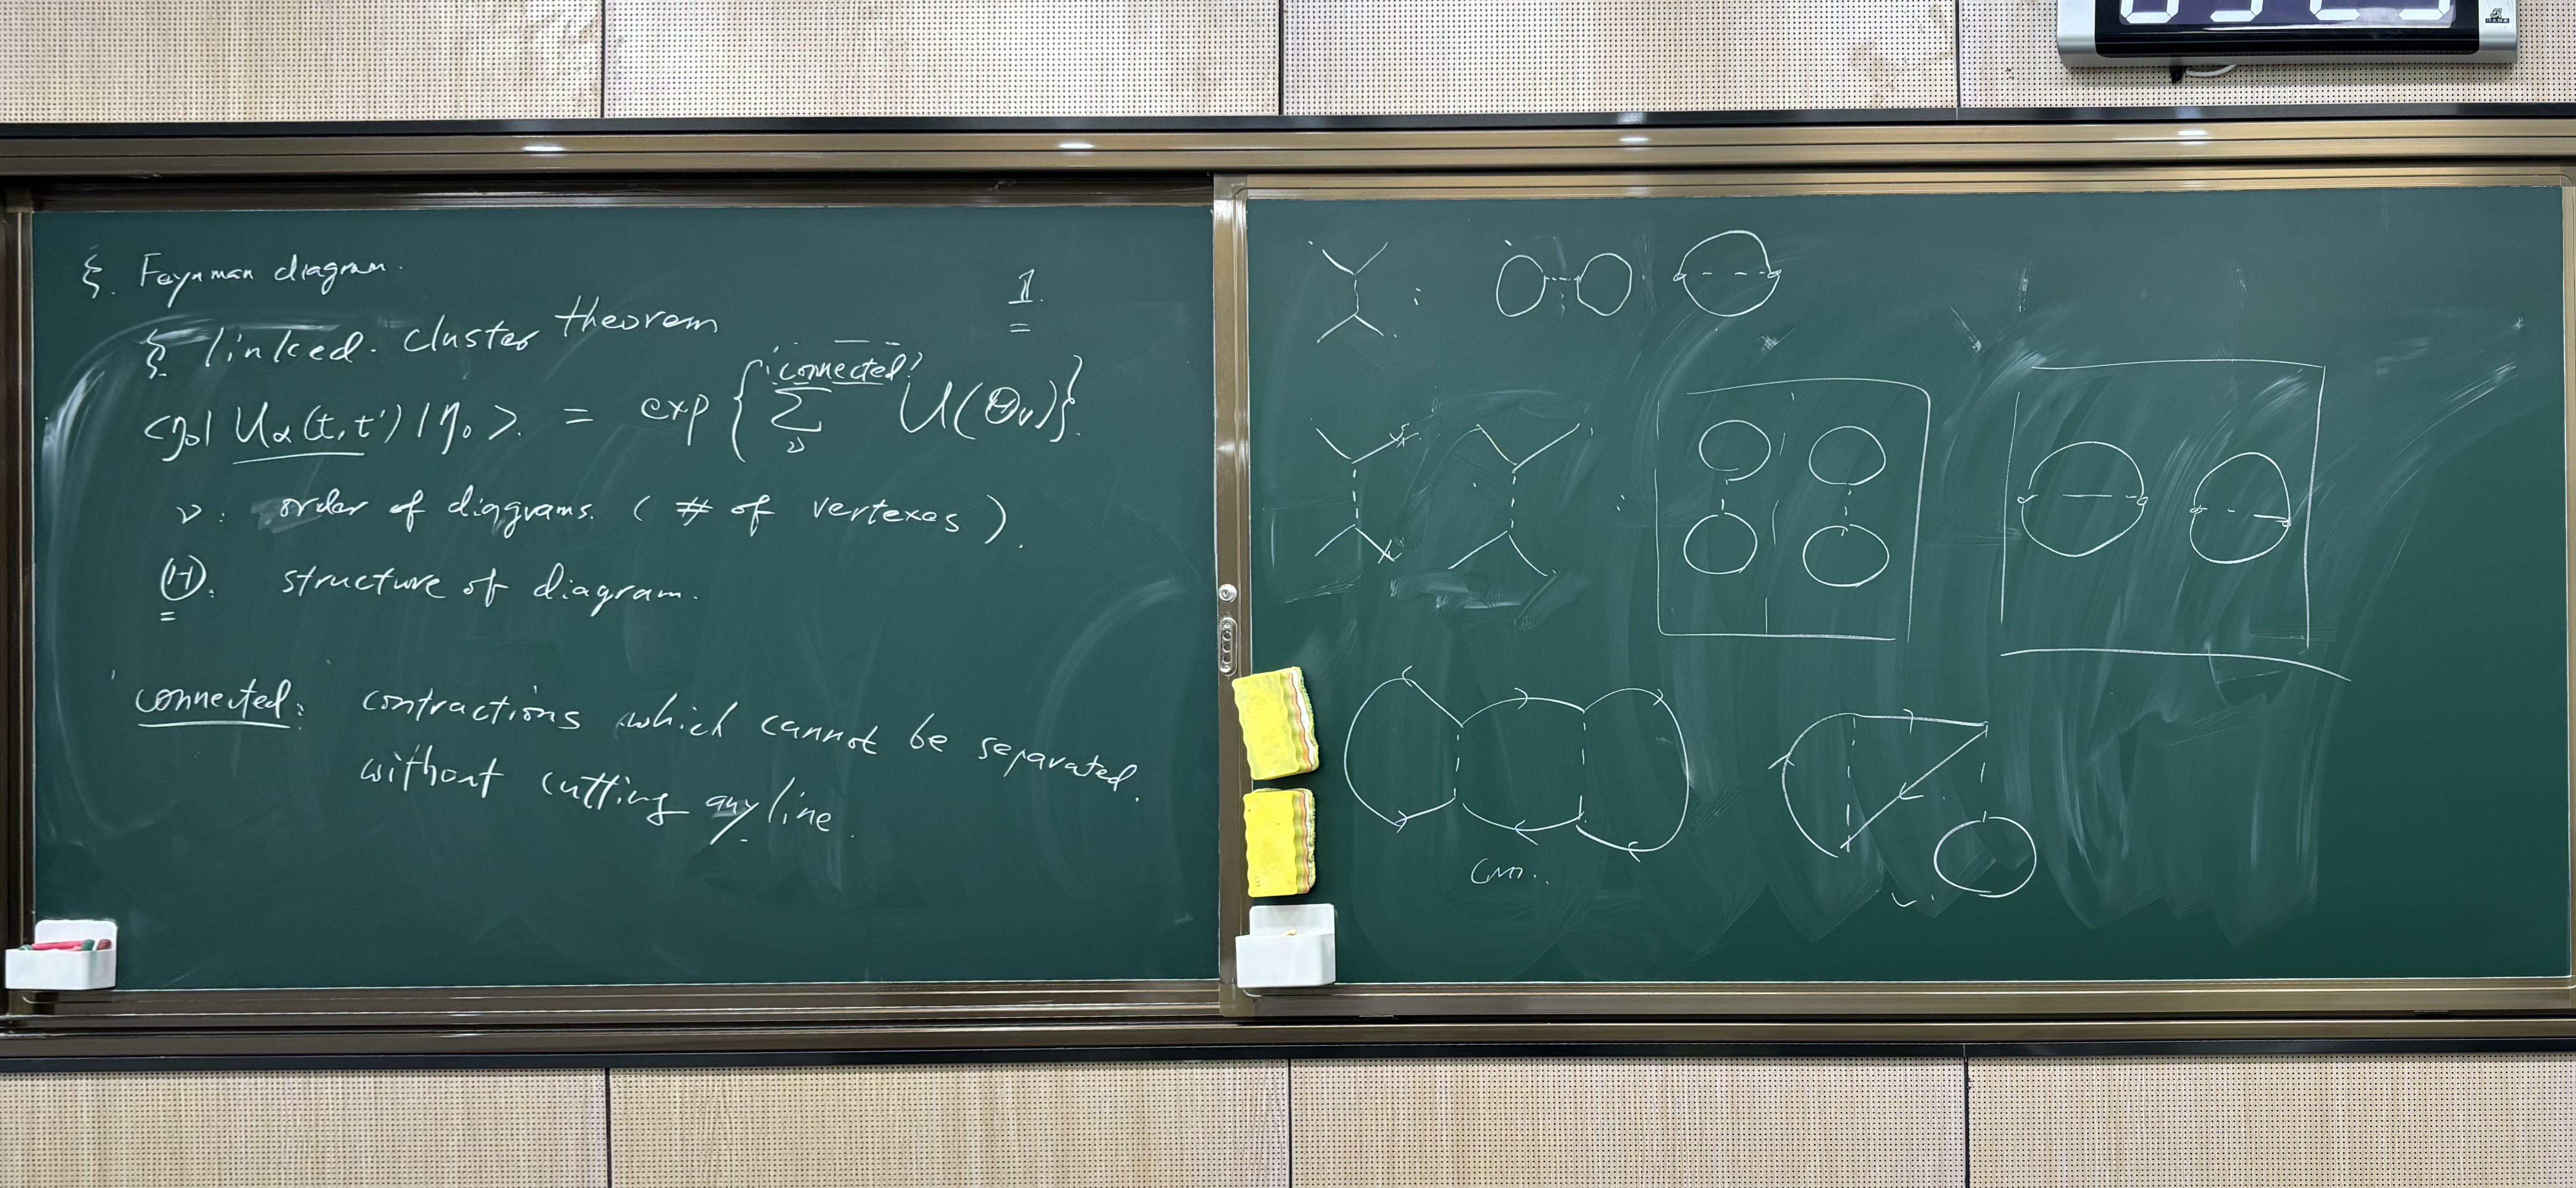
\includegraphics[width = \linewidth]{./media/feynmann11.jpeg}
\end{center}
\begin{enumext}[columns = 3]
  \item All contractions
  \item All connected
  \item All paths
\end{enumext}
So, the expression can be expanded
\[
  \braket<\eta_0|U|\eta_0>
= \sum_\nu \frac1{\nu!} \braket<\eta_0|T_\epsilon\{V_1V_2\cdots V_\nu\}|\eta_0>
\]
All contractioins reducible
\[
  U(\Theta_\nu) = U^*(\Theta_{\nu_1}) U^*(\Theta_{\nu_2}) \cdots
                  U^*(\Theta_{\nu_k})
\]
If inreducible / connected
\[
  U(\Theta_\nu) = U^*(\Theta_{\nu})
\]
\begin{example}
  \[
    U(\Theta) = U(\Theta_1)U(\Theta_2),\ \Theta_1 \neq \Theta_2
  \]
  If $\Theta_1 = \Theta_2$, $U(\Theta) = \frac1{2!} U(\Theta_1)U(\Theta_2)$.
  An arbitrary diagram
  \[
    \Theta = p_1\Theta_1 + p_2\Theta_2 + \cdots + 2 \times p_n\Theta_n
  \]
  where $\Theta = 2\times ``8'' + ``O''$.
  \[
    U(\Theta) = \frac1{p_1!}(U(\Theta_1))^{p_1} \cdots
                \frac1{p_n!}(U(\Theta_n))^{p_n}
  \]
  and the expactation
  \begin{align*}
    \braket<\eta_0|\cdots|\eta_0> = 1 + \sum_\Theta U(\Theta)
& = 1 + \sum_{\Theta_1\Theta_2} U(\Theta_1) + U(\Theta_2) - U(\Theta_3)
    \to \substack{\frac1{3!}U^{*^3}(\Theta_1)\\
    \frac1{1!}\frac1{2!}U^*(\Theta_1)U^*(\Theta_2)\\U^*(\Theta_3)}\\
& = 1 + \sum_1 U^*(\Theta_1)
  + \sum_{1,1'} \frac1{2!} (U^*(\Theta_1), \cancel{U^*(\Theta_{1'})})
    + \sum_2 U^*(\Theta_2) + \cdots\\
& = 1 + \ab\{\sum_\nu U^*(\Theta_\nu)\}
      + \frac1{2!} \underset{(\psi_1 + \psi_2)^2}{\ab\{
        \underline{\sum_\nu U^*(\Theta_\nu)}\}}^2 + \cdots.
  \end{align*}
\end{example}

\subsection{Prinpal theorem of connected diagrams}

\begin{multline*}
  \braket<E_0|T_\epsilon\{A^H(t)B^H(t')\}|E_0>
= \lim_{\alpha\to0} \frac1{\braket<\eta_0|S_\alpha|\eta_0>}
  \sum_{\nu=0}^\infty \frac1{2!}\ab(-\frac\iu\hbar)^\nu
  \int_{-\infty}^{+\infty} \d t_1 \cdots \d t_\nu \upe^{-\alpha \cdots}\\ \times
  \braket<\eta_0|\underset{\text{All contraction with external lines / legs}}
    {\underline{T_\epsilon\{V_1\cdots V_\nu A^H(t)B^H(t')\}}}|\eta_0>
\end{multline*}
For zeroth order diagram
\[
  \begin{tikzpicture}
    \draw [->] (0,0) node [below] {$c$} node [above] {$t$} -- (1,0);
    \draw [->] (1,0) -- (2,0) node [below] {$c^\dagger$} node [above] {$t'$};
  \end{tikzpicture}
\]
\begin{center}
  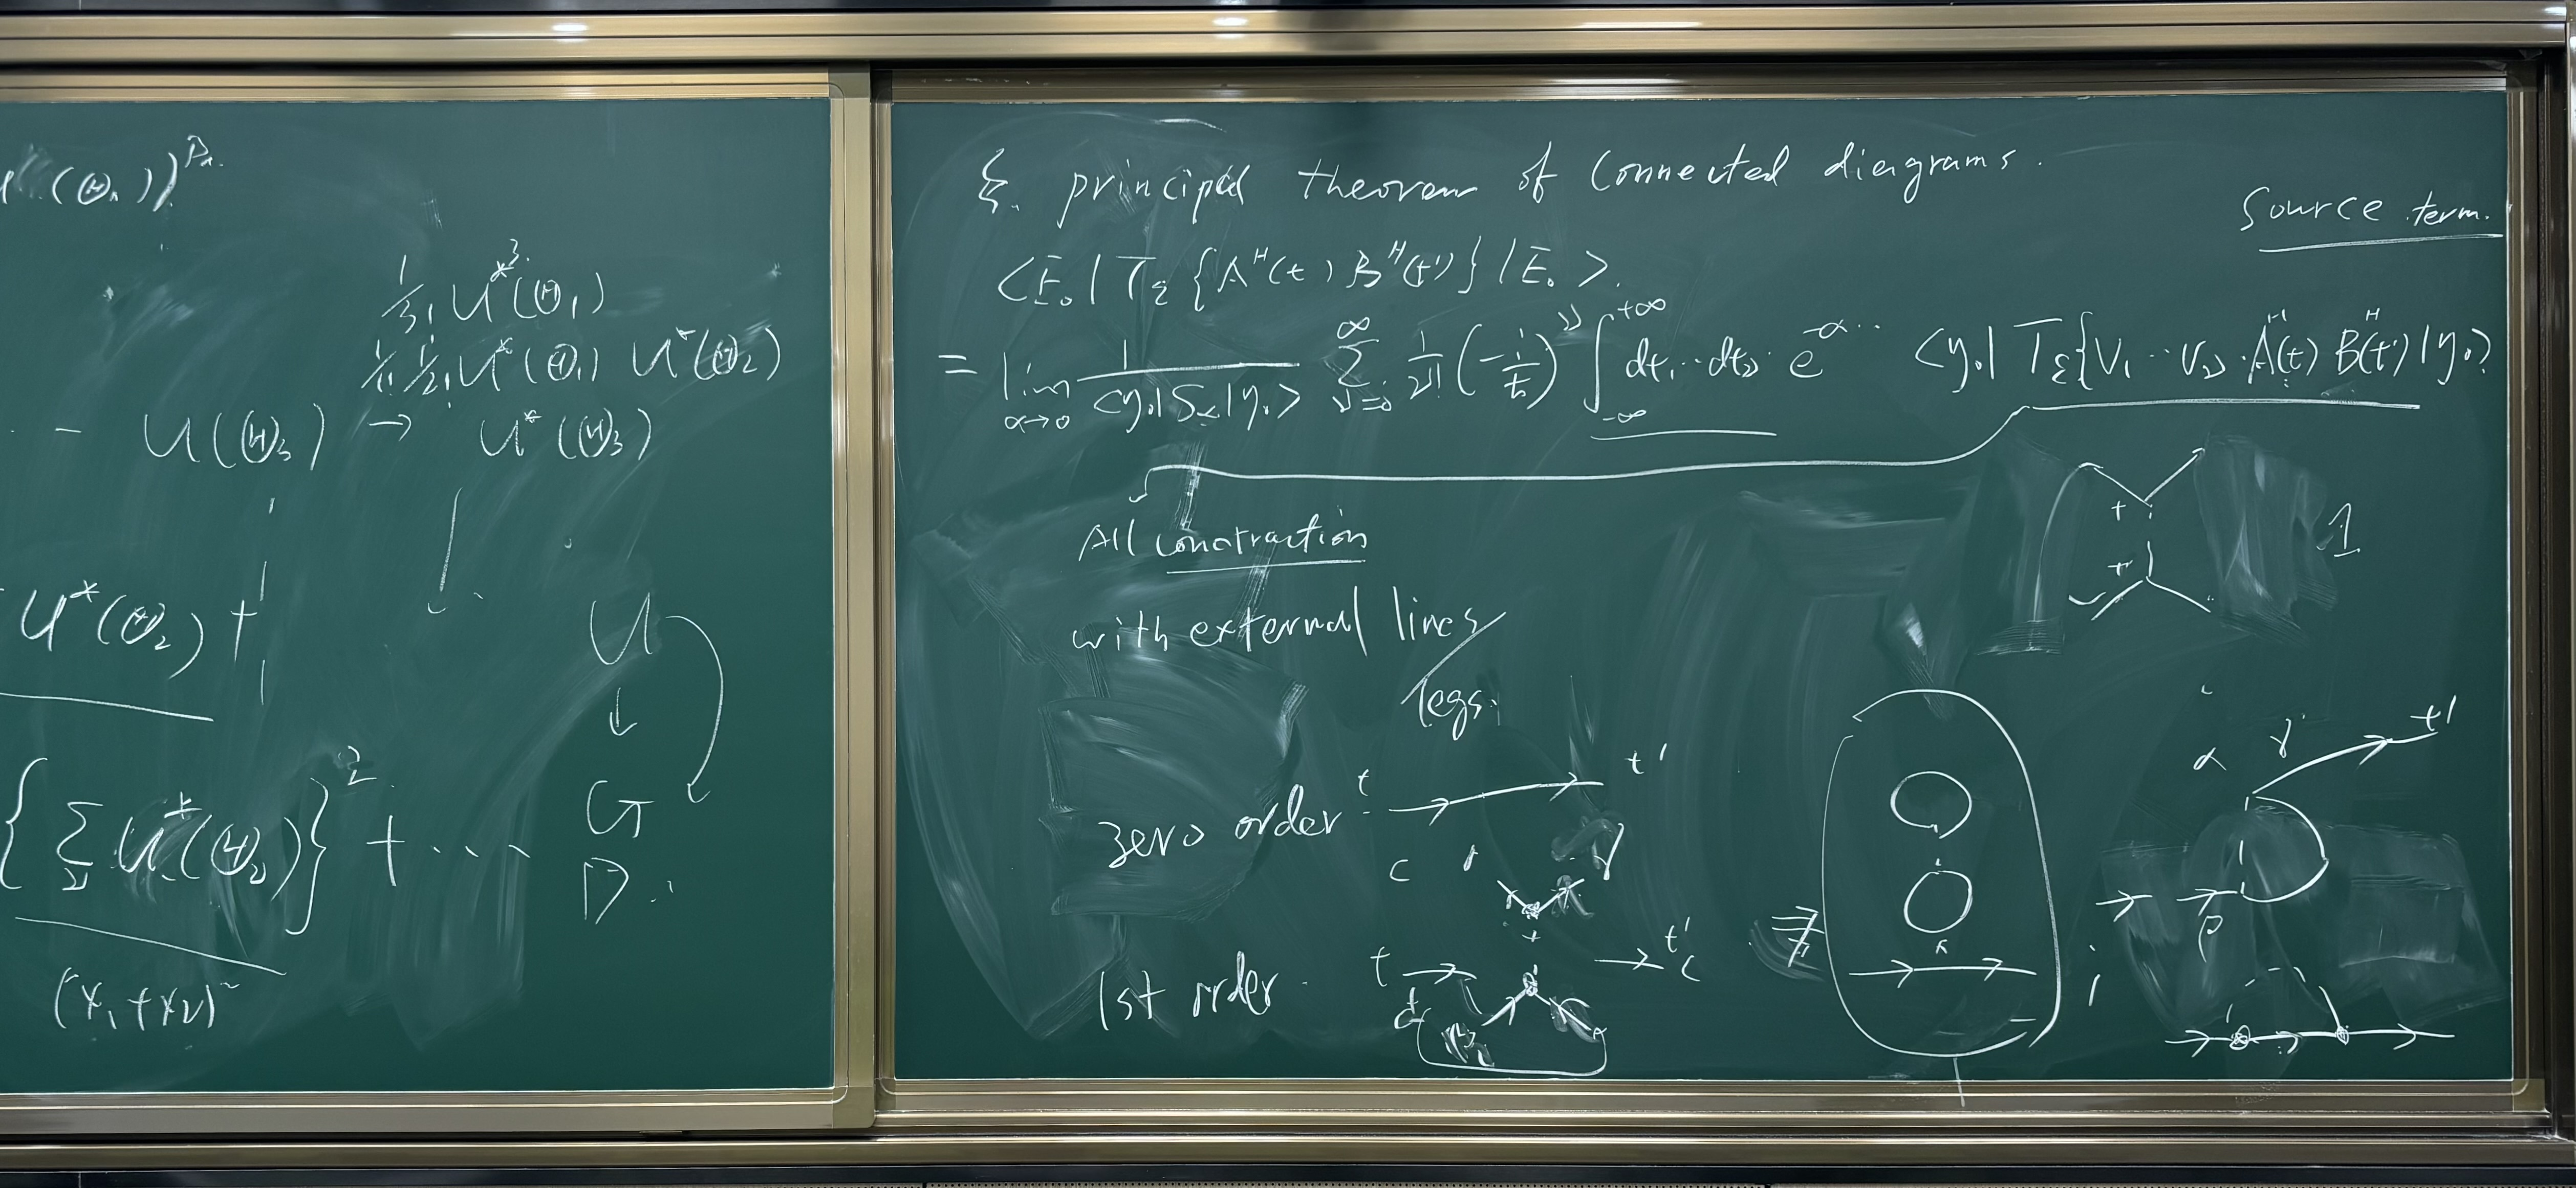
\includegraphics[width = \linewidth]{./media/feynmann12.jpeg}
\end{center}

\subsection{Principal theorems of connected diagrams}

\begin{enumext}
  \item ``Open'' diagrams: with external legs $U(p_\nu)$
  \item ``Closed'' diagrams: no external legs.
  \[
    U(\Theta_\nu) = U(p_0) \exp\ab\{\sum_\gamma U^\dagger(\Theta_\nu)\}
    \Rightarrow \ab(\sum_{p_0} U(p_0))
    \exp\ab\{\sum_\gamma U^\dagger(\Theta_\nu)\}
  \]
  $\braket<\eta_0|S_\alpha|\eta_0>\big|_{\alpha\to0} \upe^{\iu\cdots/\alpha}$
  cancels the Feynman diagram.
\end{enumext}

\subsection{Coleman replica trick via $\mathtt S$-matrix with source}

\[
  \ln S = \lim_{n\to} \ab(\frac{S^n - 1}{n})
\]
where $(S_i[\bar\alpha,\alpha])^n
  = \ab(\braket<\eta_0|T_\epsilon\exp[-\iu\int\d t \sum V
  + \underset{\alpha_{c^\dagger}c^\dagger + \bar\alpha_cc}
      {\underline{\text{Source terms}}}]|\eta_0>)^n$. It can be expanded as
\begin{center}
  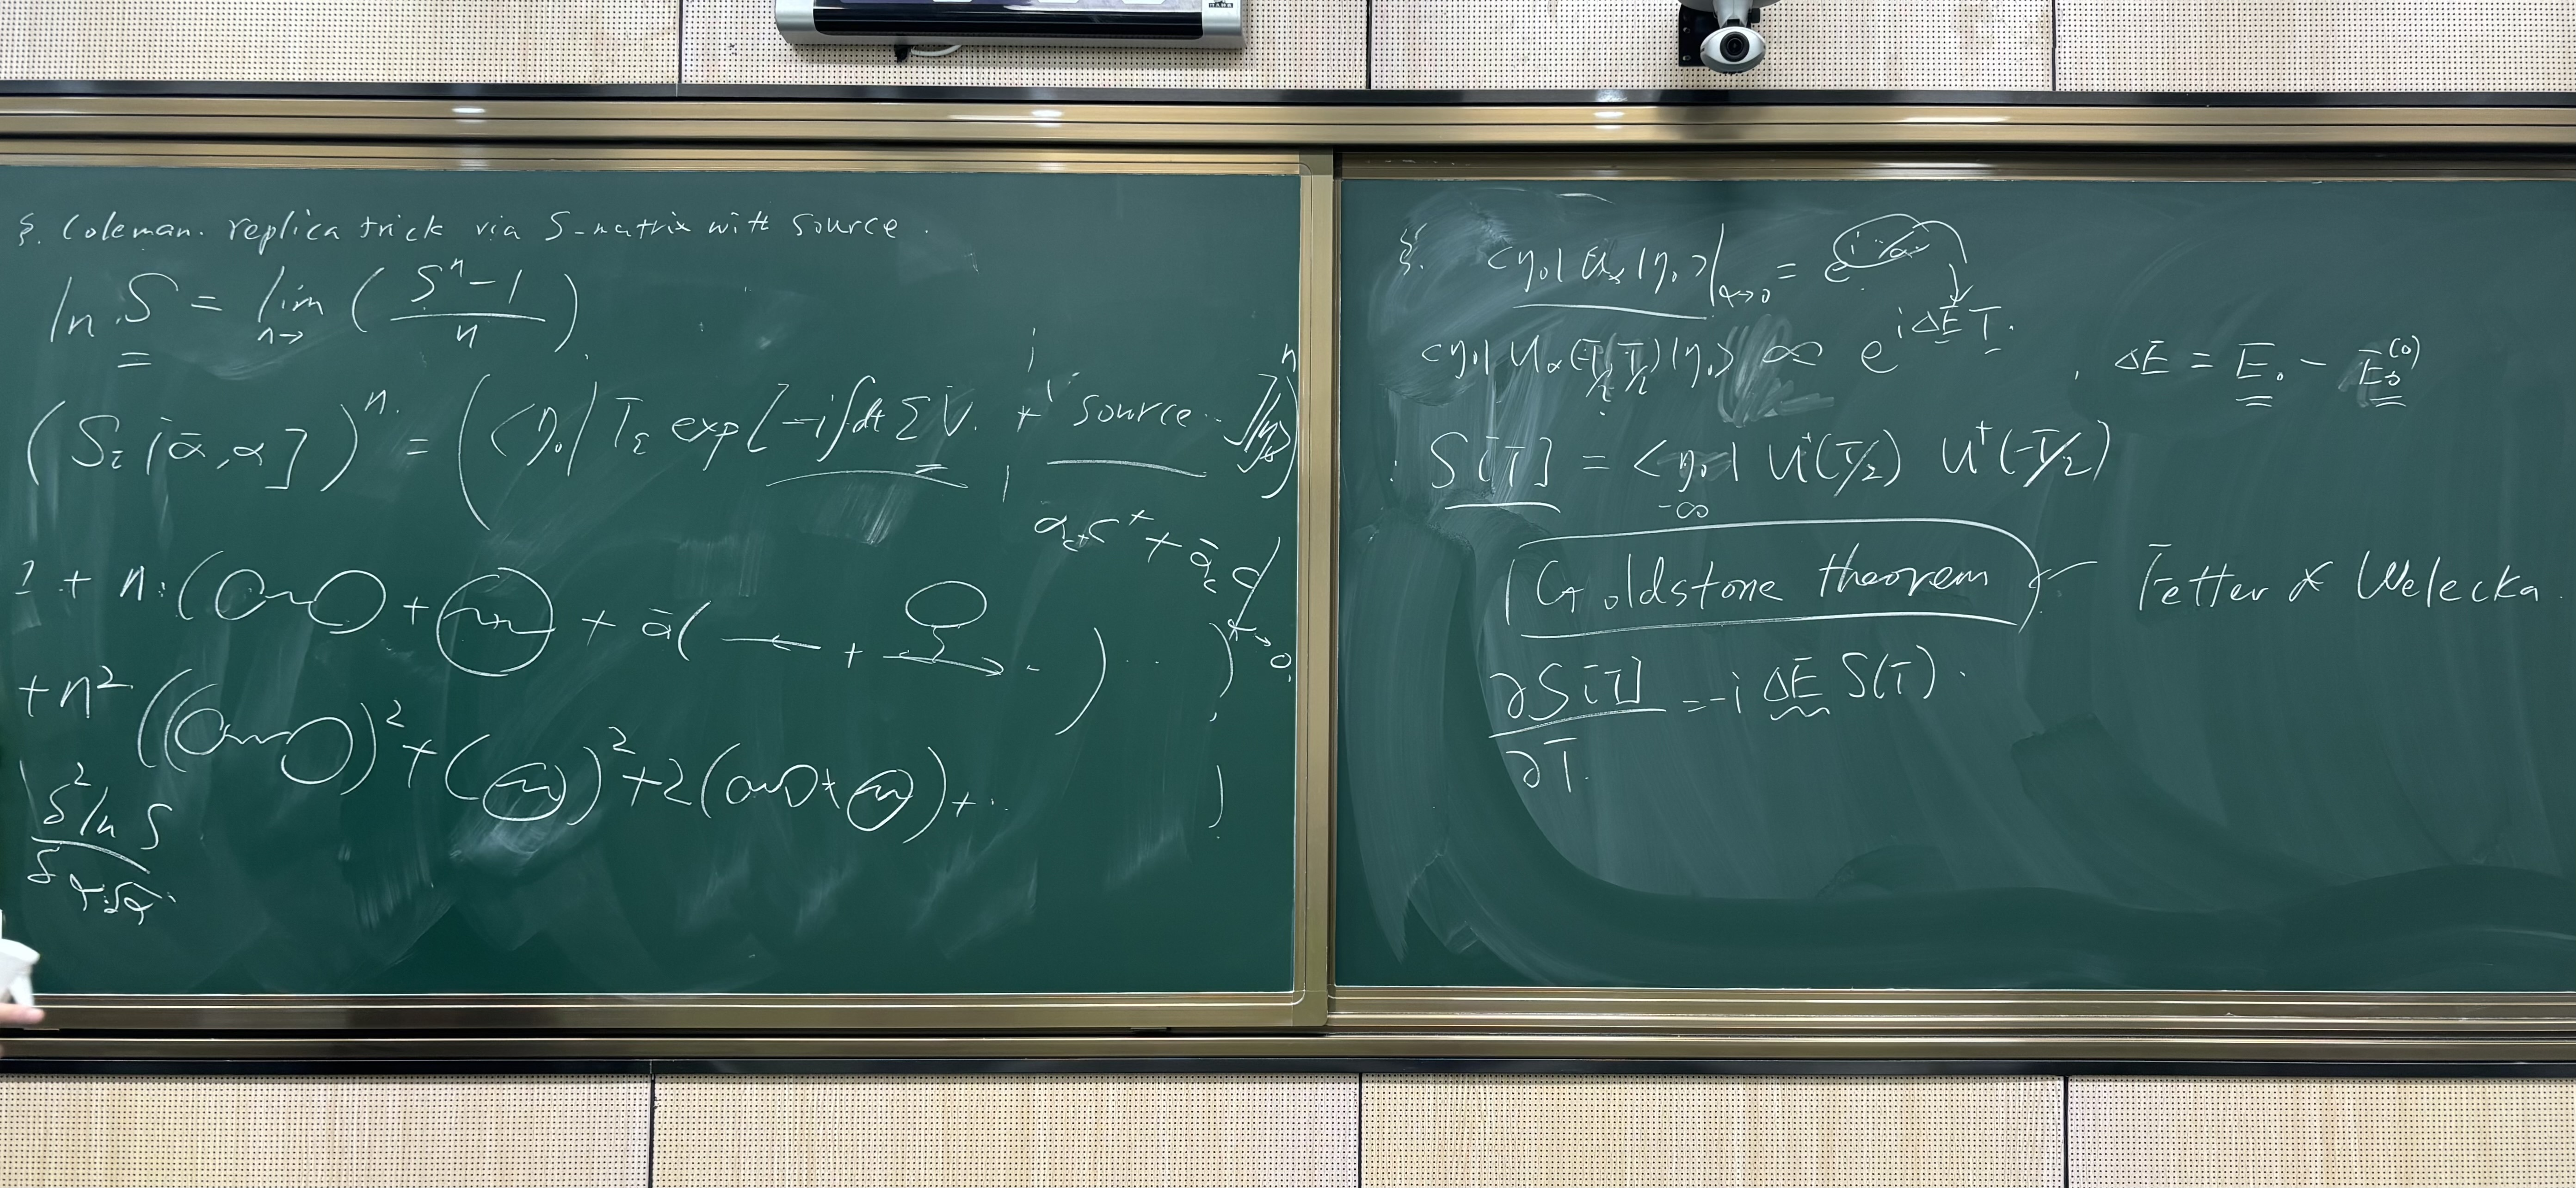
\includegraphics[width = \linewidth]{./media/feynmann13.jpeg}
\end{center}
\[
  \braket<\eta_0|U_\alpha|\eta_0>\big|_{\alpha\to0} = \upe^{\iu\cdots/\alpha},
  \quad
  \braket<\eta_0|U_\alpha(-T/\iu,T/\iu)|\eta_0> \propto \upe^{\iu\Delta ET}
\]
where $\Delta E = E_0 - E_0^{(0)}$.
If we consider a finite $T$: Goldstone theorem (Fetter \& Welecka).
\[
  S[T] = \braket<\eta_0|U^\dagger(T/2) U^\dagger(-T/2)|\eta_0>
\]
The derivative
\[
  \pdv{S[T]}{T} = -\iu\Delta ES(T).
\]

\subsection{Feynman diagram in momentum space}

\begin{center}
  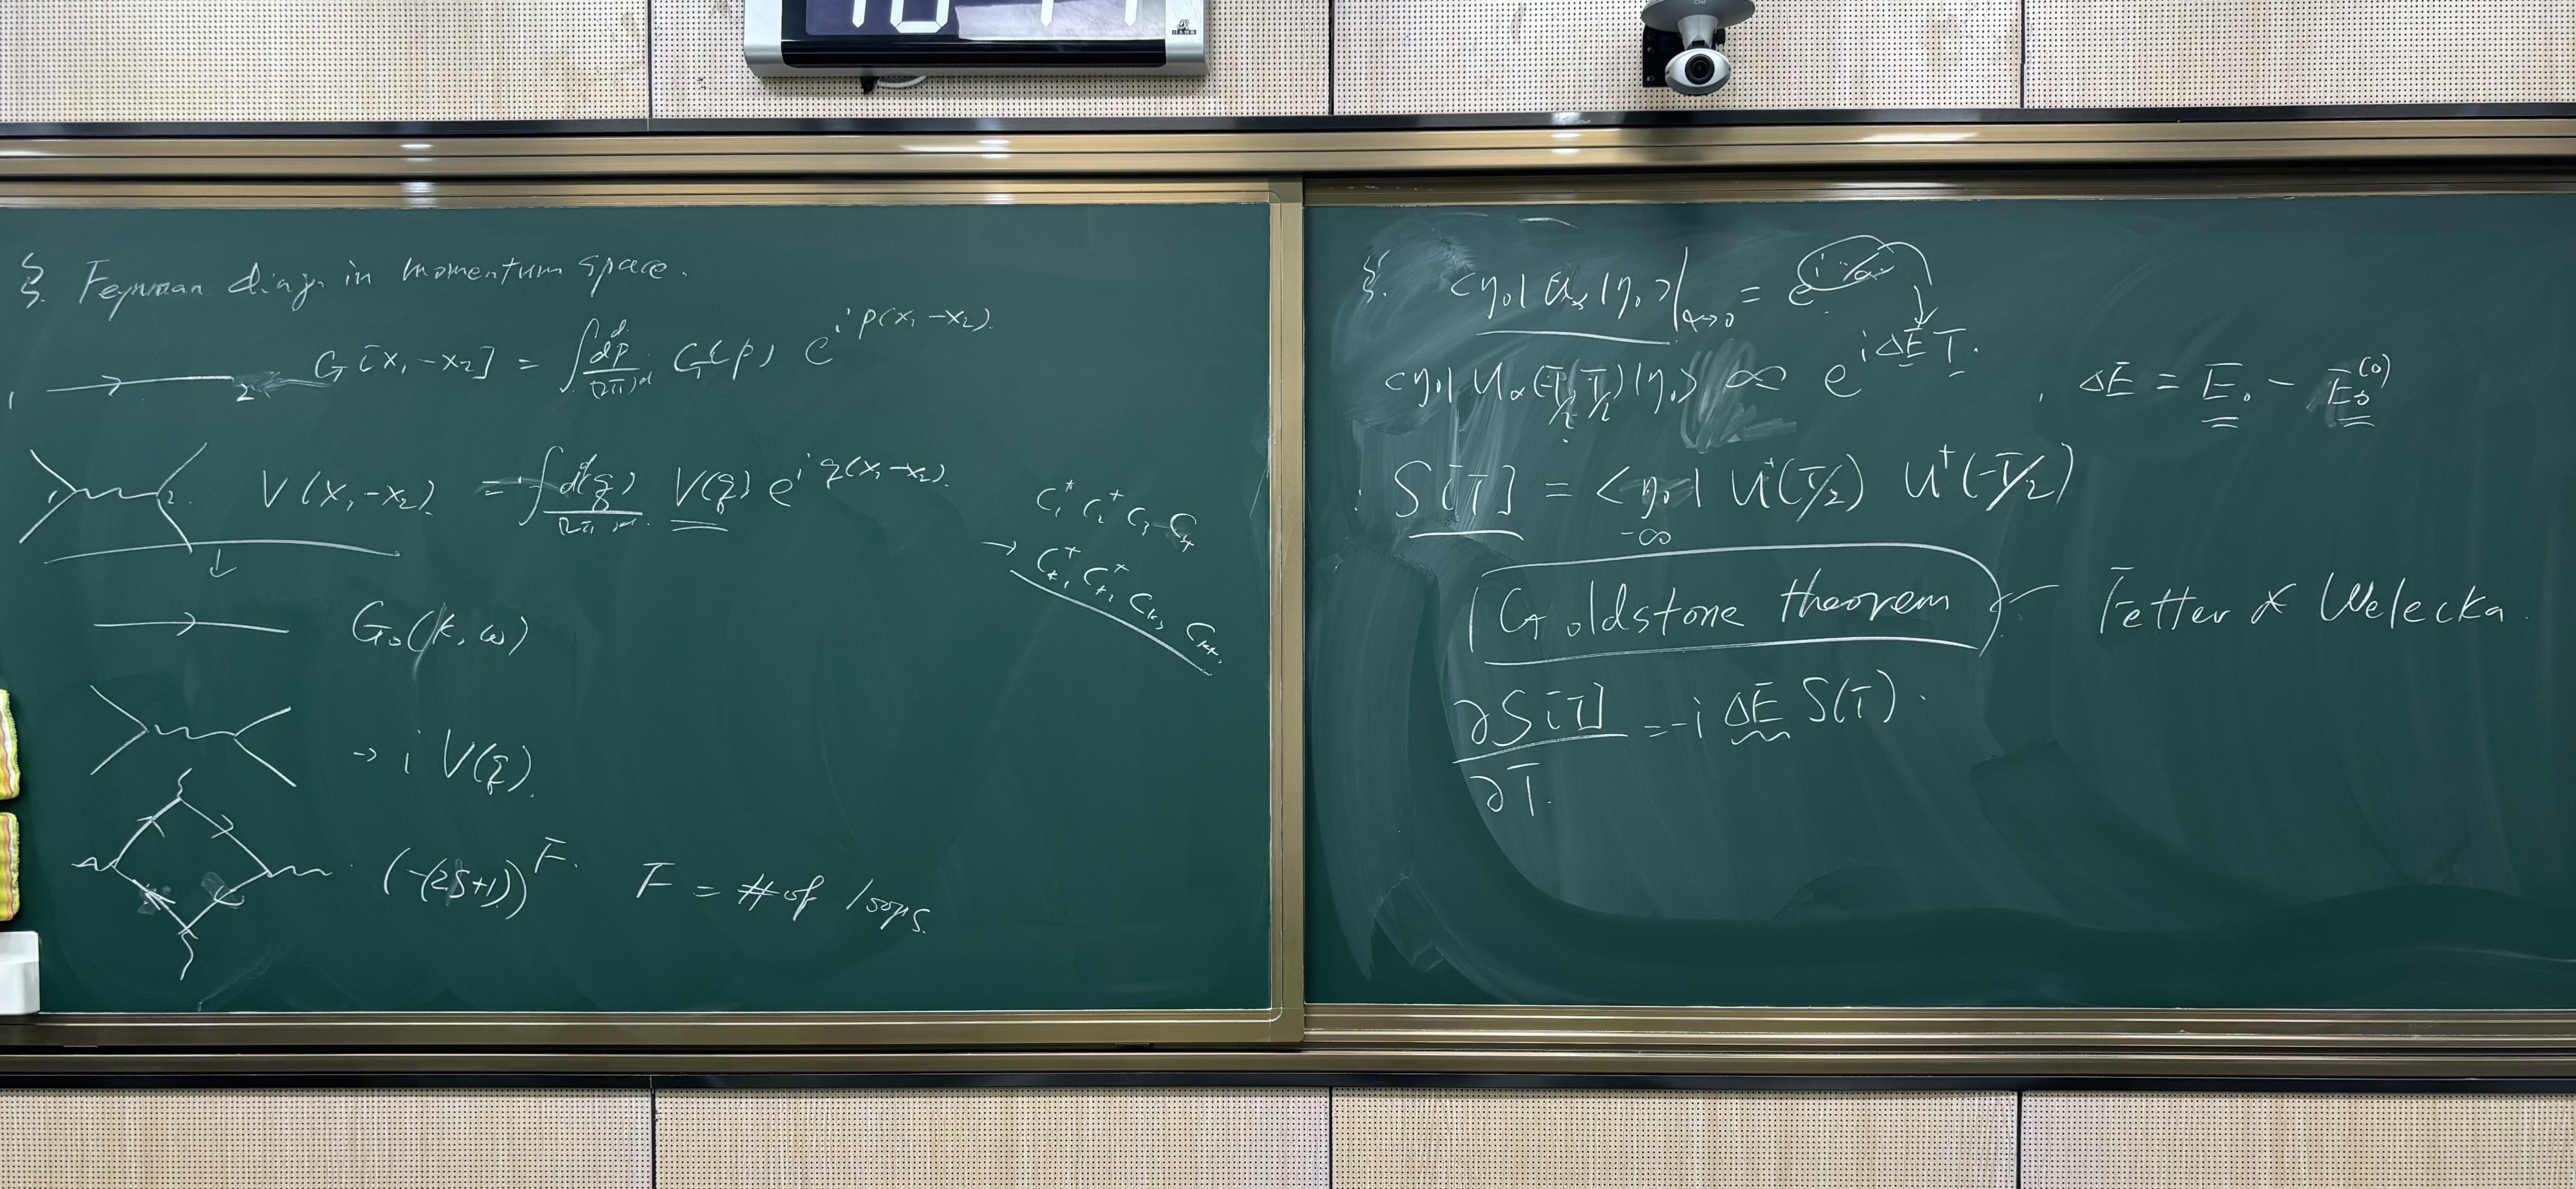
\includegraphics[width = \linewidth]{./media/feynmann14.jpeg}
\end{center}

\subsection{Single particle Green's function}

Diagrammatic expansion of Green's function
\begin{center}
  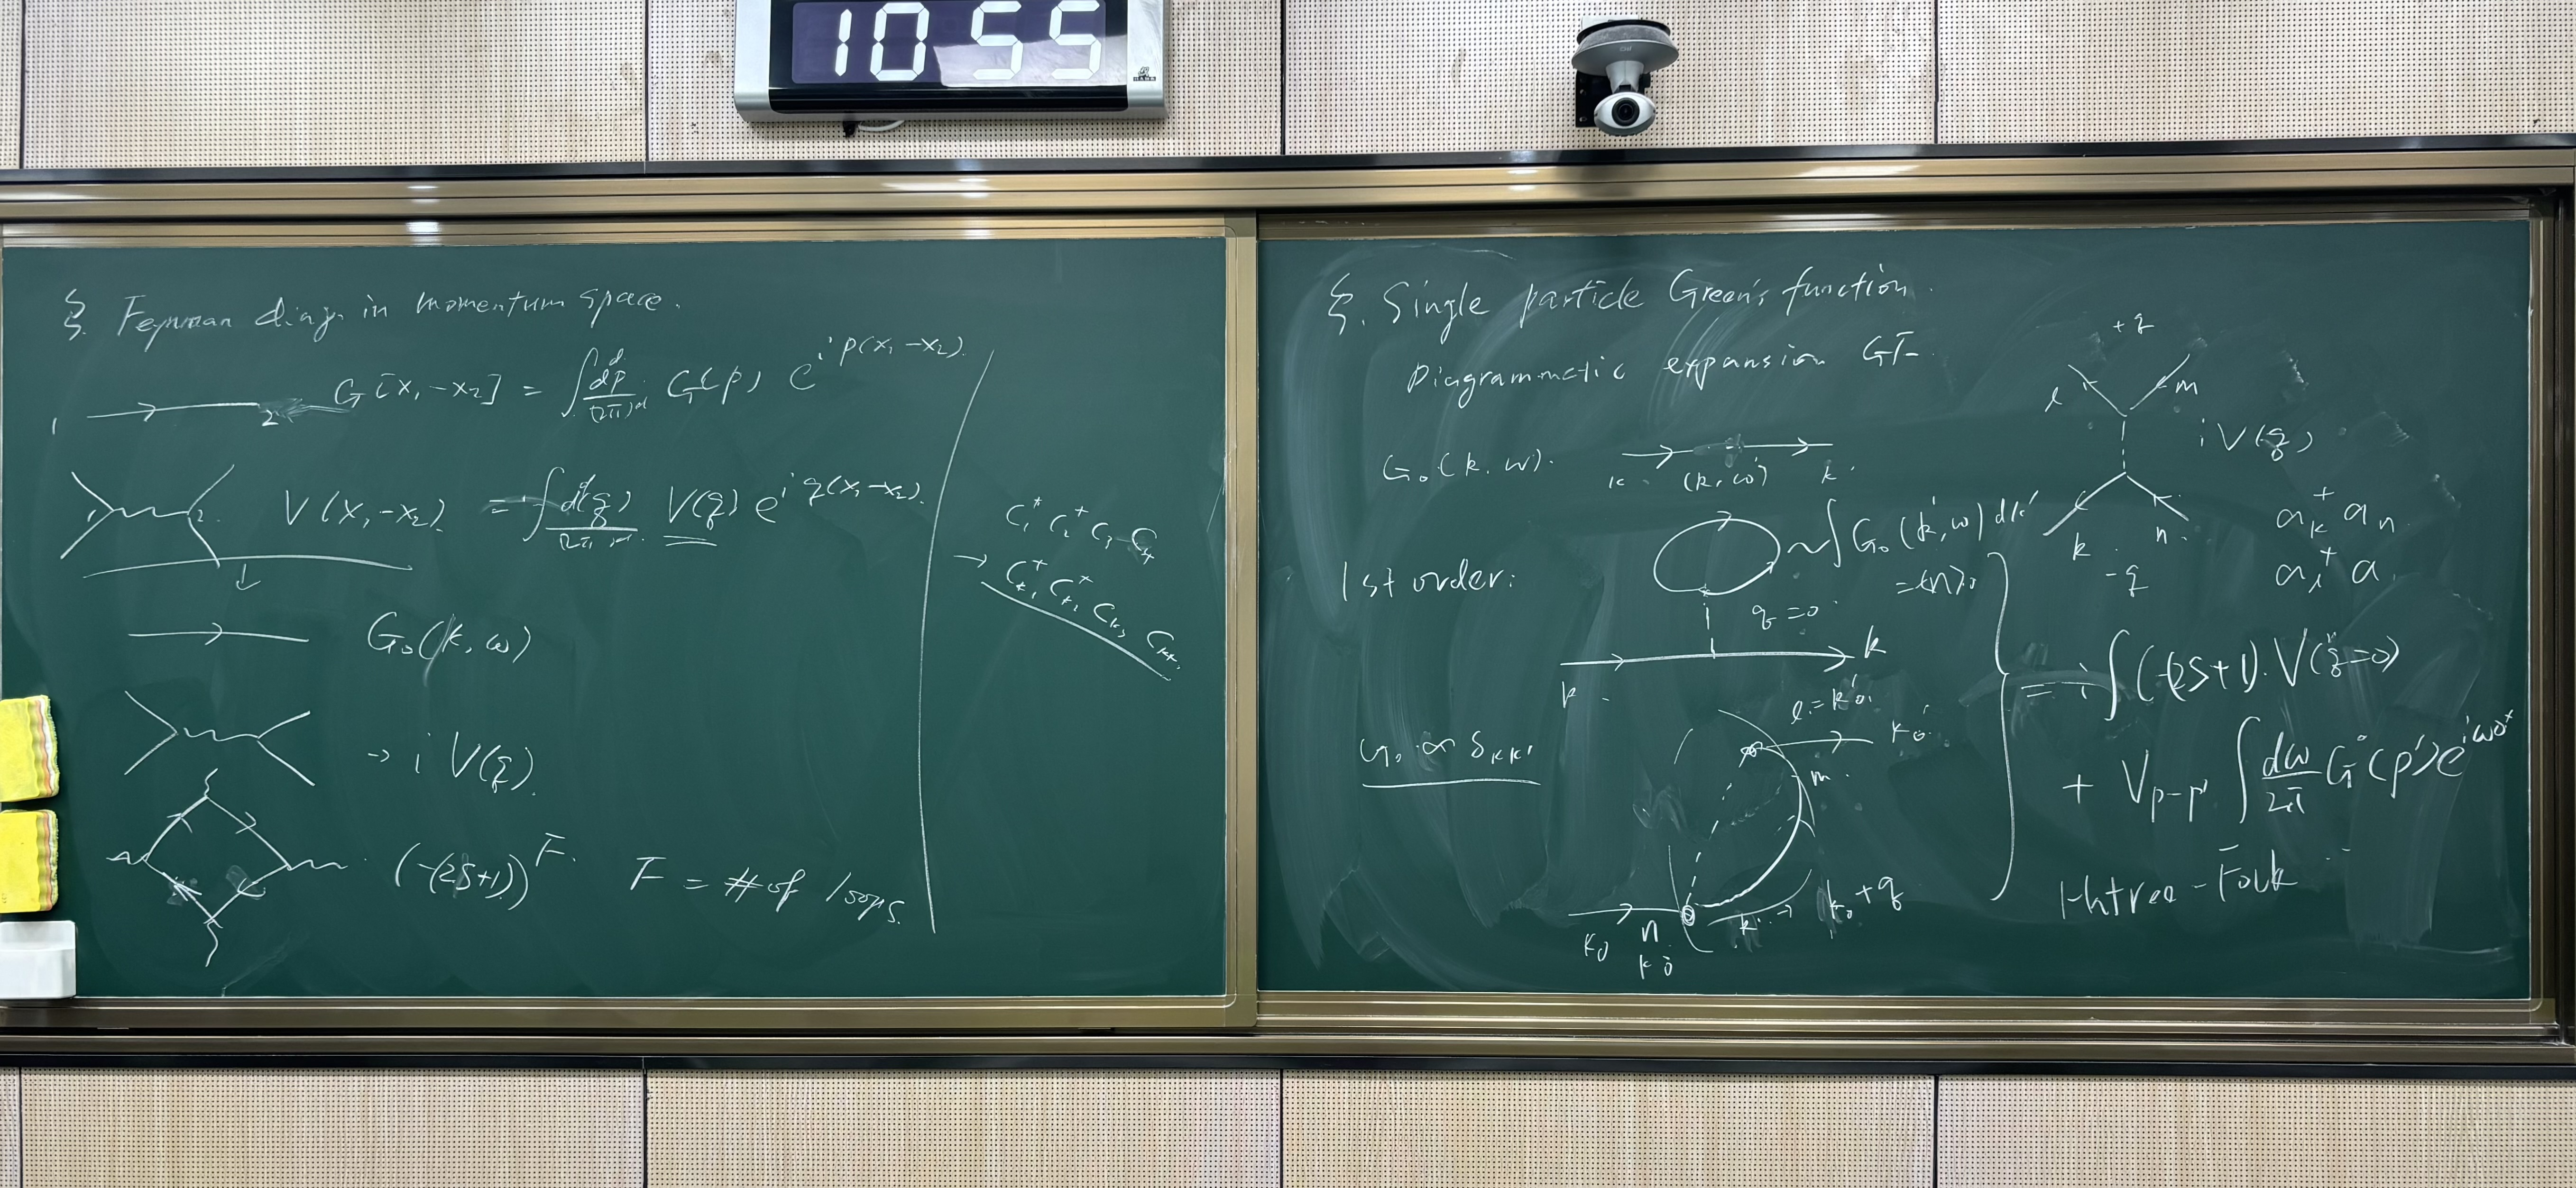
\includegraphics[width = \linewidth]{./media/feynmann15.jpeg}
\end{center}
\[
  \int \d q \braket<\eta_0|T_\epsilon(
    \wick{\c2 c_{k_0}^\dagger(\omega) \c1 c_{k_0}(\omega') V_q
          \c1 a_k^\dagger \c1 a_n \c1 a_l^\dagger \c2 a_m }
  )>
\]
where $k - n = l - m = q$.
\[
  \wick{\c1 G^0(k_0,\omega) \c3\delta_{k_0,k} \c2 \delta_{k_0',m} \c1\delta_{nl}
      \c3 G_0(\c2 k_n)}
\]
\begin{center}
  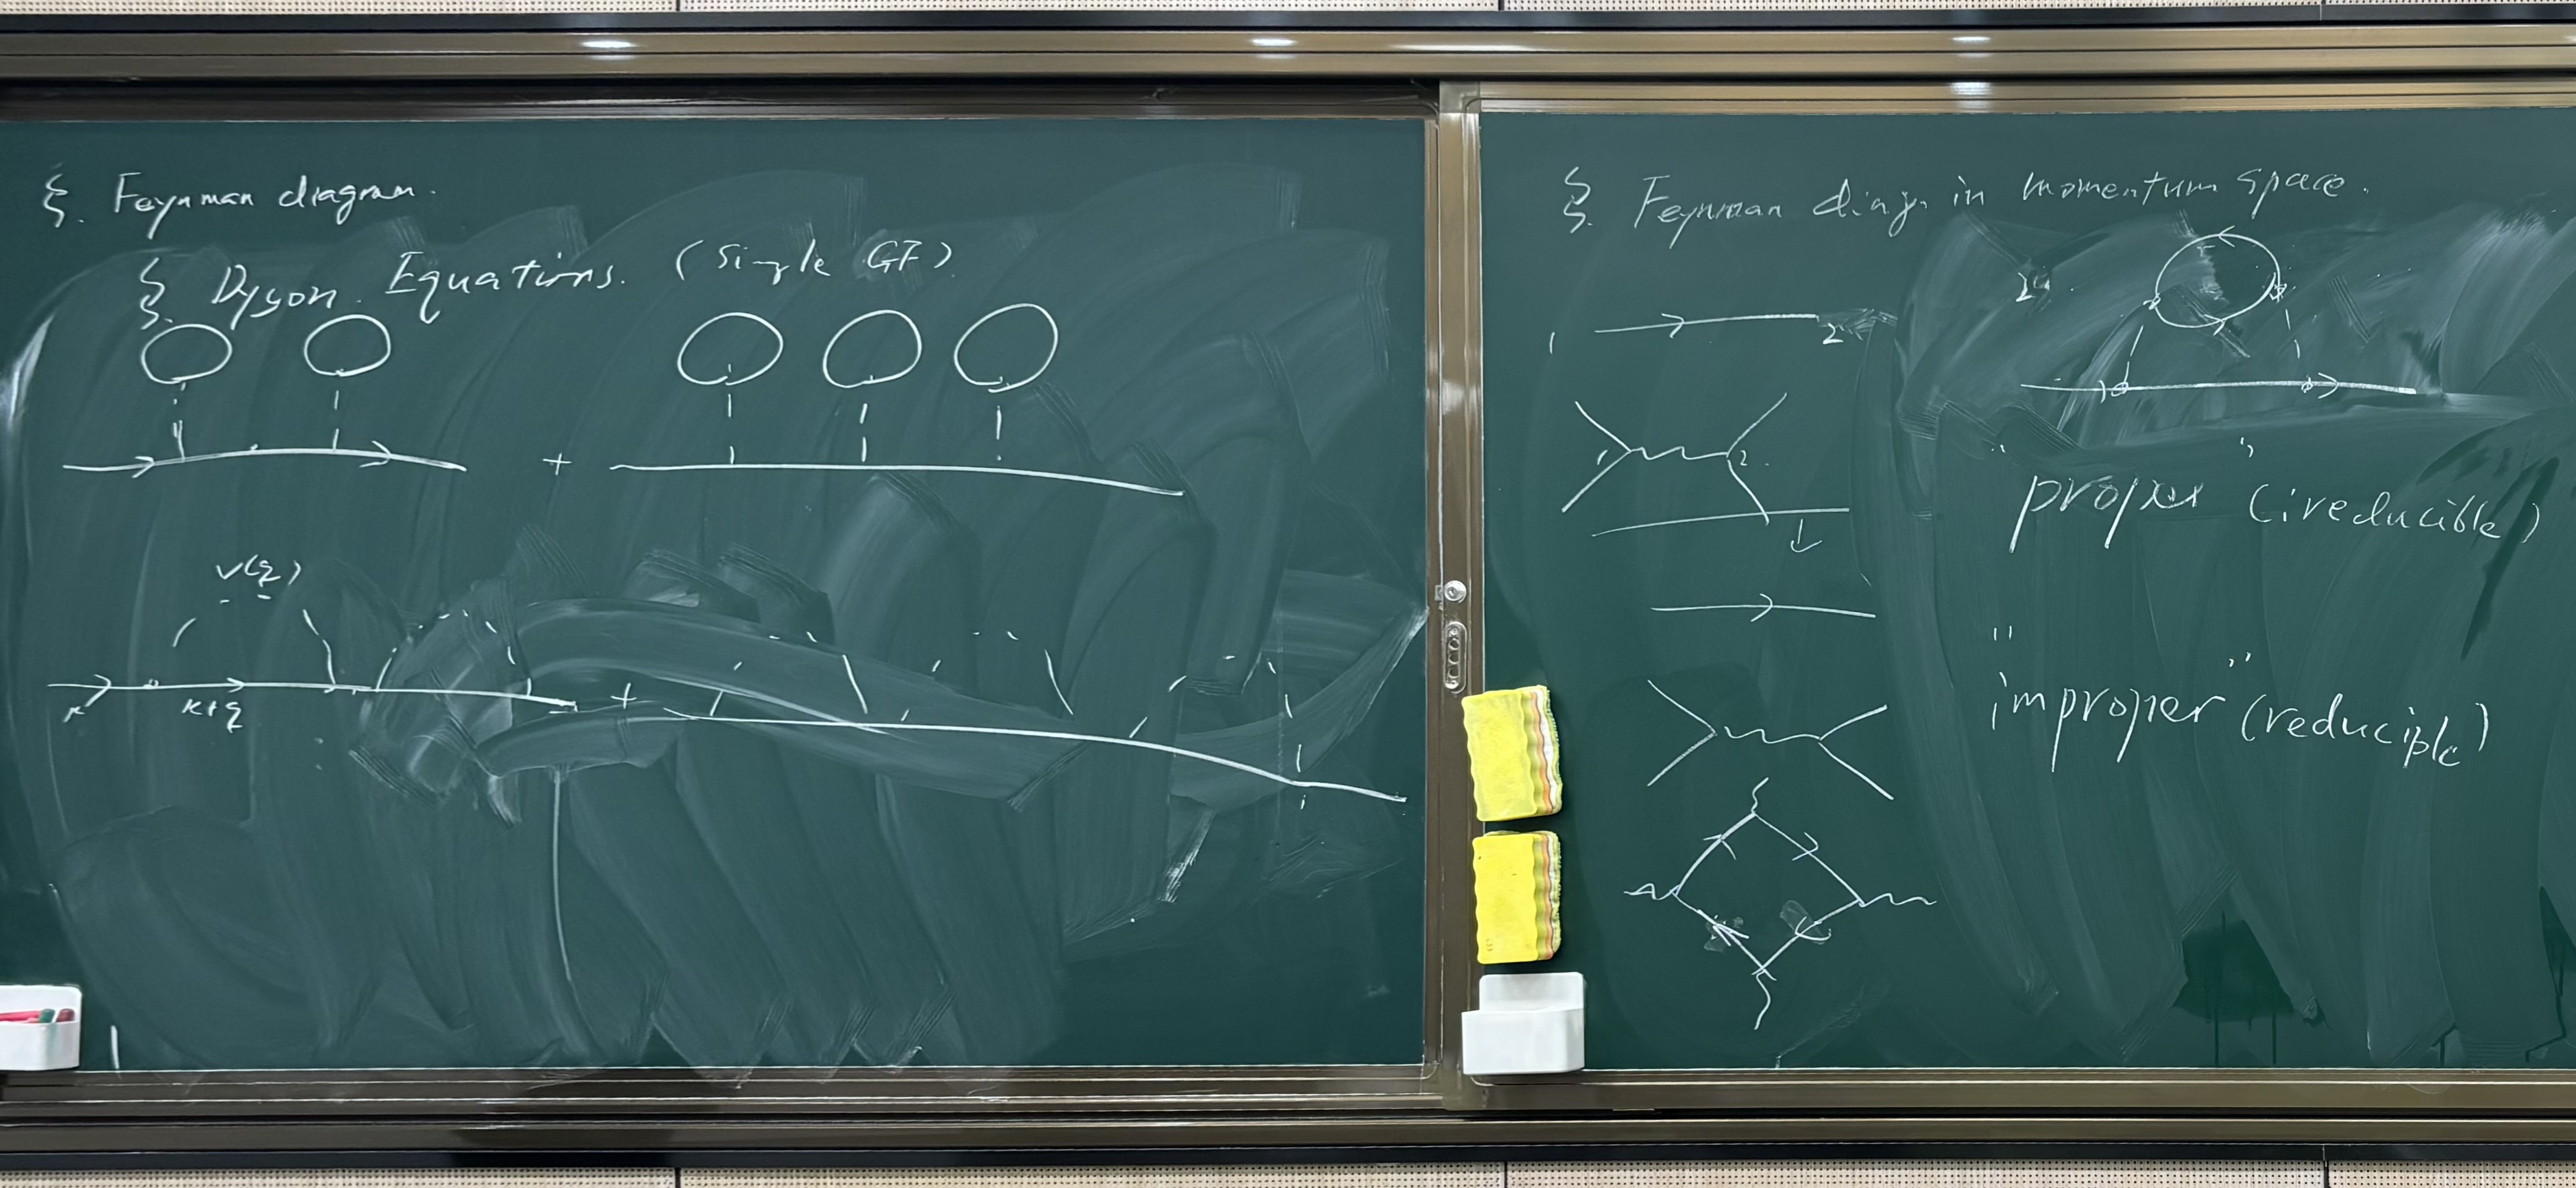
\includegraphics[width = \linewidth]{./media/feynmann16.jpeg}
\end{center}
Define the self-energy
\begin{center}
  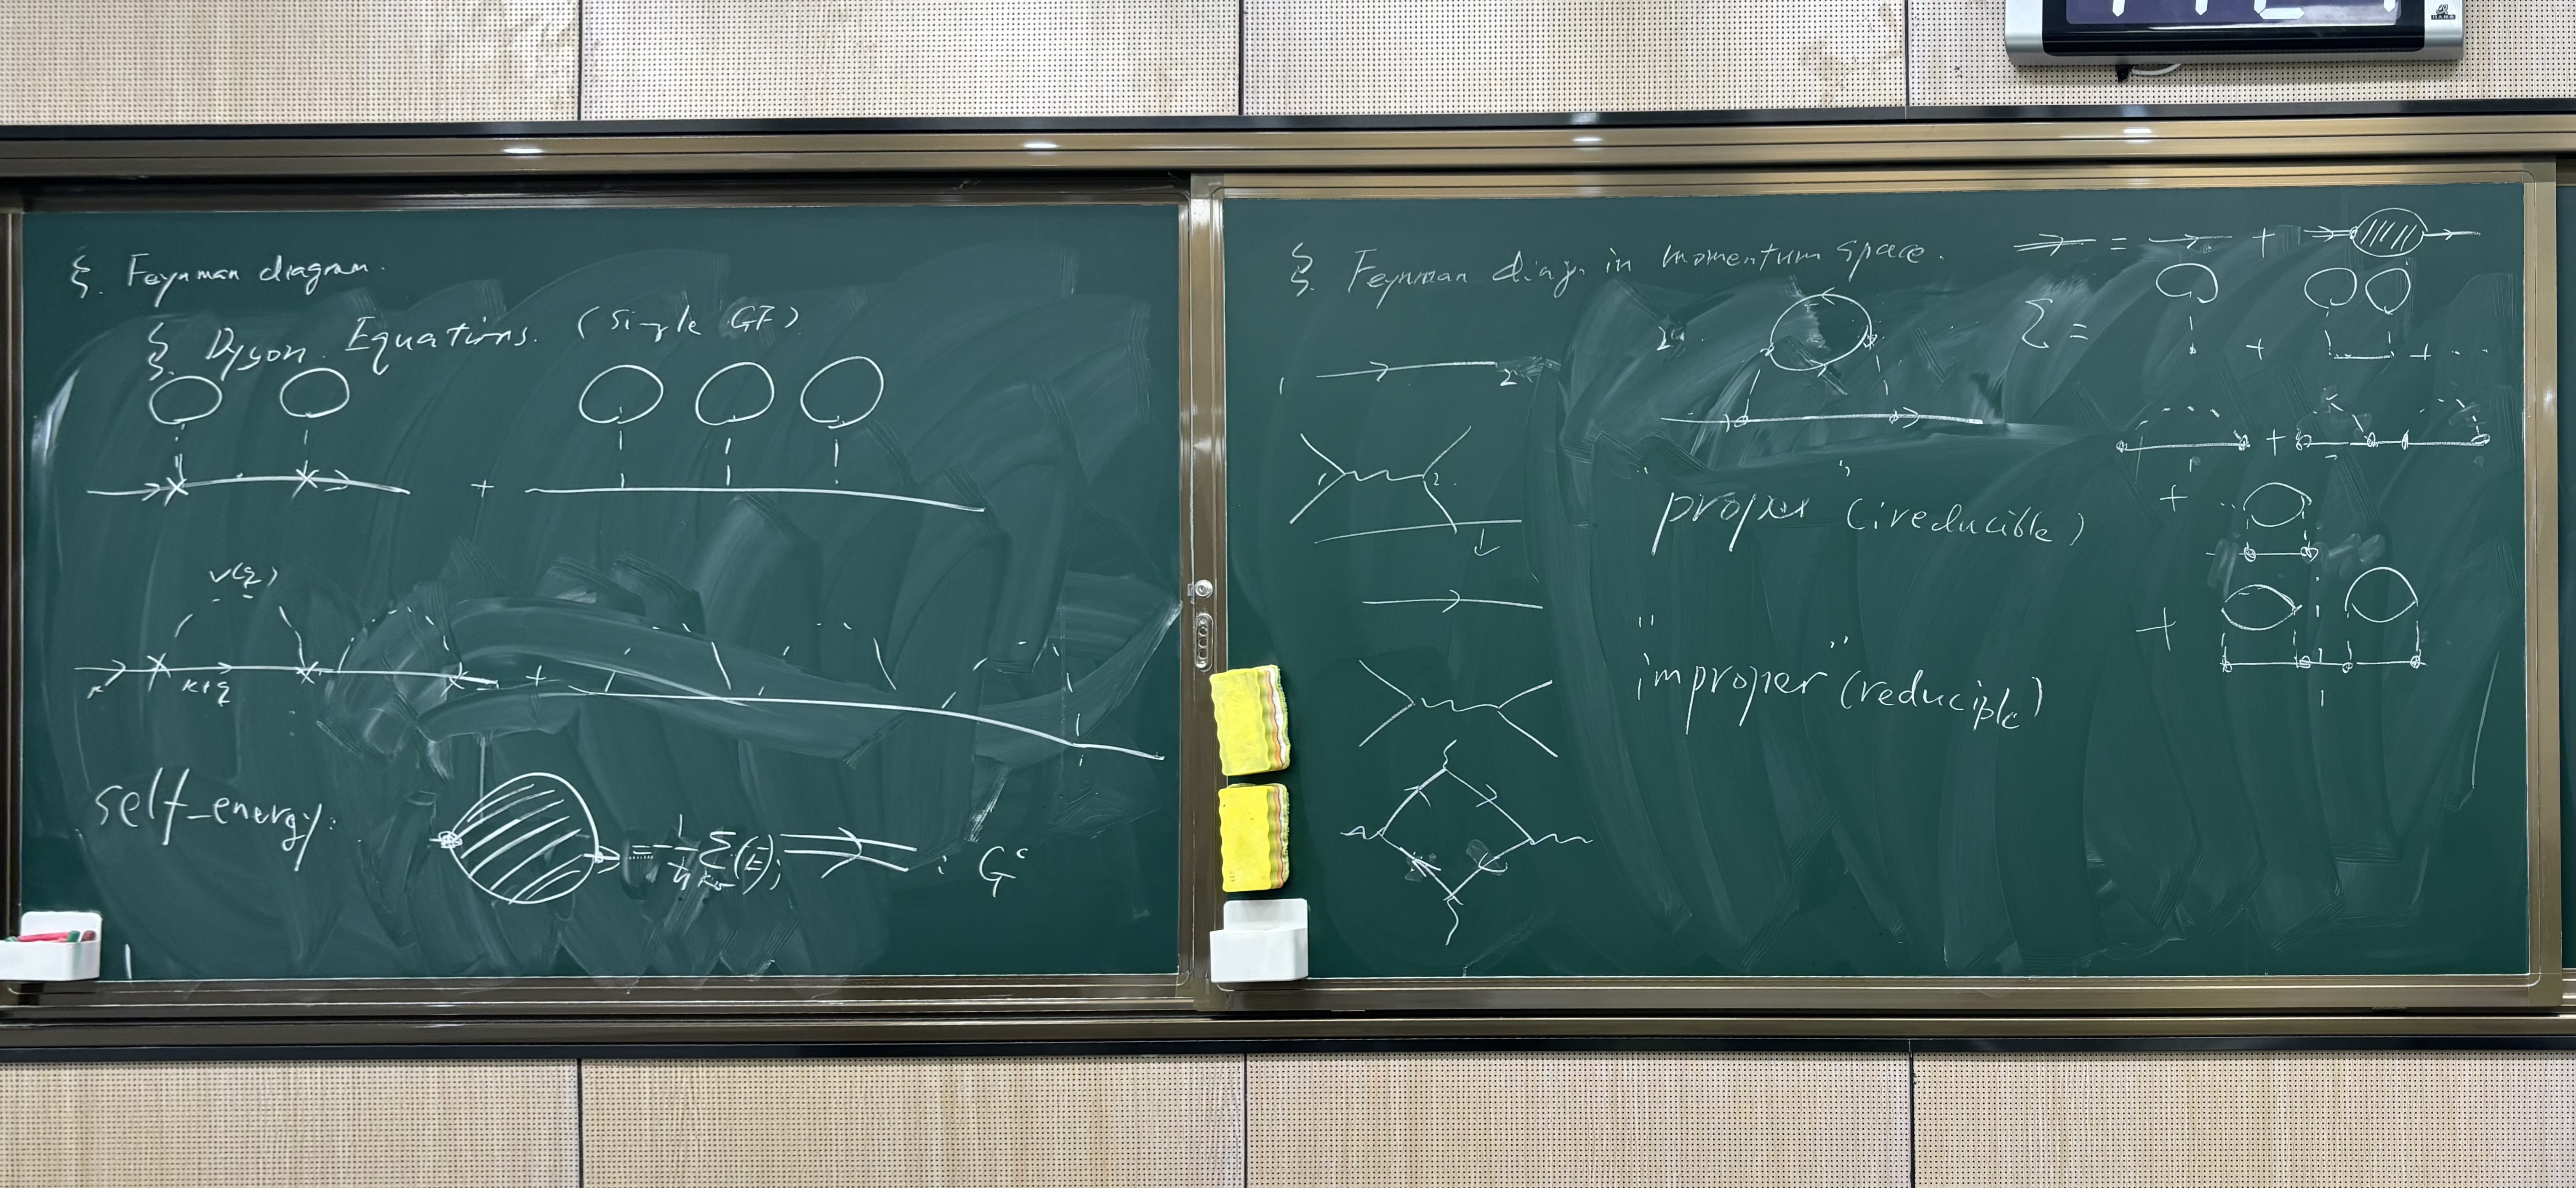
\includegraphics[width = \linewidth]{./media/feynmann17.jpeg}
\end{center}
Proper/ireducible =
cannot be decomposed into independent (repeated lower order diagram)
contribution by ``removal of one/single propagating ling''.
Get the Green's function from Dyson equation from Feynman diagram way
\[
  G = \frac1{E - \epsilon_0 - \Sigma}
\]
\begin{center}
  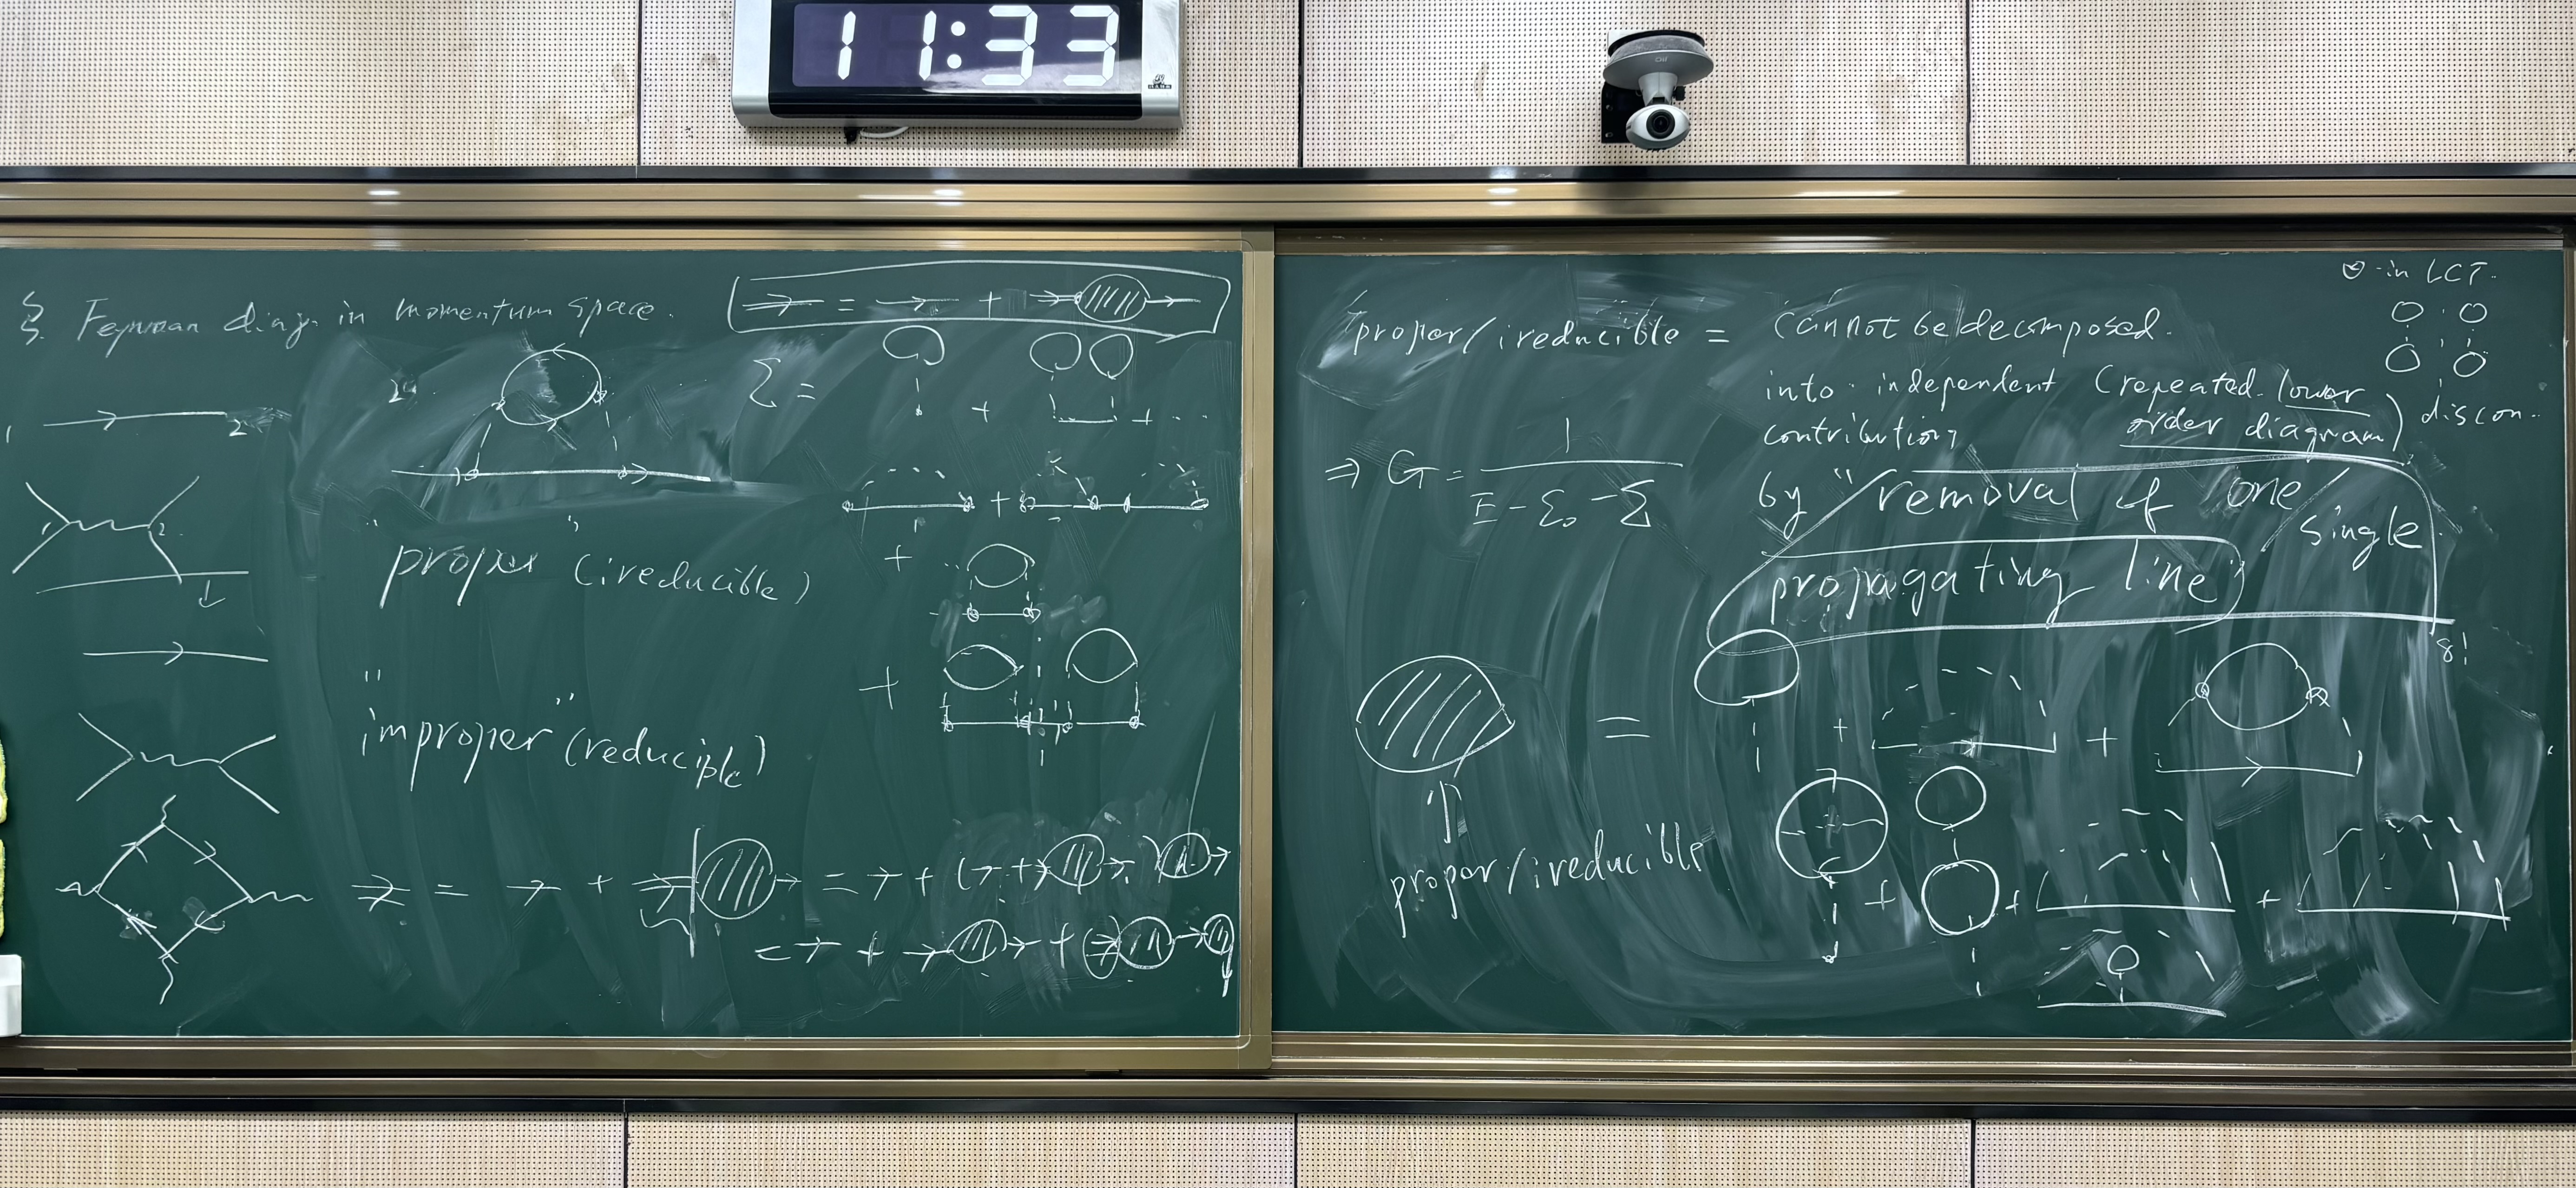
\includegraphics[width = \linewidth]{./media/feynmann18.jpeg}
\end{center}

\section{Diagrammatic partial sums}

\subsection{Polarization propagator}

\begin{example}\leavevmode
  \[
    D_q(t,t') = \ab*<\braket<\rho_q(t);\rho_q^\dagger(t')>>
  \]
  where $\rho_q = \sum_{\sigma,k} a_k^\dagger a_{k+q}$,
  $\rho_q^\dagger(t) = \rho_{-q}(t)$.
  We can also have a singular bubble
  $\chi_c = \ab*<\braket<S^z S^\dagger>>
= -\braket<\rho_q(t)>\braket<\rho_q^\dagger(t')>$.
\end{example}
\begin{center}
  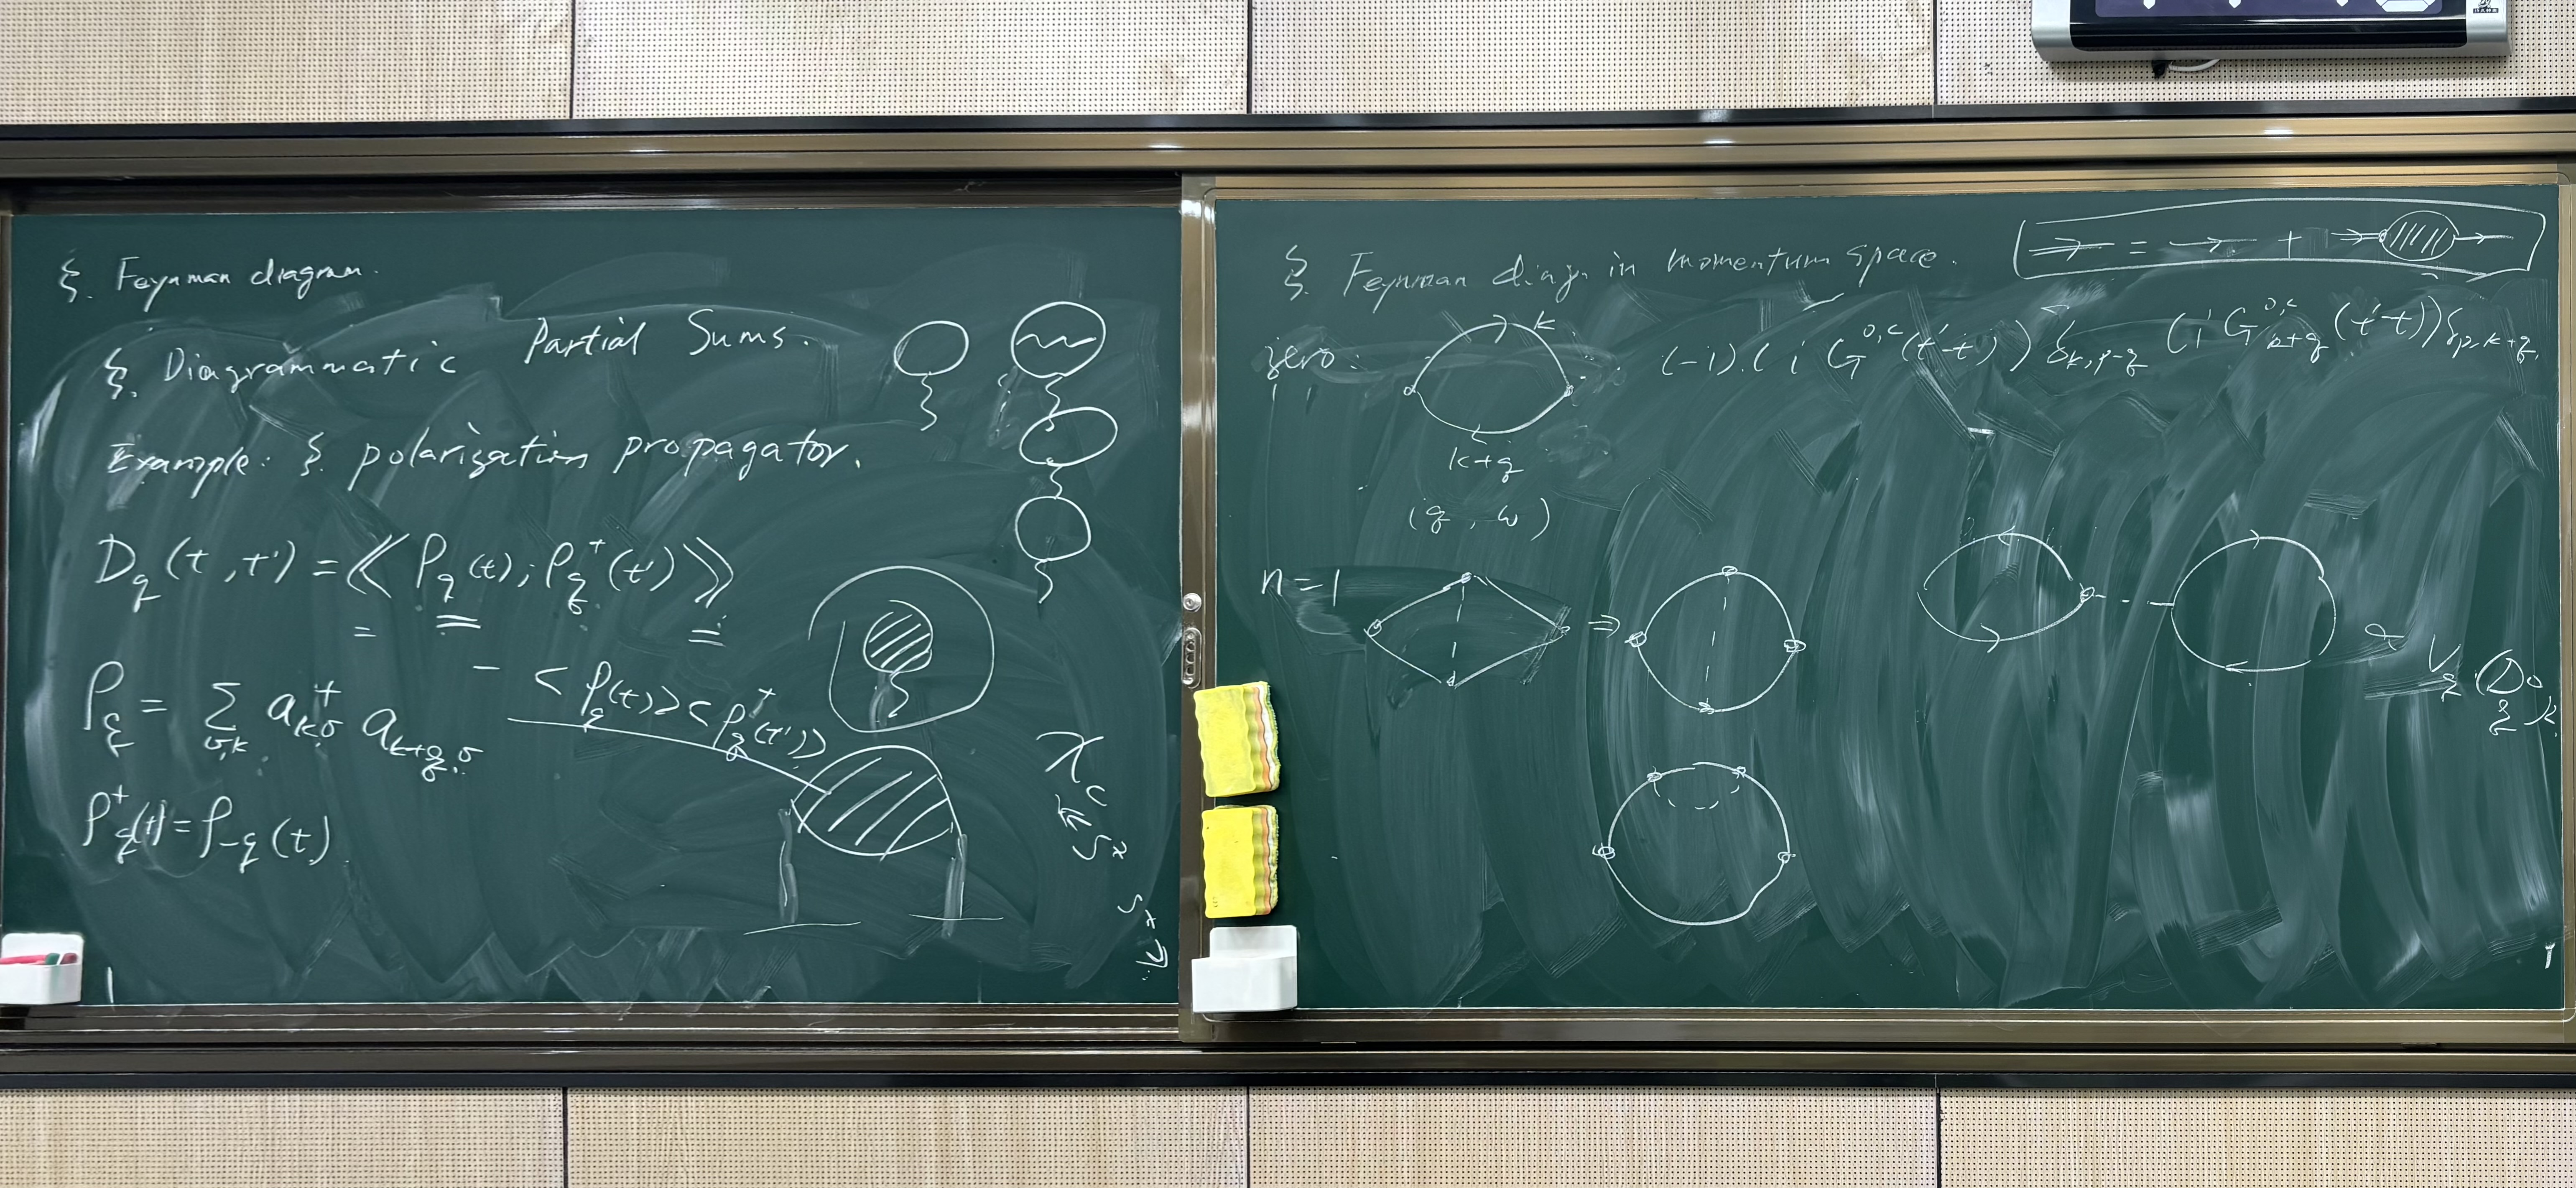
\includegraphics[width = \linewidth]{./media/feynmann19.jpeg}
\end{center}
By cutting vertex line
\begin{enumext}[columns = 2]
  \item Irreducible
  \item Reducible
\end{enumext}
\begin{center}
  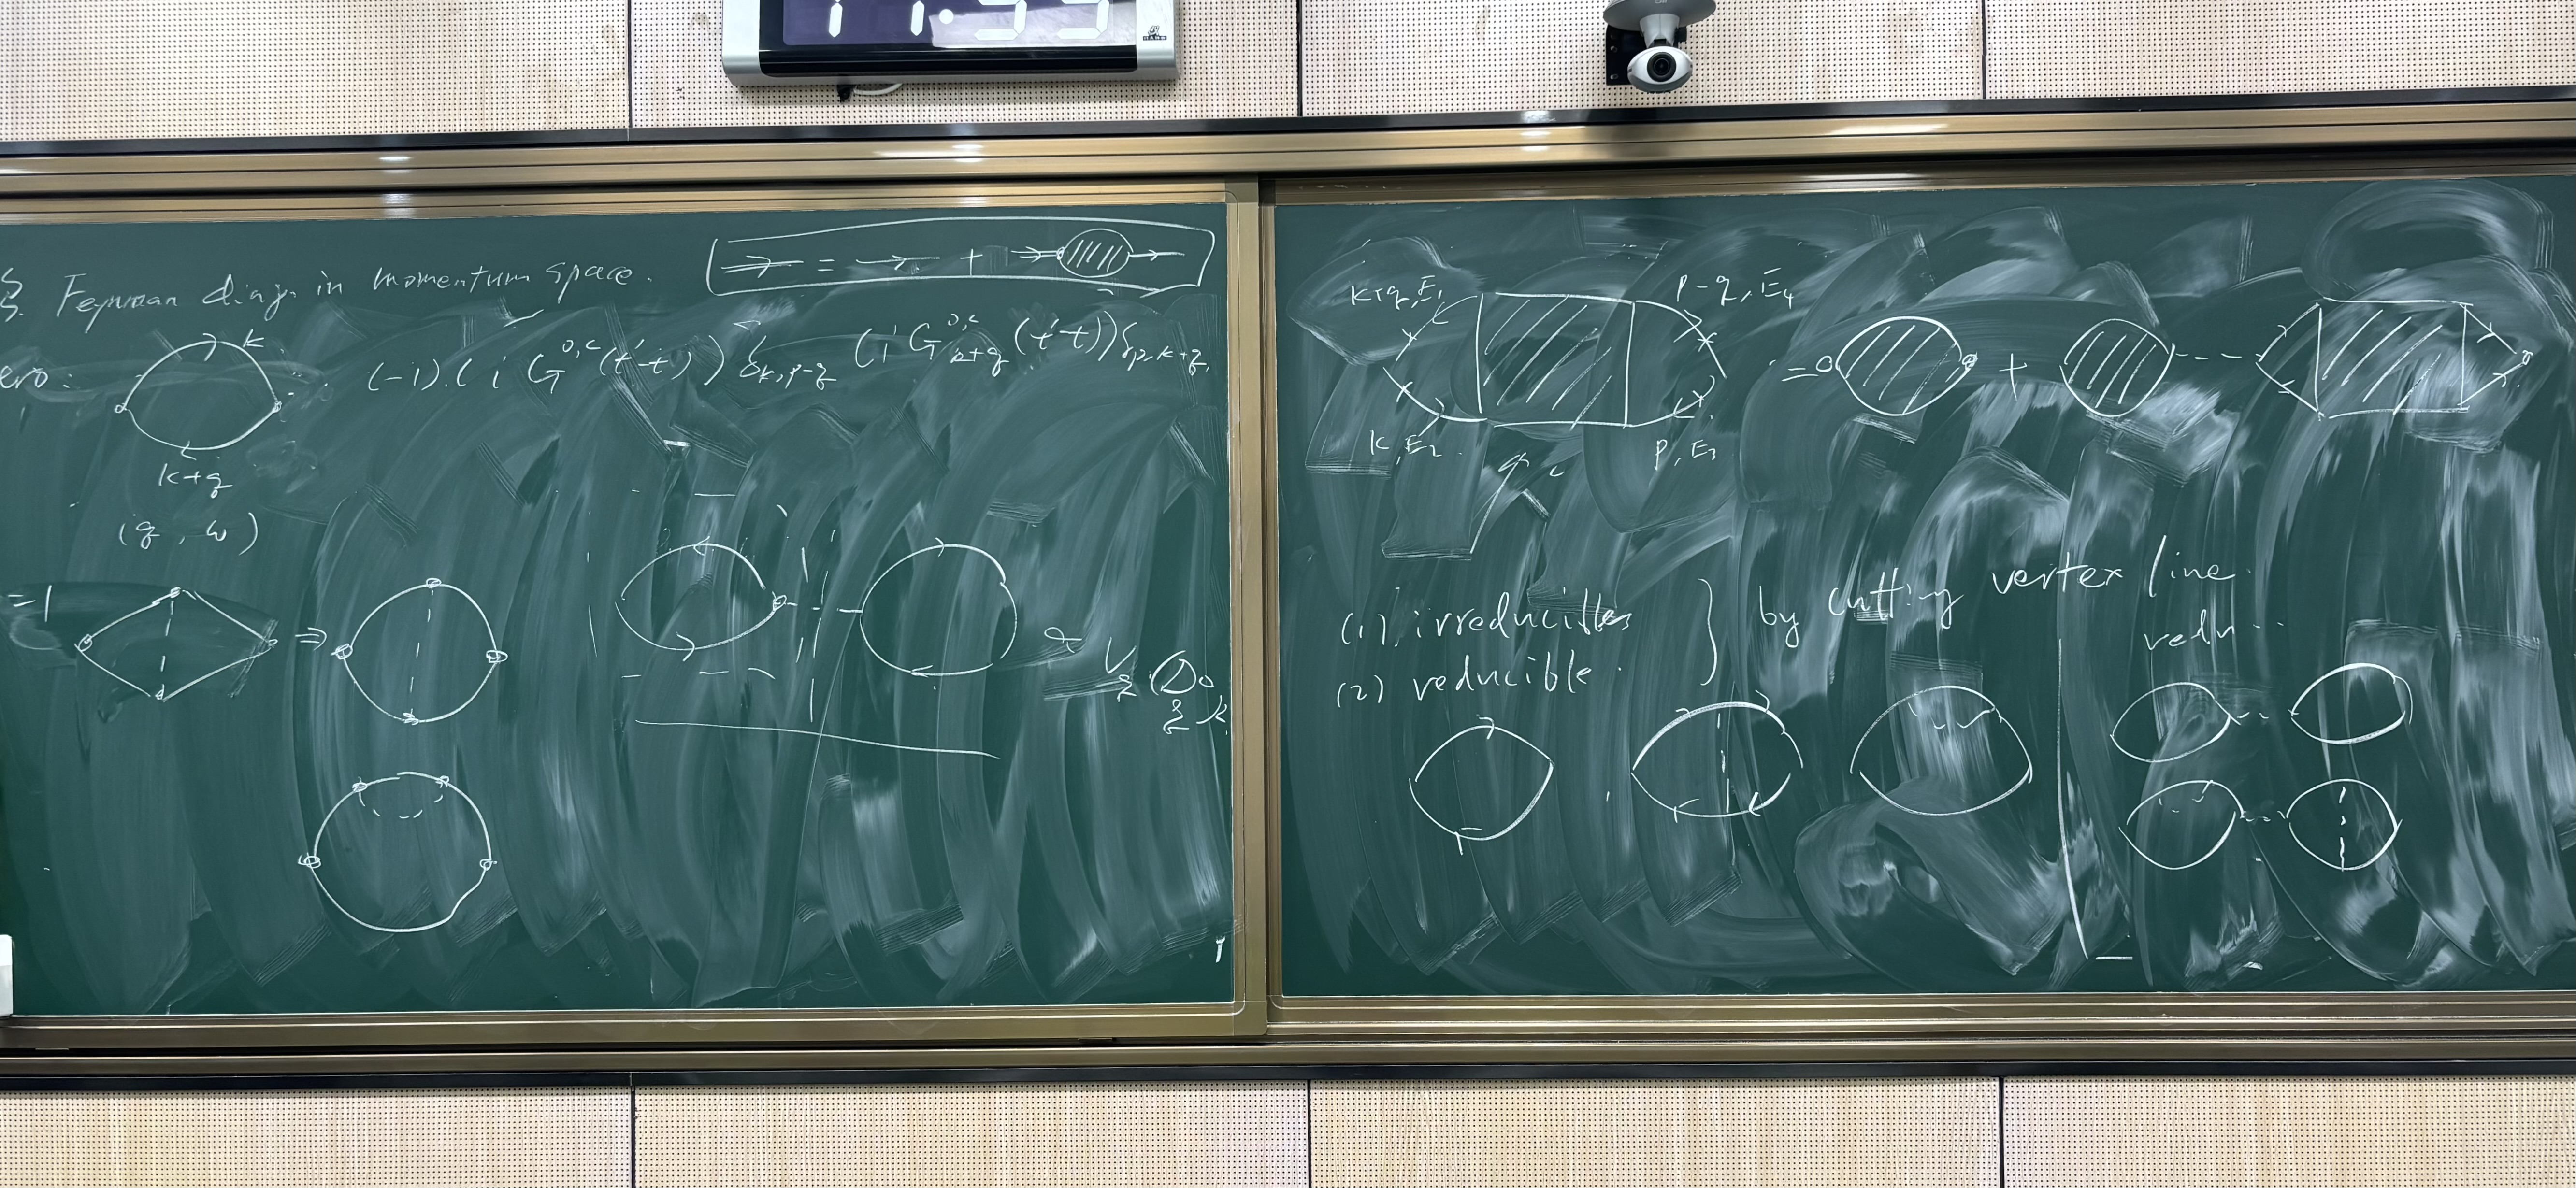
\includegraphics[width = \linewidth]{./media/feynmann20.jpeg}
\end{center}
\[
  D_q(E) = \frac{\Lambda_q(E)}{1 - \Lambda_q(E) V(q)}, \quad
  G = \frac{G^{0,c}}{1 - G^{0,c} \Sigma}
\]
Organizing principle, recursive structure.
\[
  U(t,t') = T_\epsilon \exp\ab(-\frac\iu\hbar \int \d t' H(t'))
\]
Vertex function/convention.
Skeleton diagram \texttt{<->}Schigon:
\[
  \iu\pdif t G = \delta + \braket<\Gamma c^\dagger c>.
\]
\begin{center}
  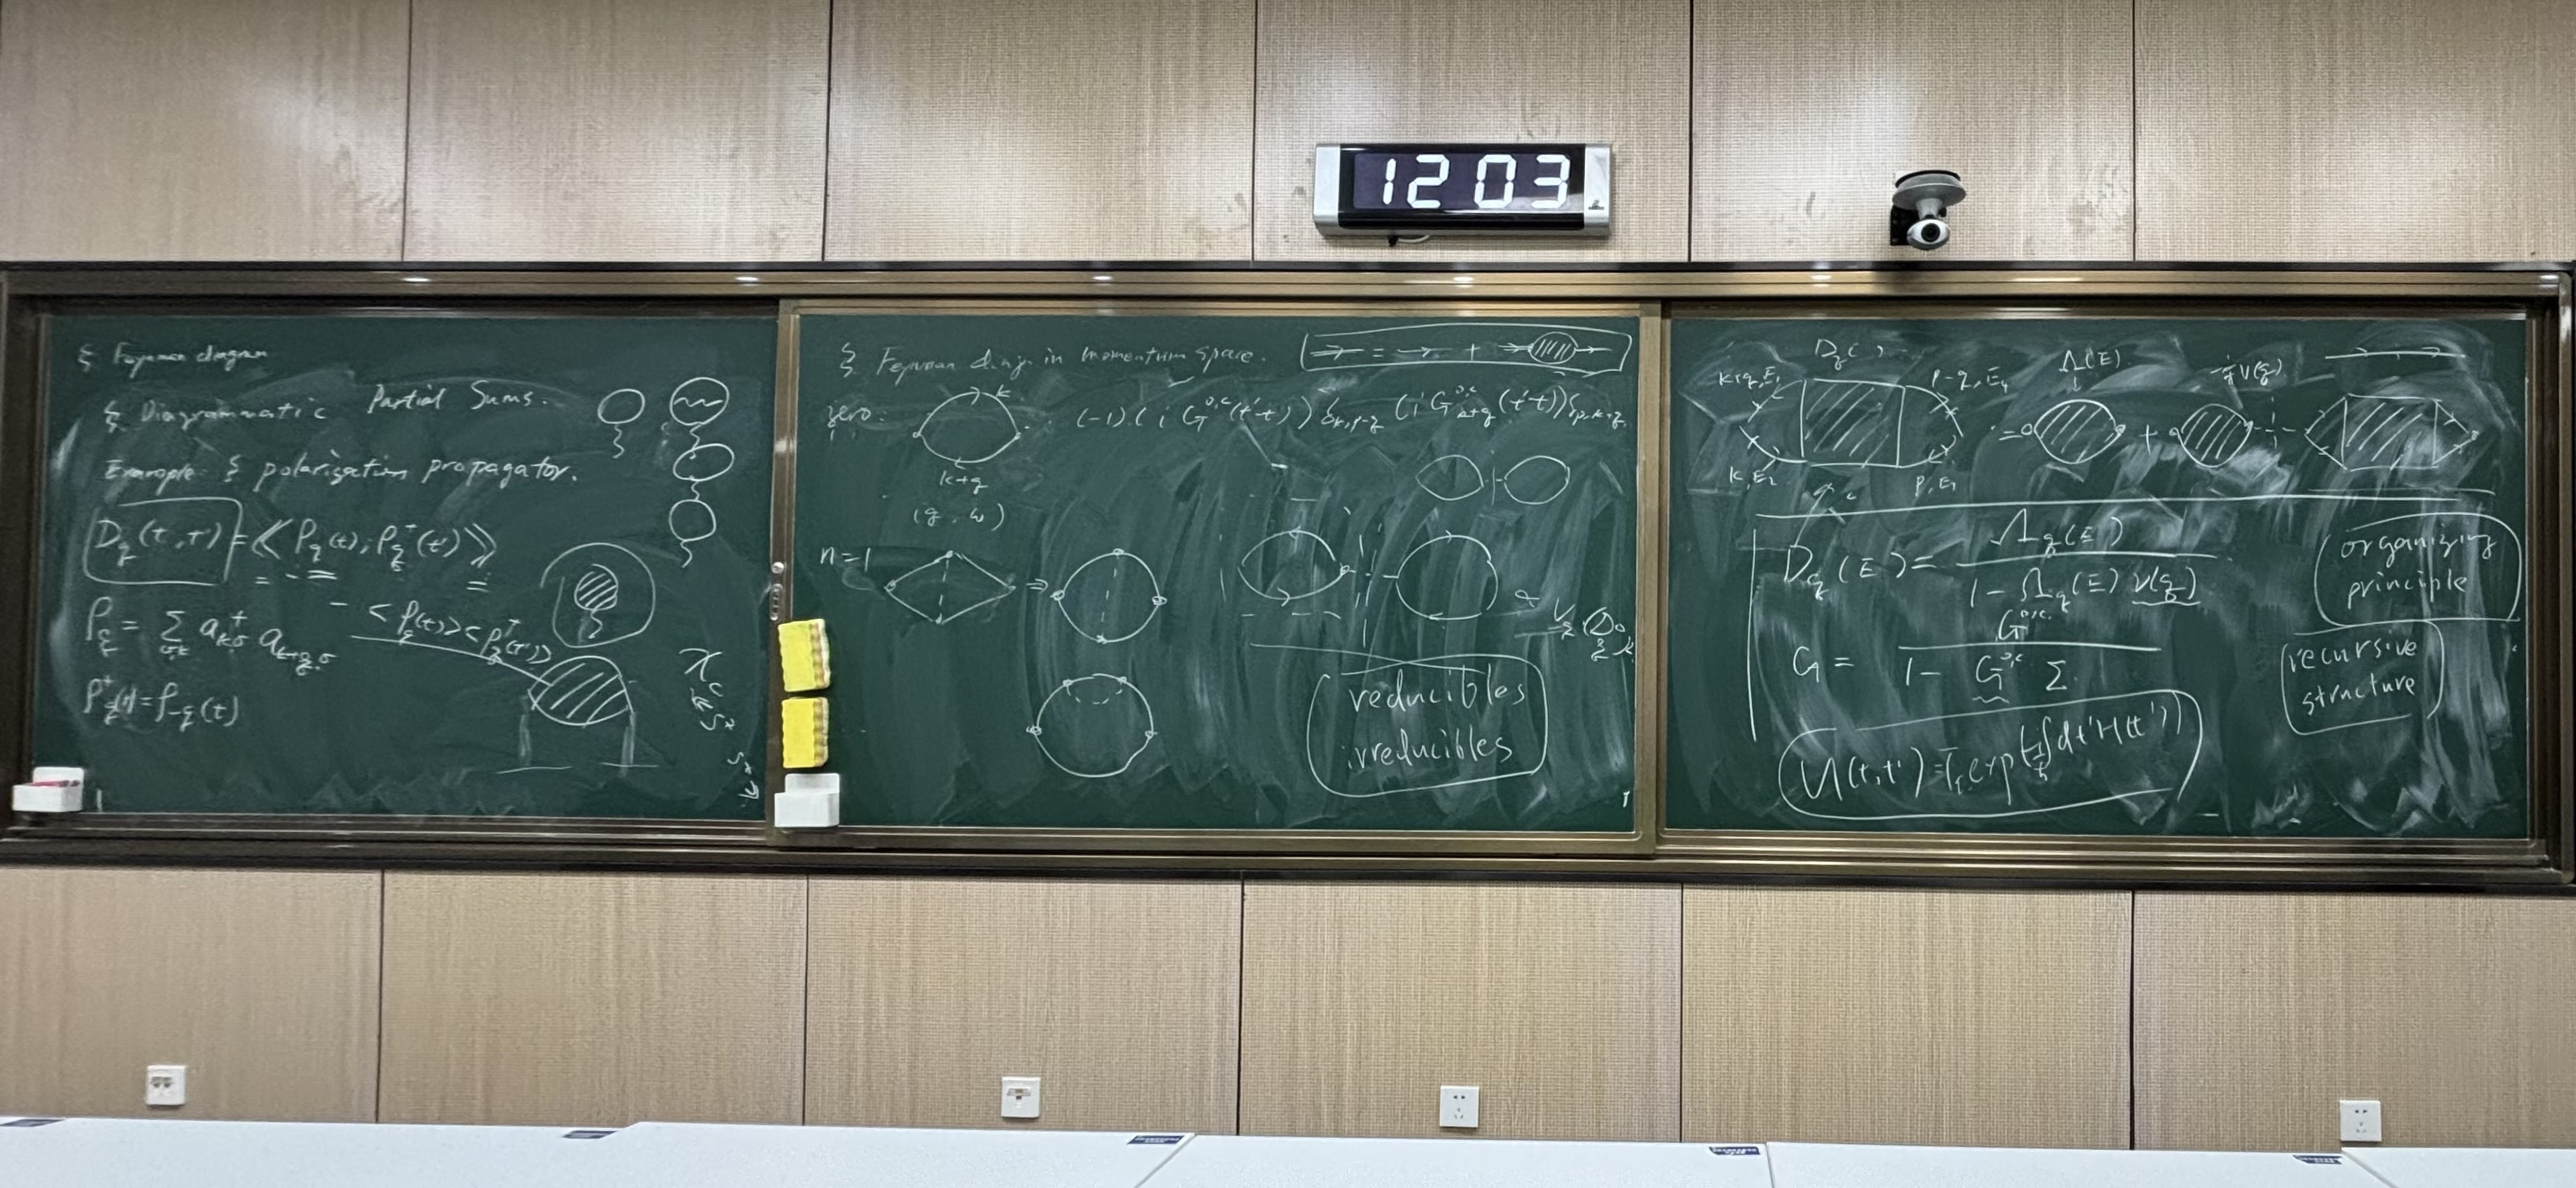
\includegraphics[width = \linewidth]{./media/feynmann21.jpeg}
\end{center}

\subsection{Partial resum}

For Green functione $G$
\[
\]
which gives us Dyson equation.
\[
  V_\text{eff}(q,E) = \frac{\nu(q)}{1 - \nu(q) \Omega_q(E)}
  \qq{Dielectric function}
\]
Trieste, Fabrizio 2022.
\begin{center}
  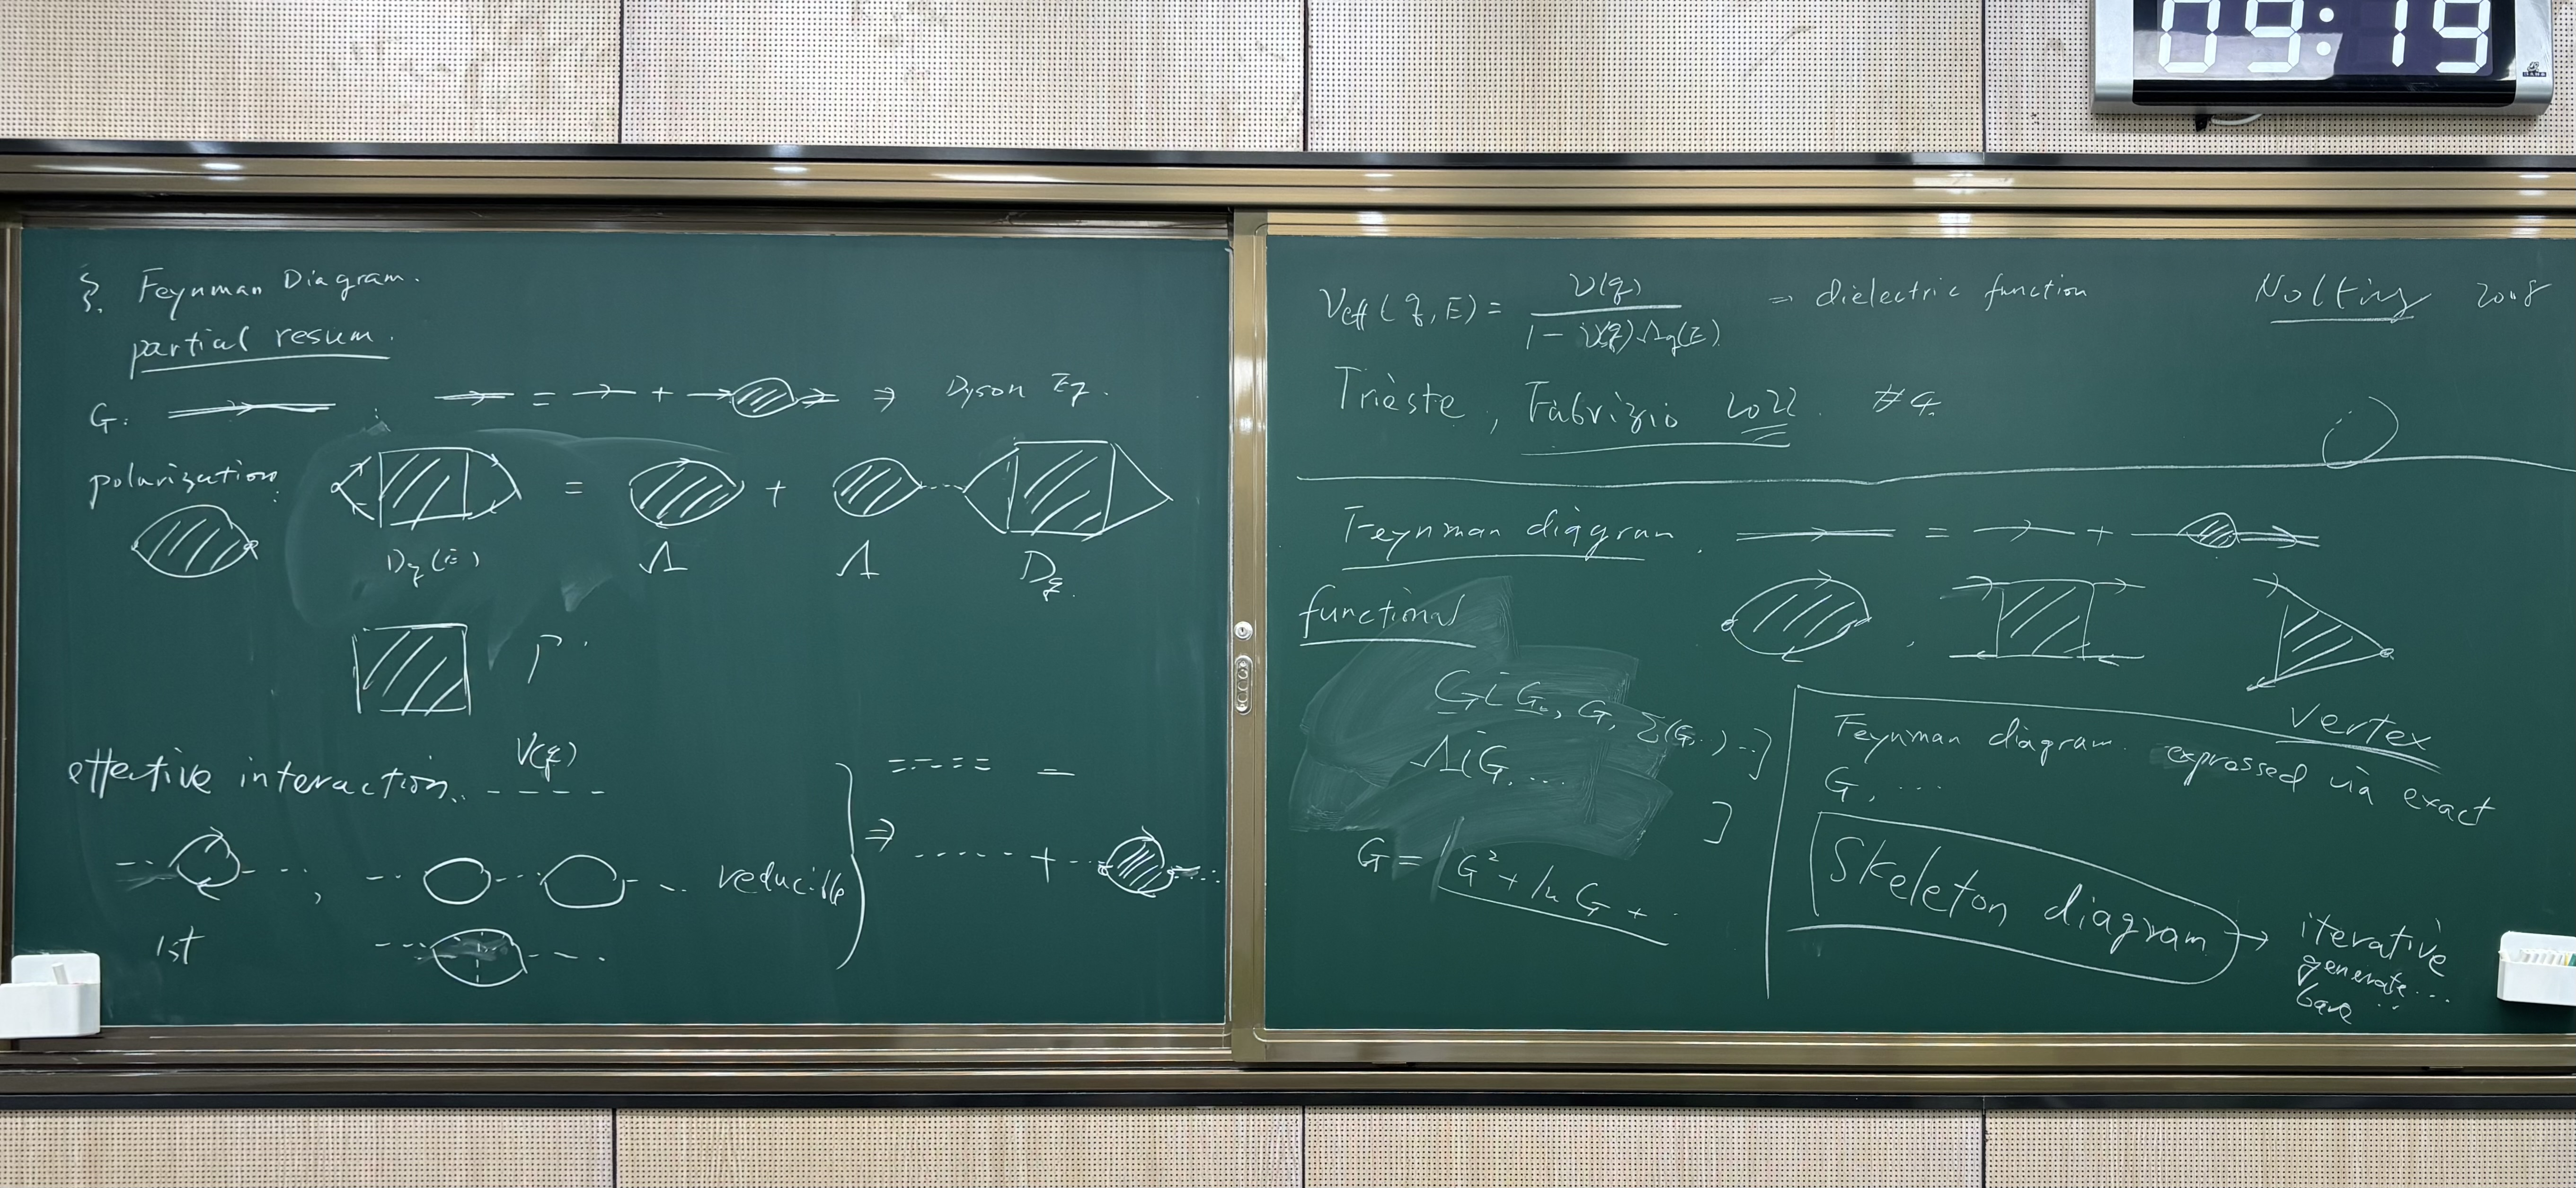
\includegraphics[width = \linewidth]{./media/feynmann22.jpeg}
\end{center}
The Feynman diagram can be expressed via exact $G$, etc. This is so-called the
Skeleton diagram. One can use it to iteratively generate bare sequences.
\paragraph{Skeleton diagram}
Structure of exact solution algebraic relation.

In QFT: scattering amplitudes recursive relations.
\begin{center}
  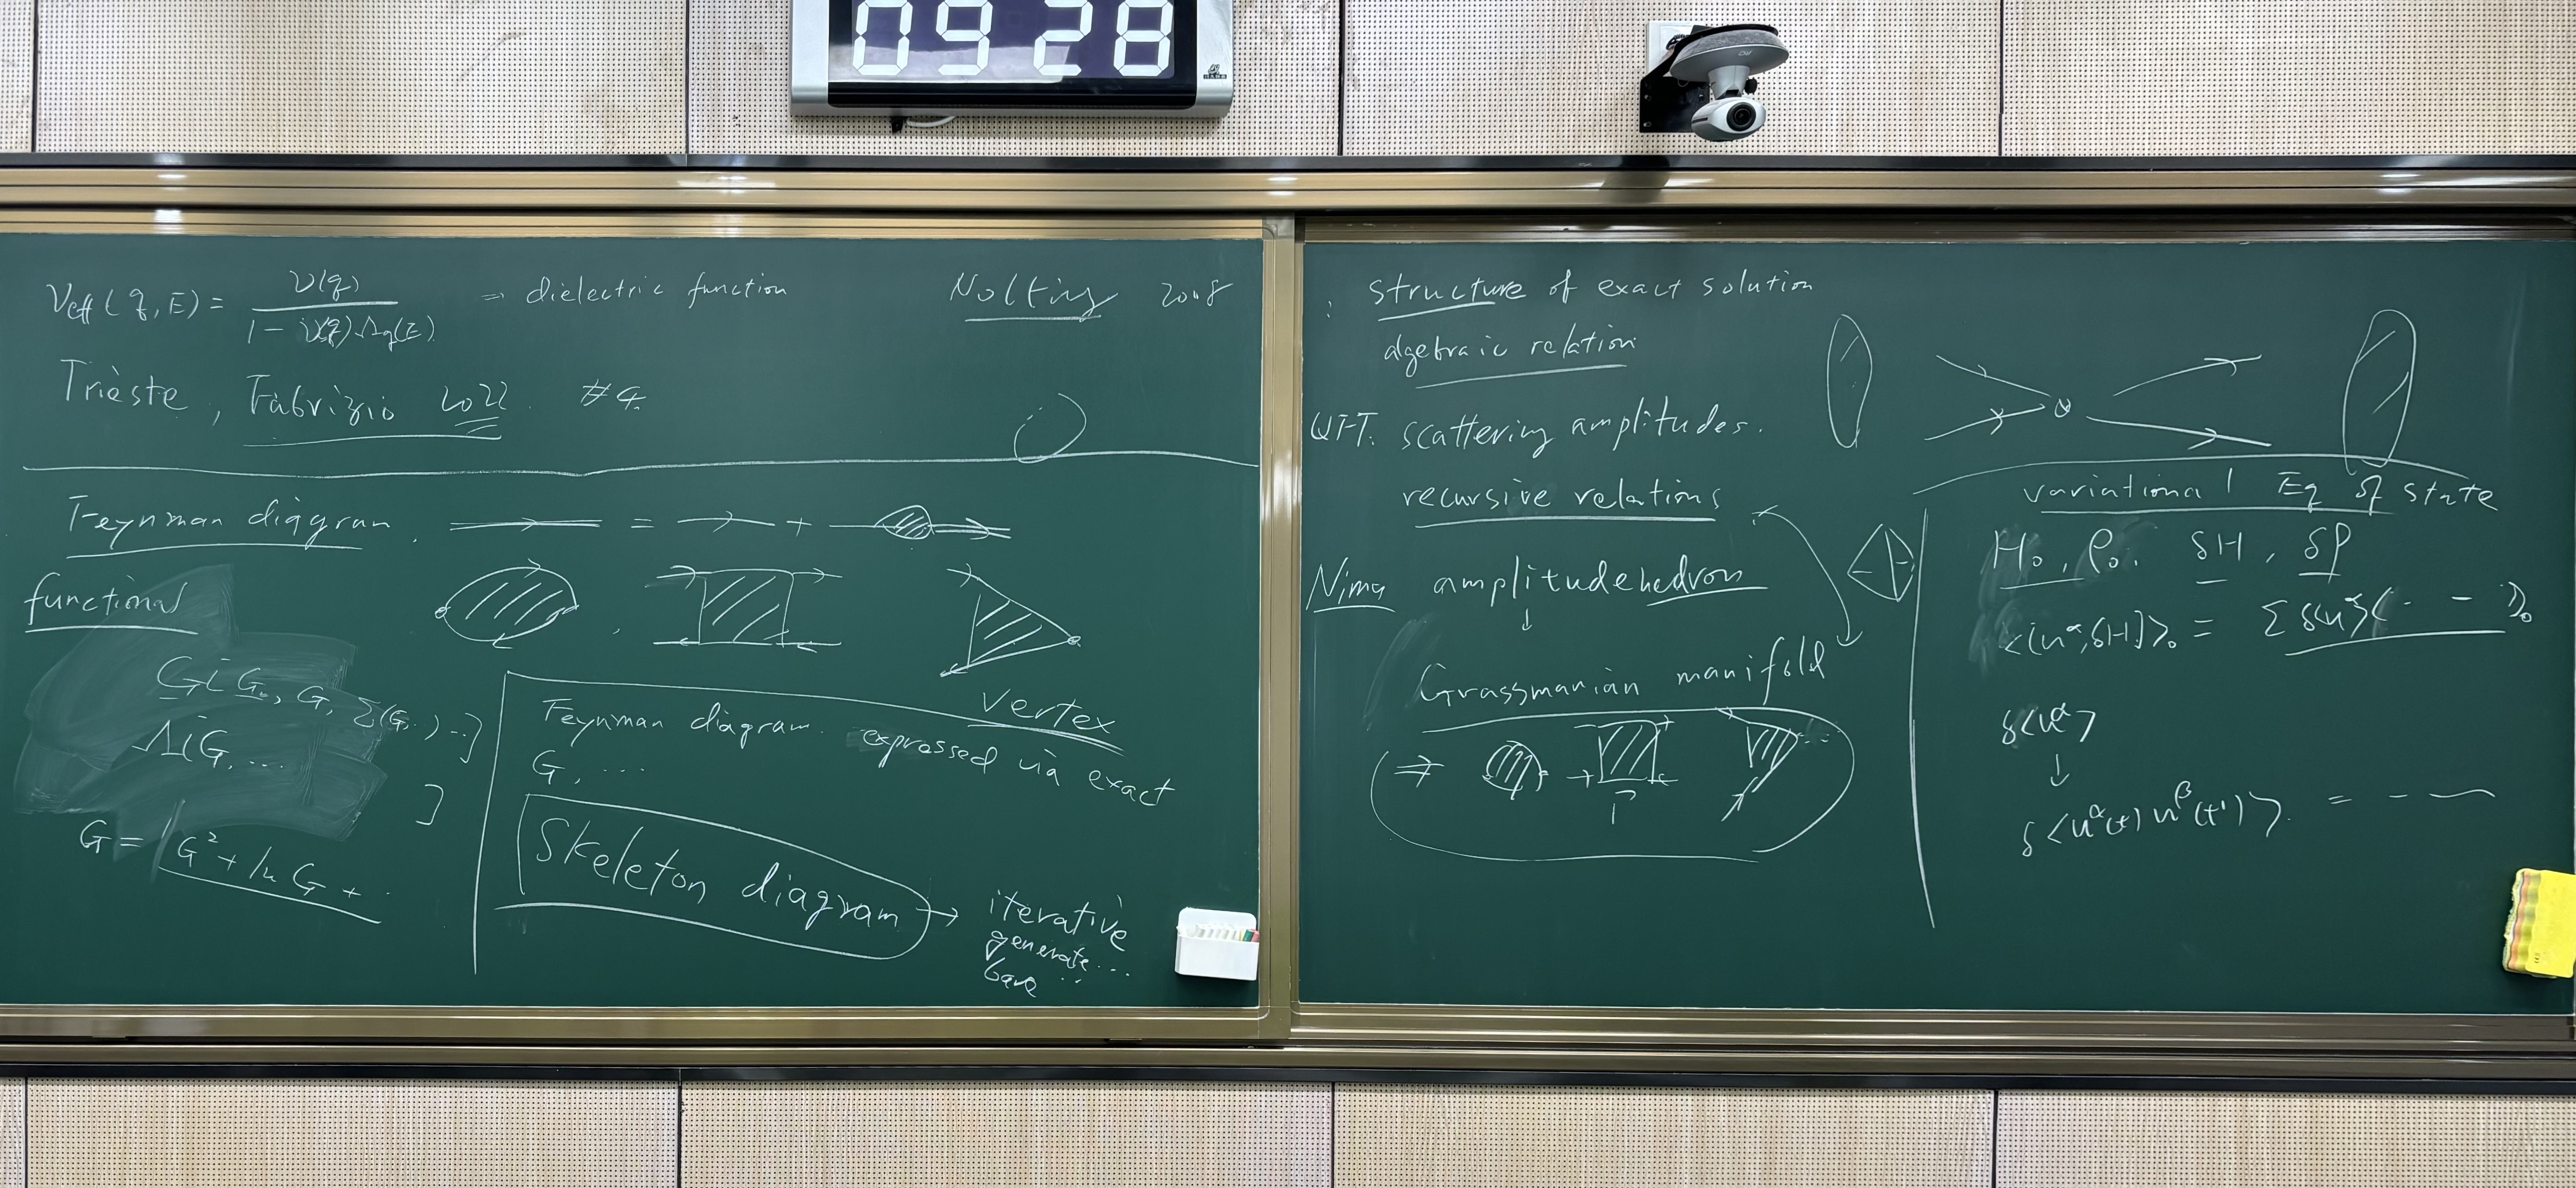
\includegraphics[width = \linewidth]{./media/feynmann23.jpeg}
\end{center}

\subsection{Two-particle Green's functions \& correlation functions}

\begin{multline*}
  K_{\sigma_1\sigma_2\sigma_3\sigma_4}(\tau_1p_1,\tau_2p_2;\tau_3p_3,\tau_4p_4)
= -\braket<\mathcal T_\tau(\wick{
  \c4 c_{p_1\sigma_1}(\c2\tau_1)
  \c1c_{p_2\sigma_2}(\c3\tau_2)
  \c1c_{p_3\sigma_3}^\dagger(\c4\tau_3)
  \c2 c_{p_4\sigma_4}^\dagger(\c3\tau_4)})>\\
  \xlongequal0 -\delta_{\sigma_1\sigma_4} \delta_{\sigma_2\sigma_3} G_{14}G_{23}
  + \delta_{\sigma_1\sigma_3} \delta_{\sigma_2\sigma_4} G_{13}G_{24}
\end{multline*}
The equation of motion becomes
\[
  \ab(\pdv*{}t - G_k)G_0(\tau', k) = \delta(\tau'), \quad
  \ab(\pdv*{}t - G_k)G = \delta(\tau')
- \frac1V \sum_{\bm p\bm q\alpha} U(\bm q)
  \braket<T_\tau(
    c_{p+q,\alpha}^\dagger(\tau') c_{p\alpha}(\tau')
    c_{k+q}(\tau') c_{k\sigma}^\dagger
  )>
\]
where $\delta H = \frac1{2V} \sum_{\substack{kpq\\\alpha\beta}} u(q)
  c_{p_1\alpha}^\dagger c_{k+q,\beta}^\dagger c_{k\beta} c_{k+q,\alpha}$.
Integrate over the EOM
\begin{multline*}
  \int \d\tau' G_0(\tau - \tau', k)
    \ab(-\pdv*{}{\tau'} - \epsilon_k) G(\tau', k)\\
= G_0(\tau, k) - \frac1V \sum u(q) \int \d\tau' G_0(\tau - \tau',k)
  k_{0\alpha;\alpha\sigma}(\tau'k+q, \tau'p;\tau' + 0^+, p+q, 0k)
\end{multline*}
where $k$ can be expressed in diagram
\begin{center}
  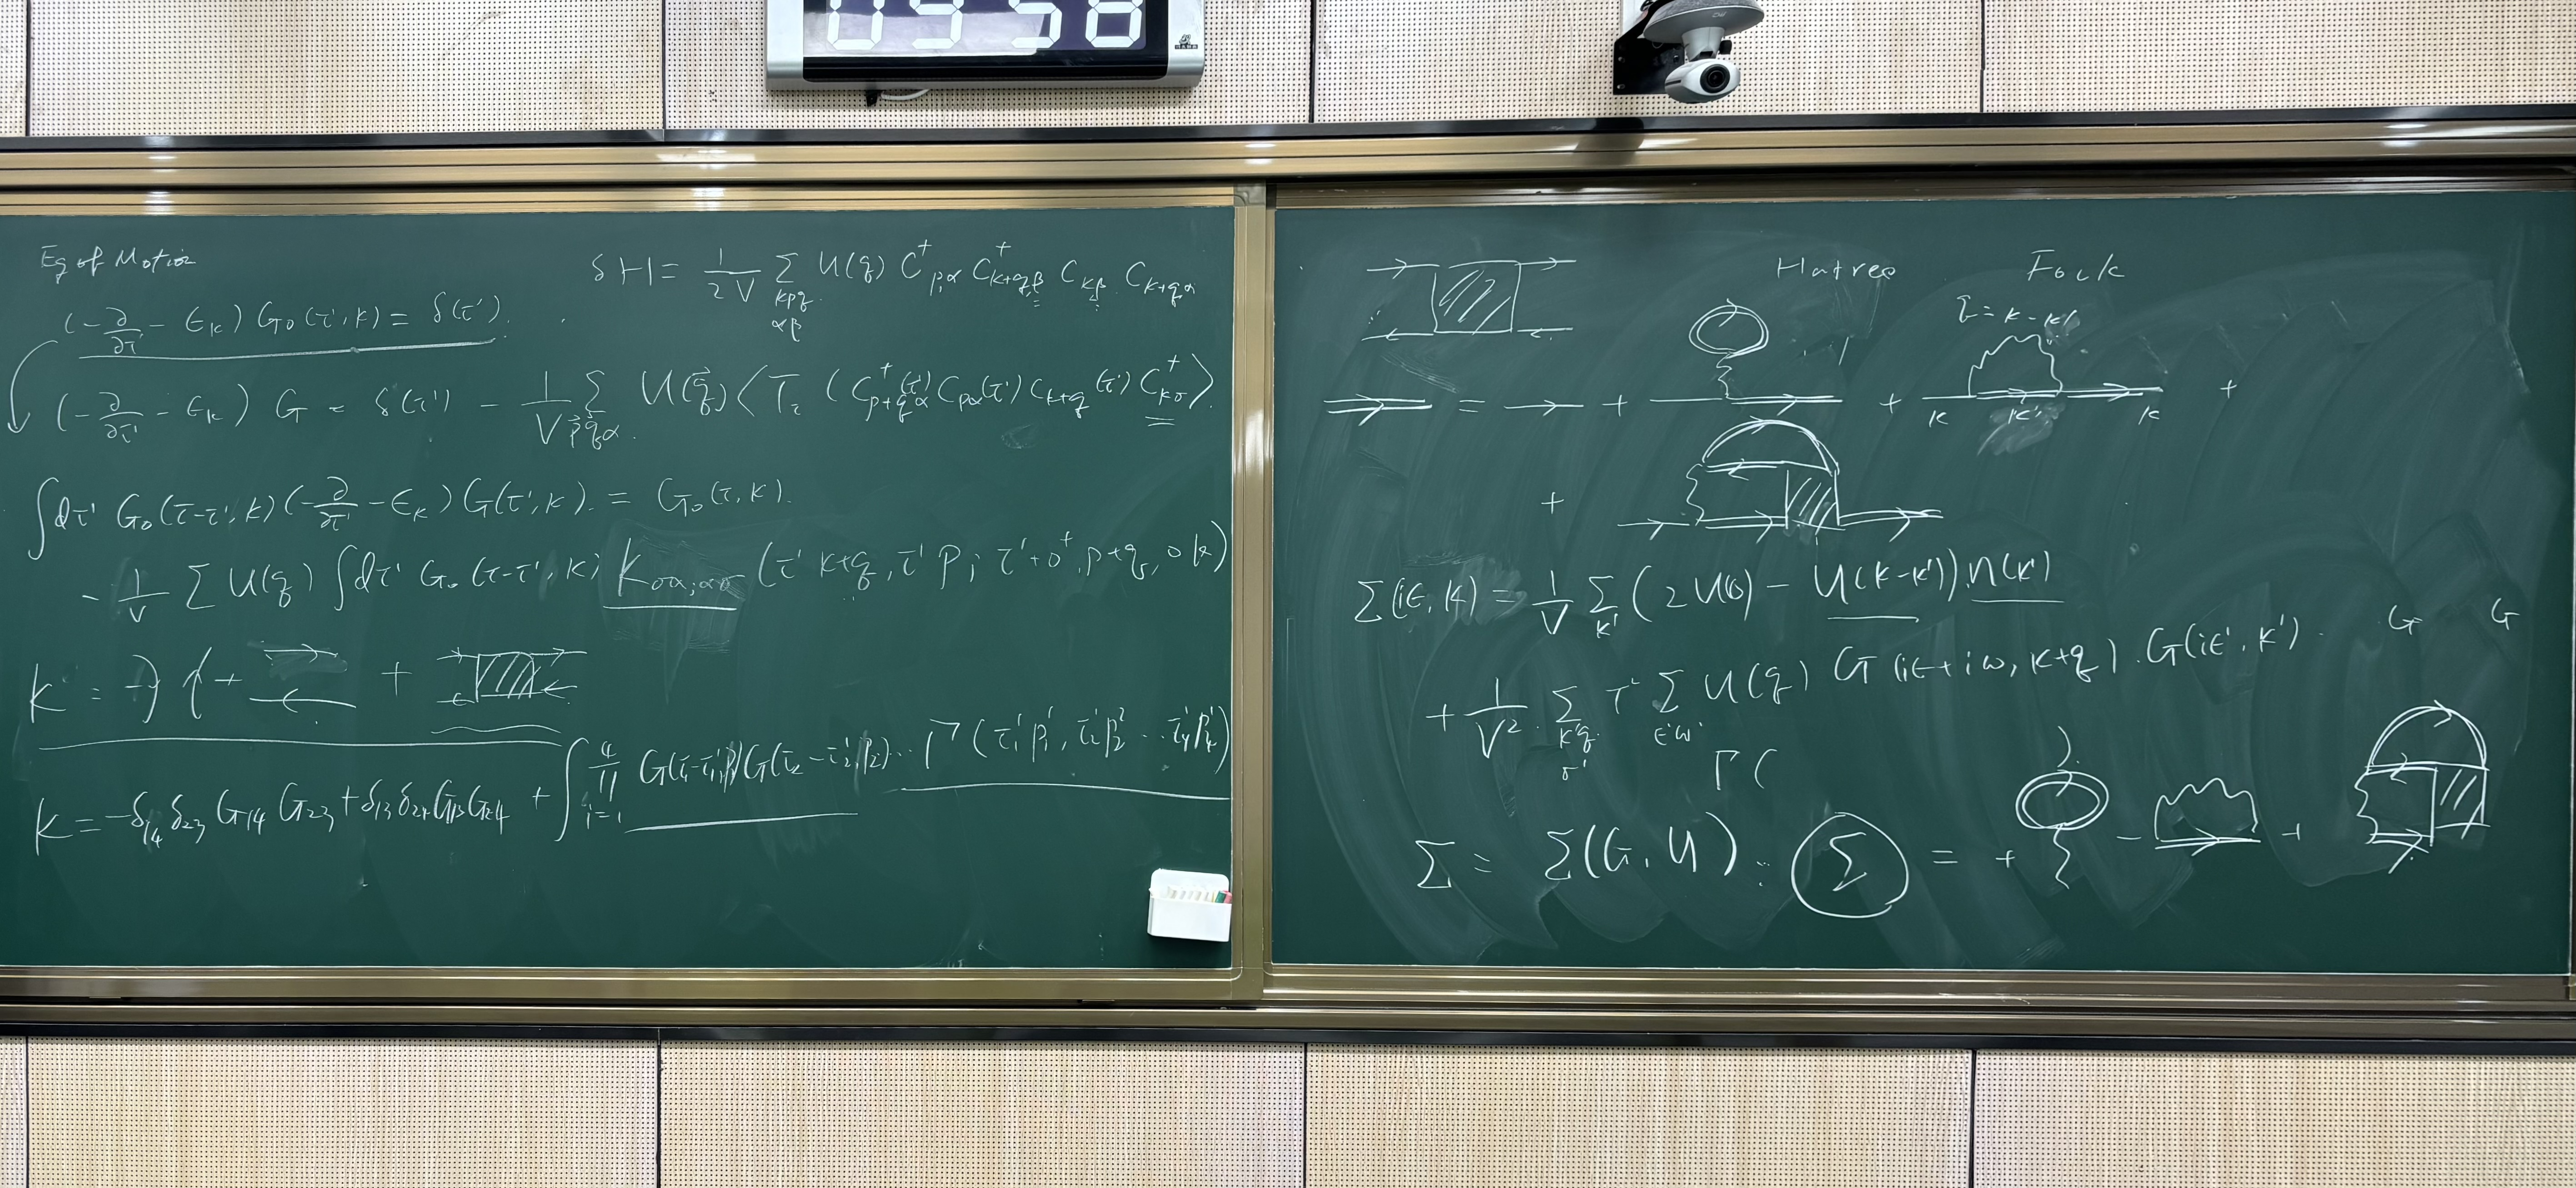
\includegraphics[width = \linewidth]{./media/feynmann24.jpeg}
\end{center}
or equation
\begin{multline*}
  k = -\delta_{14} \delta_{23} G_{14} G_{23}
    + \delta_{13}\delta_{24} G_{13}G_{24}
    + \int \prod_{i=1}^4 G(\tau_1 - \tau_1', p_1) G(\tau_2 - \tau_2', p_2)
      \cdots \\
      \Gamma(\tau_1' p_1', \tau_2'p_2^2,\cdots\tau_4'p_4')
\end{multline*}
The self energy
\[
  \Sigma(\iu\epsilon, k) = \frac1V \sum_{k'}(2U(0) - U(k - k'))U(k')
+ \frac1{V^2} \sum_{kq\sigma'} \tau^2 \sum_{\epsilon'\omega'} U(q)
  G(\iu\epsilon + \iu\omega, k + q) G(\iu\epsilon', k)
  \quad G \quad G \Gamma(\quad)
\]
can see that $\Sigma$ is a functional of $\Sigma(G, U)$, which can be
represented by Feynman diagram.

\subsection{Correlation functions}

Momentum density operators
\begin{align}
  A(q) & = \sum \Lambda_0^A (k\alpha,k + q \beta)
           c_{k,\alpha}^\dagger c_{k+q,\beta},\\
  B(q) & = \sum_k \Lambda_0^B (k,\alpha; k + q, \beta)
            c_{k\alpha}^\dagger c_{k+q,\beta}
\end{align}
We define the conductivity
\[
  \sigma:\ \bm E \to \braket<\bm j>,
\]
and define the current operator
\[
  \nabla \cdot {\bm j} = [\rho_n, H_0], \quad
  j_x = \sum_{q, k} \pdif{k_x} \epsilon(\bm k) c_{k+q_x}^\dagger c_{\bm k}
\]
by the momentum along the $x$-direction.
\begin{multline*}
  \chi_{AB}(\tau, q) = -\frac1V \braket<T_\tau A(q,\tau) B(-q, 0)>
= \frac1V \sum \Lambda_0^A \Lambda_0^B K
= -\frac{\delta_{q,0}}{V} \braket<A(0)B(0)>\\ + \frac1V \sum_{k+\beta}
    \Lambda_0^A \Lambda_q^B G(\tau, k + q) G(-\tau, k)
  + \frac1V \sum \Lambda_v^A \Lambda_0^B
  \int \prod{i=1}z_{i=1}^q \d\tau_i G \cdots G\Gamma(\quad)
\end{multline*}
\begin{center}
  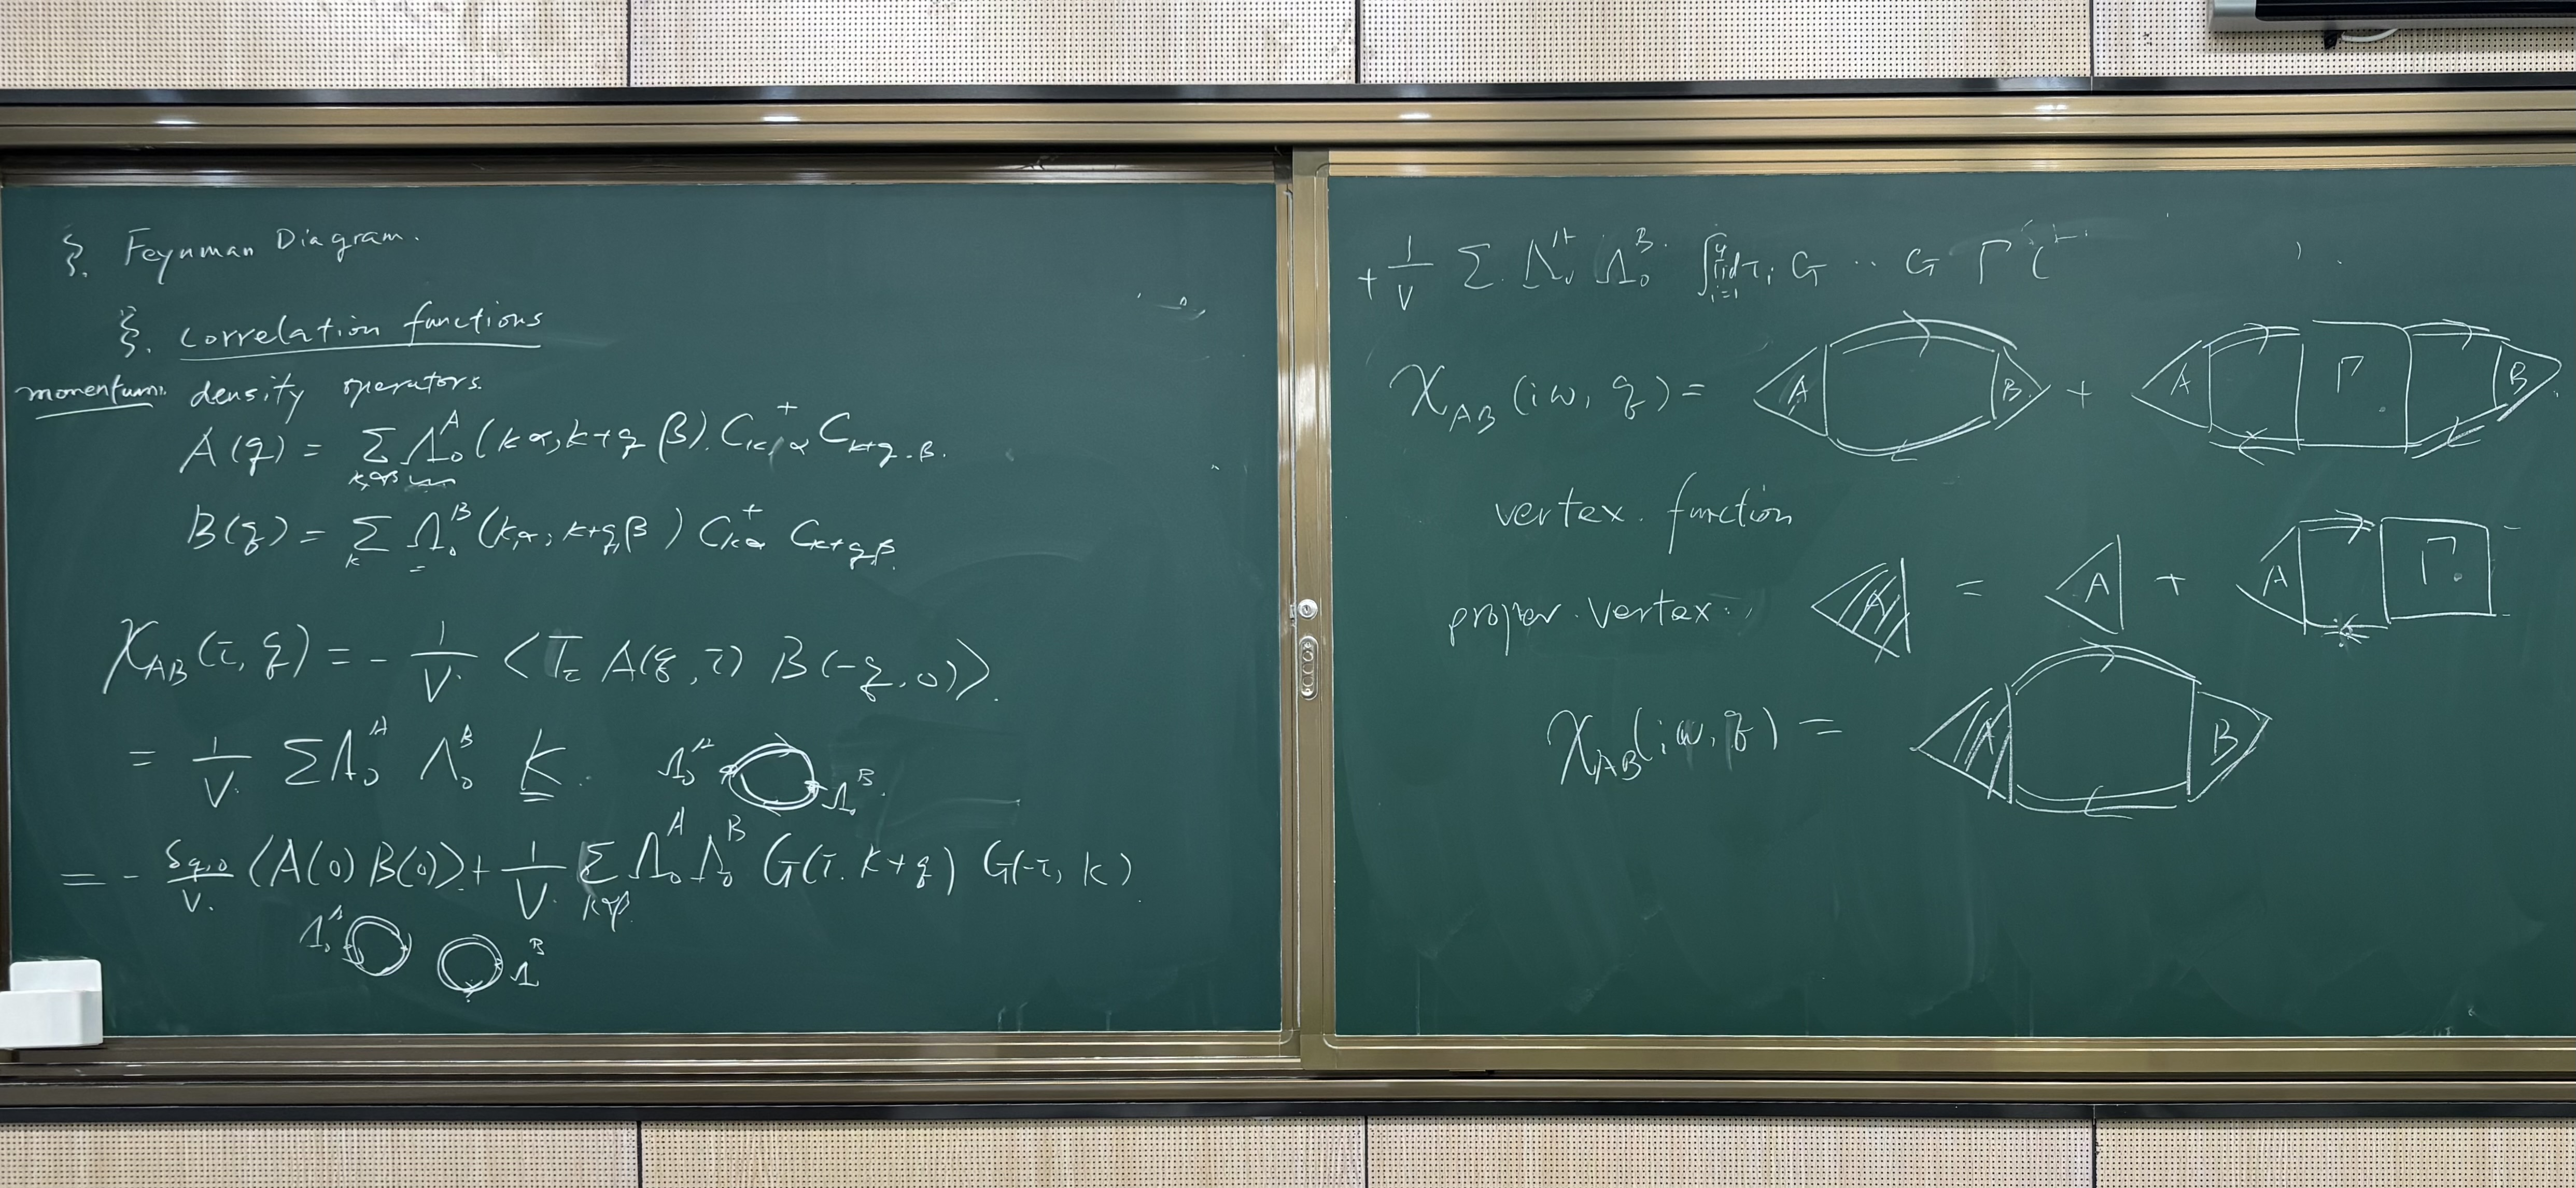
\includegraphics[width = \linewidth]{./media/feynmann25.jpeg}
\end{center}
From $\bm E = 0^+$
\[
  \bm\sigma = \fdv*{\braket<\bm j>}{\bm E}
= \fdv*{\braket<\sum_q \Lambda_0^A(c^\dagger c)>}{\bm E}
= \fdv*{\sum_q \Lambda_0^n G[k + q, \cdots, ]G,\Sigma}{\bm E}
= \Lambda_0 G \fdv*{\quad}E \to \Gamma
\]
Then, the electric field can be cuopled to the charge
density $\bm E (\propto \mu: -\nabla\mu) \cdot e\hat n$.
$\Lambda$ can be expressed as $1$ and vertex.
\begin{center}
  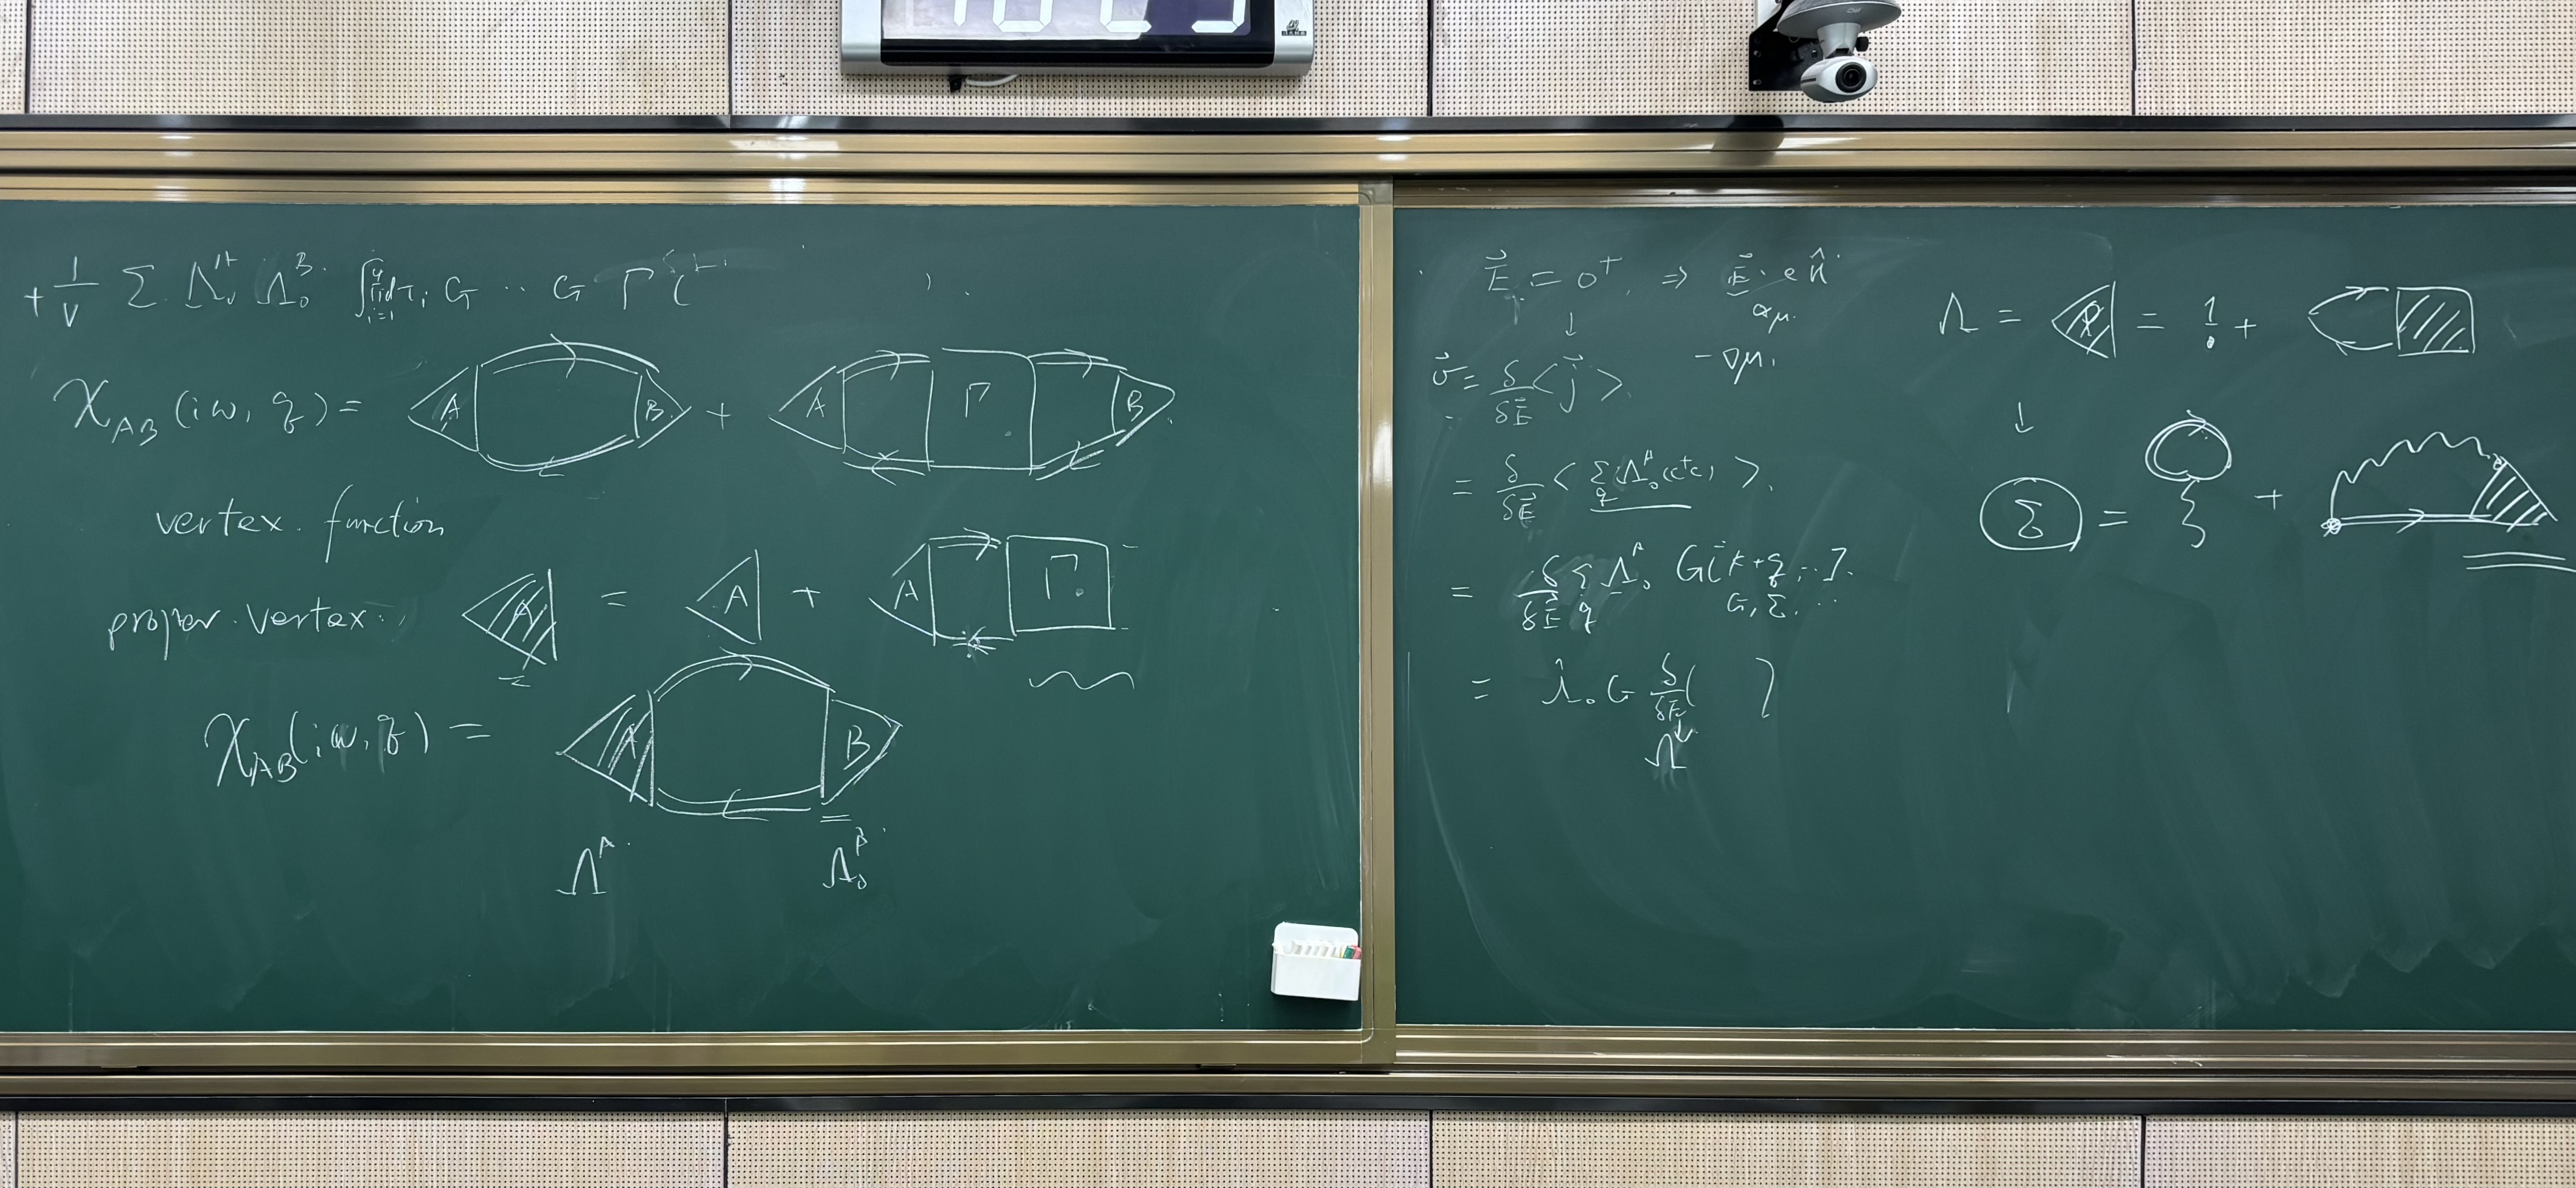
\includegraphics[width = \linewidth]{./media/feynmann26.jpeg}
\end{center}

\subsection{Scwhinger's approach (variational / quantum action)}

\[
  \iu \pdif t G = \delta(t) + \braket<[H, C]^{(+)}; c^\dagger>
= \delta(t) + \sum_{pq\alpha}
  \braket<T_\tau(c_{p+q}^\dagger(t) c_p(t) c_{k+q}(t;c_{k\sigma}^\dagger))>
\]
where $\Lambda$ can be defined from functional derivative
\[
  \Lambda:\ \braket<\hat n_p c_k(t); c_k^\dagger(0)>
= \fdv*{G^*(\quad;\nu_{n_p})}{\nu_{n_p}}\bigg|_{\nu\to 0}
\]
Adding to the original Hamiltonian
\[
  H^* = H_0 + \nu_{np} \hat n_p, \qq{Source field.}
\]
The Green function
\[
  \hat G = \frac1{\omega\identity - H}, \quad \hat G\hat G^{-1} = \identity
\]
So, the functional derivative
\[
  \fdv*{[\hat G\hat G^{-1}]}\nu = 0
= \fdv G\nu \hat G^{-1} + \hat G\fdv{\hat G^{-1}}\nu
\]
from which we get
\[
  \fdv*G\nu
= -\hat G\underset{\text{vertex function}}{\ab(\fdv*{\hat G^{-1}}\nu)} G
\]
Denote $\Lambda = -\fdv*{G^{-1}}\nu$
\[
  \iu\pdif t G = \delta(t) - G\Lambda G
\]
Then,
\[
  \underline{\iu \pdif t} G
= \delta(t) + \braket<[H_0 + \delta H, c](t); c^\dagger>
= \underset{\sim G_0^{-1}}{\underline{\delta(t) + \braket<[H, c]; c^\dagger>}} + u\fdv*G\nu
\]
From where we get
\[
  \iu \pdif t G_0 = \delta(t) + \epsilon_k \epsilon_0 \Rightarrow
  G_0 = \delta(t)(i\pdif t - \epsilon)^{-1}
  \Rightarrow \frac1{\omega - \epsilon_k}
\]
The inverse of $G_0$
\[
  G_0^{-1} = \omega - \epsilon_k \to \iu\pdif t - \epsilon_k
\]
satisfies
\[
  \omega\pdif tG = G_0^{-1} + UG\underset{\Lambda}{\ab(-\fdv*{G^{-1}}\nu)}G,
  \quad (\omega\pdif t - UG\Lambda) G = G_0^{-1}
\]
Then,
\[
  -\nu_{n_p} + G_0^{-1} - UG\Lambda = G^{-1}, \quad
  G^{-1} = G_0^{-1} - \nu - \Sigma, \quad \Sigma = UG + UG\Lambda.
\]
The first, second order functional derivative
\[
  -\fdv{G^{-1}}\nu = \Lambda \Rightarrow \Lambda
= 1 + UG\Lambda G - U(G\Lambda G)\Lambda - UG\ab(\fdv\Lambda\nu)
\]
\begin{center}
  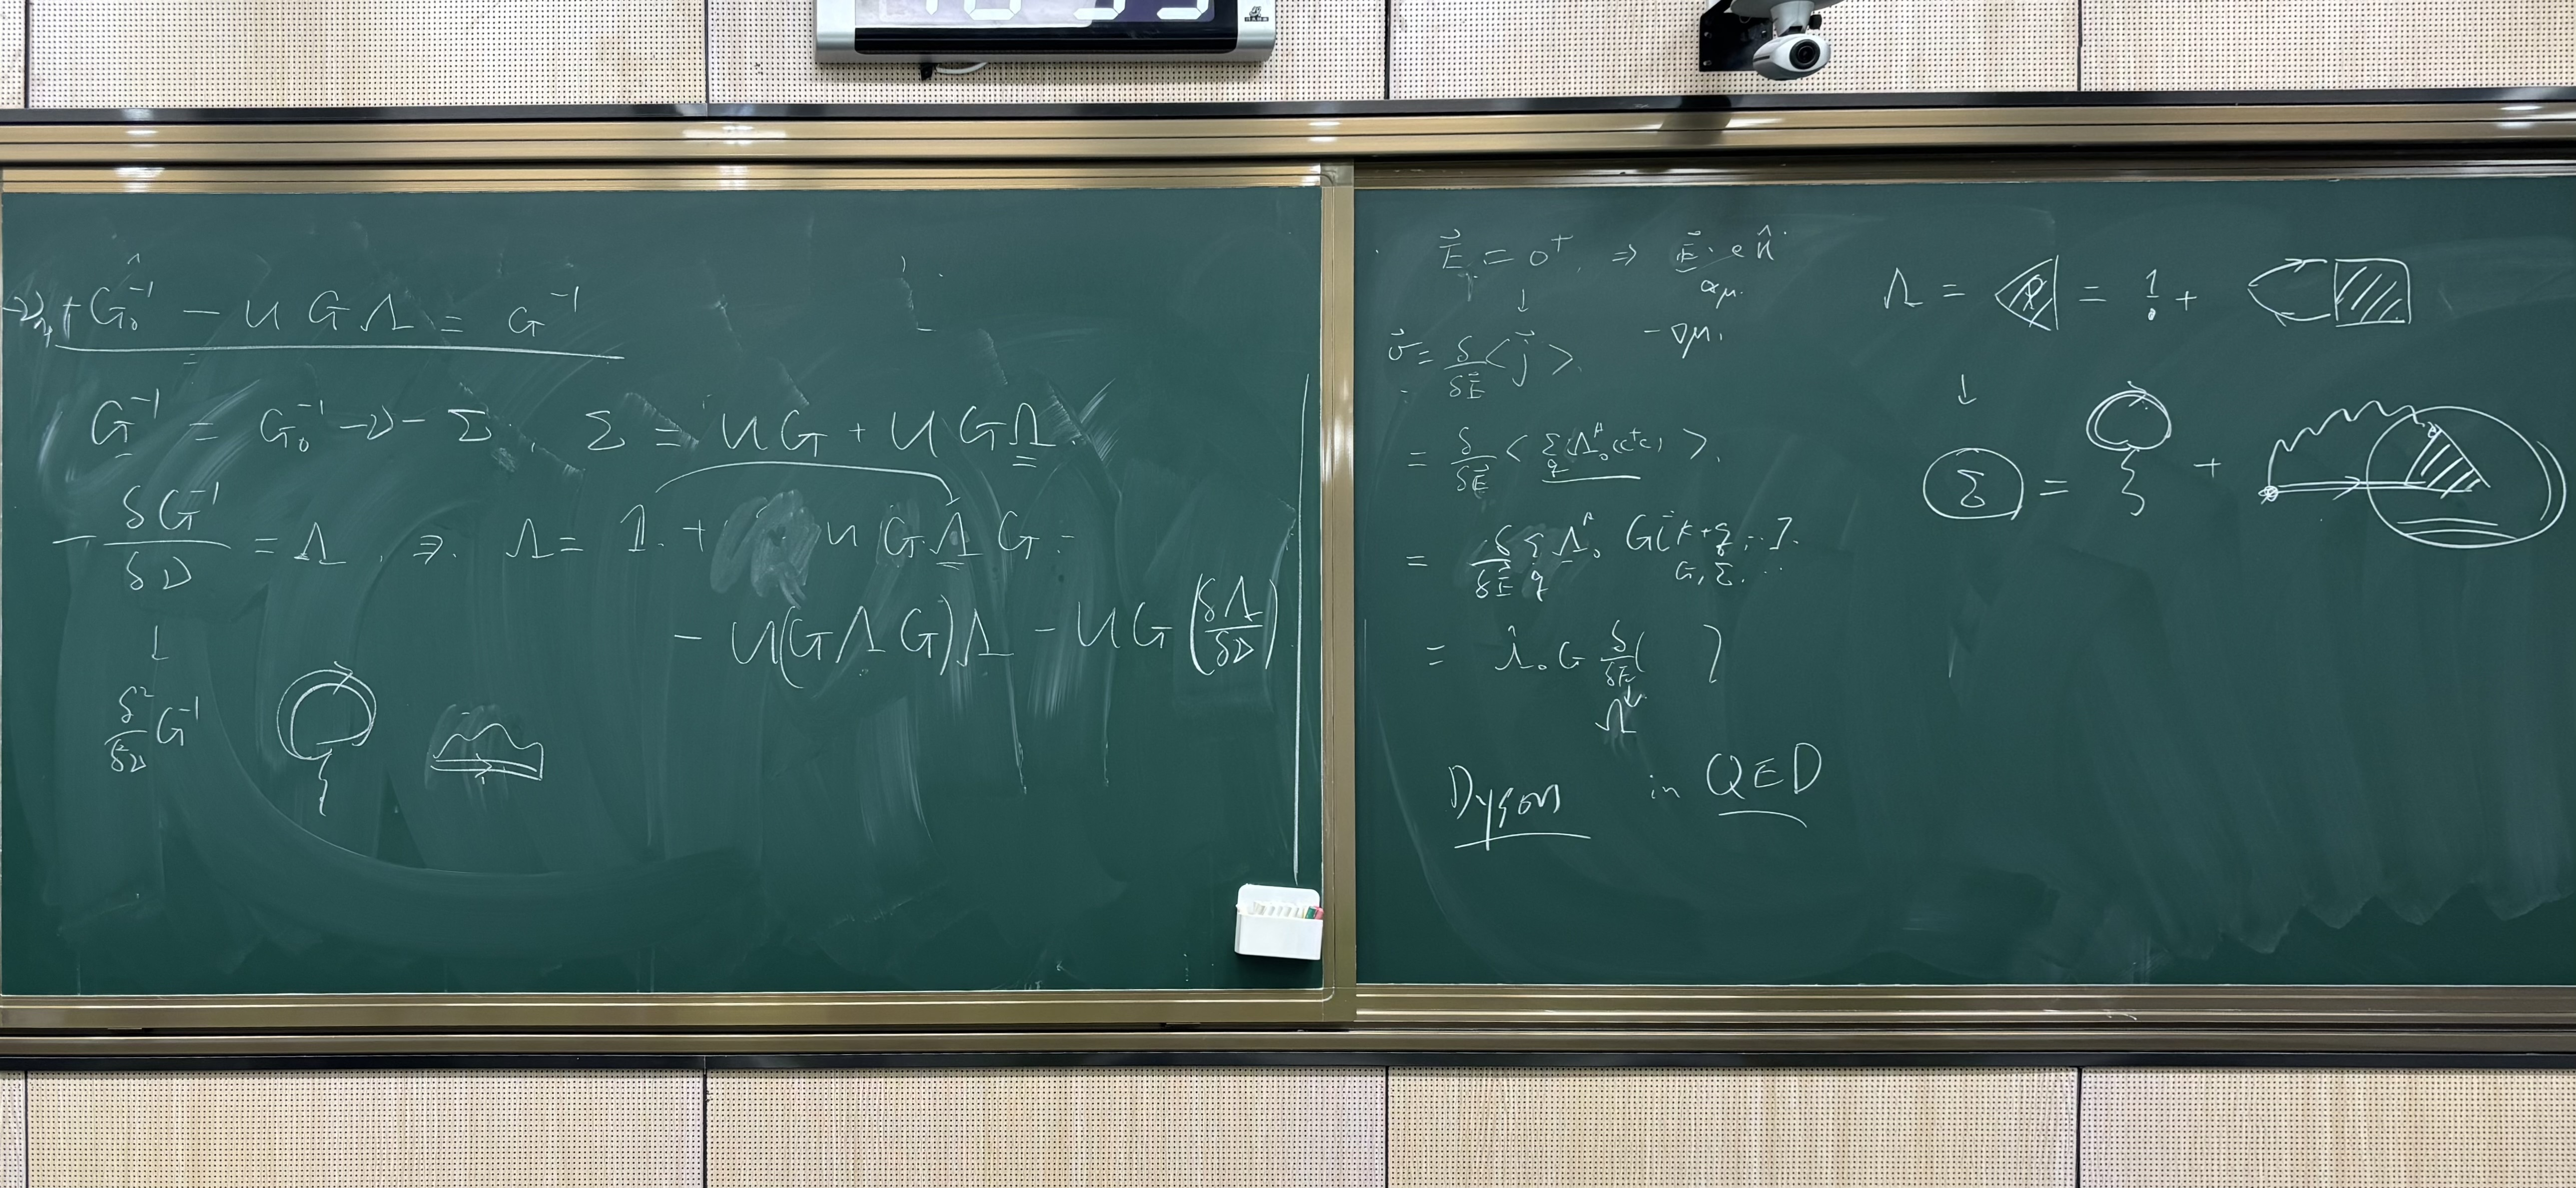
\includegraphics[width = \linewidth]{./media/feynmann27.jpeg}
\end{center}
\begin{multline*}
  G[c,c^\dagger] \to \braket<c(t), c^\dagger> \to \qq{Skeleton diagram}
  -\fdv*{G^{-1}}\nu \to \text{$\nu$ Dyson equation}, \\
  G^{-1} = G_0^{-1} - \nu - (UG + UG\Lambda)
\end{multline*}
The functional derivative
\[
  -\fdv*{G^{-1}}\nu = \identity + U\ab(-\fdv*G\nu) + U(-\fdv*[fun]{G\Lambda}\nu)
  \to U\ab[\ab(\fdv*G\nu)\Lambda - G\ab(\fdv*\Lambda\nu)]
\]
where $\fdv G\nu = -G\ab(\fdv*{G^{-1}}\nu) G$.
For the second order functional derivative, expanding the part
\[
  \fdv*{\fdv*{G^{-1}}{\nu(t_2)}}{\nu(t_1)} \to
  G\fdv*{}\nu \ab(\fdv*{G^{-1}}\nu)
\]
gives the diagram on the south west block.
\begin{center}
  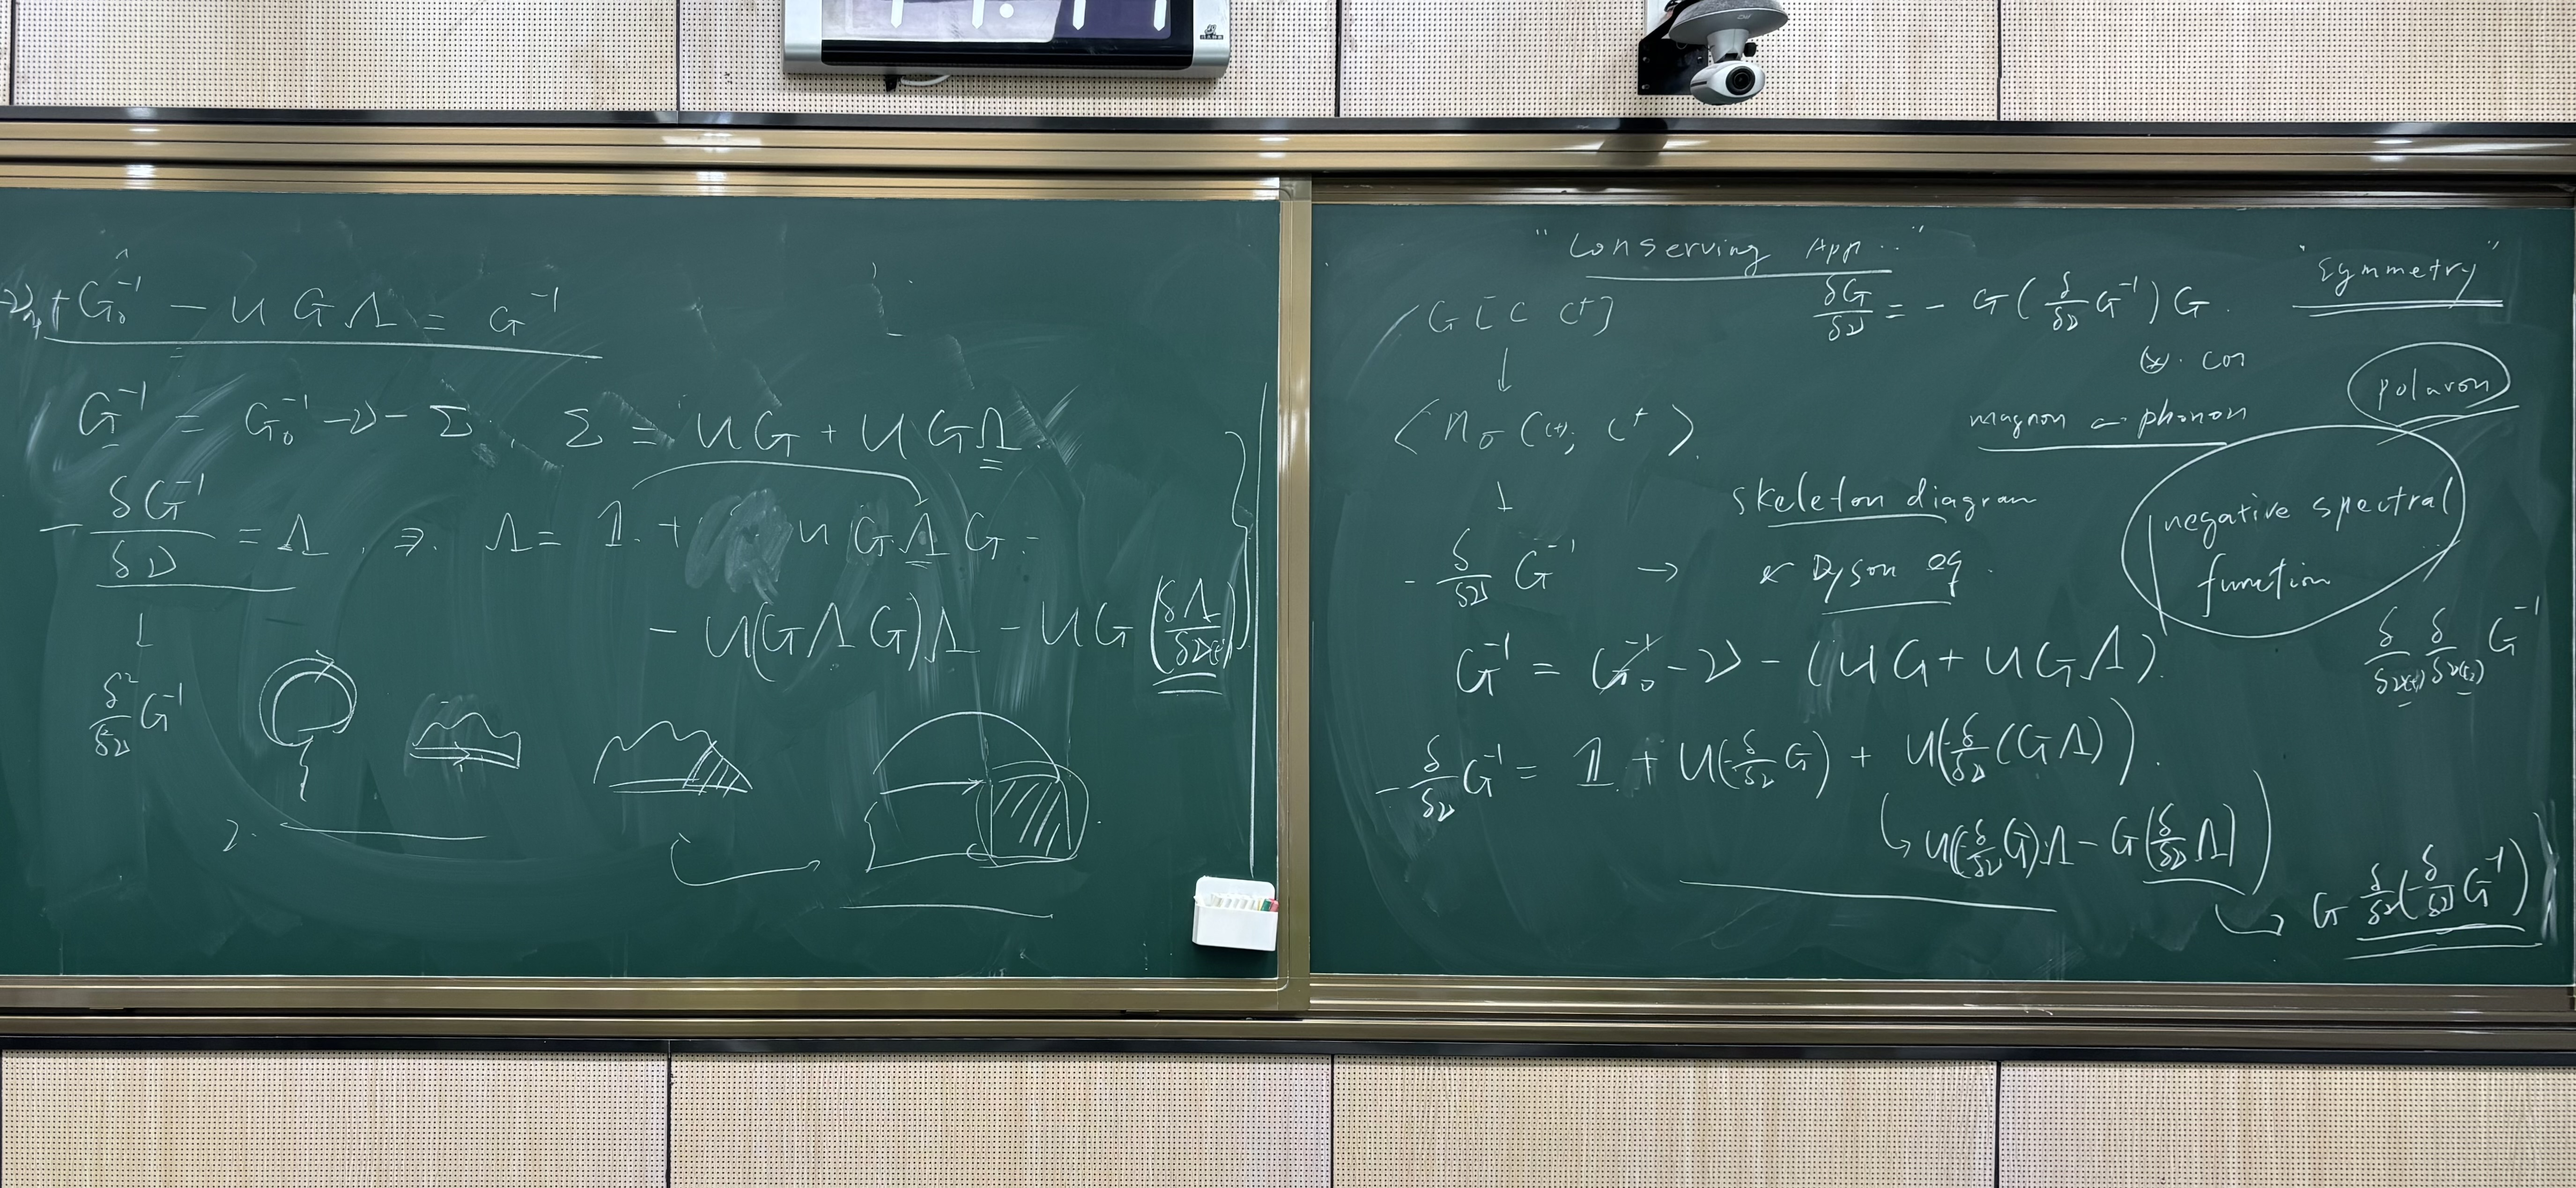
\includegraphics[width = \linewidth]{./media/feynmann28.jpeg}
\end{center}
Also: Negative spectral, magnon \texttt{<->} phonon, Ploavon.

Very important is to apply symmetry to pertubation theory:
Conserving application.

\paragraph{Fermi liquid}

\begin{center}
  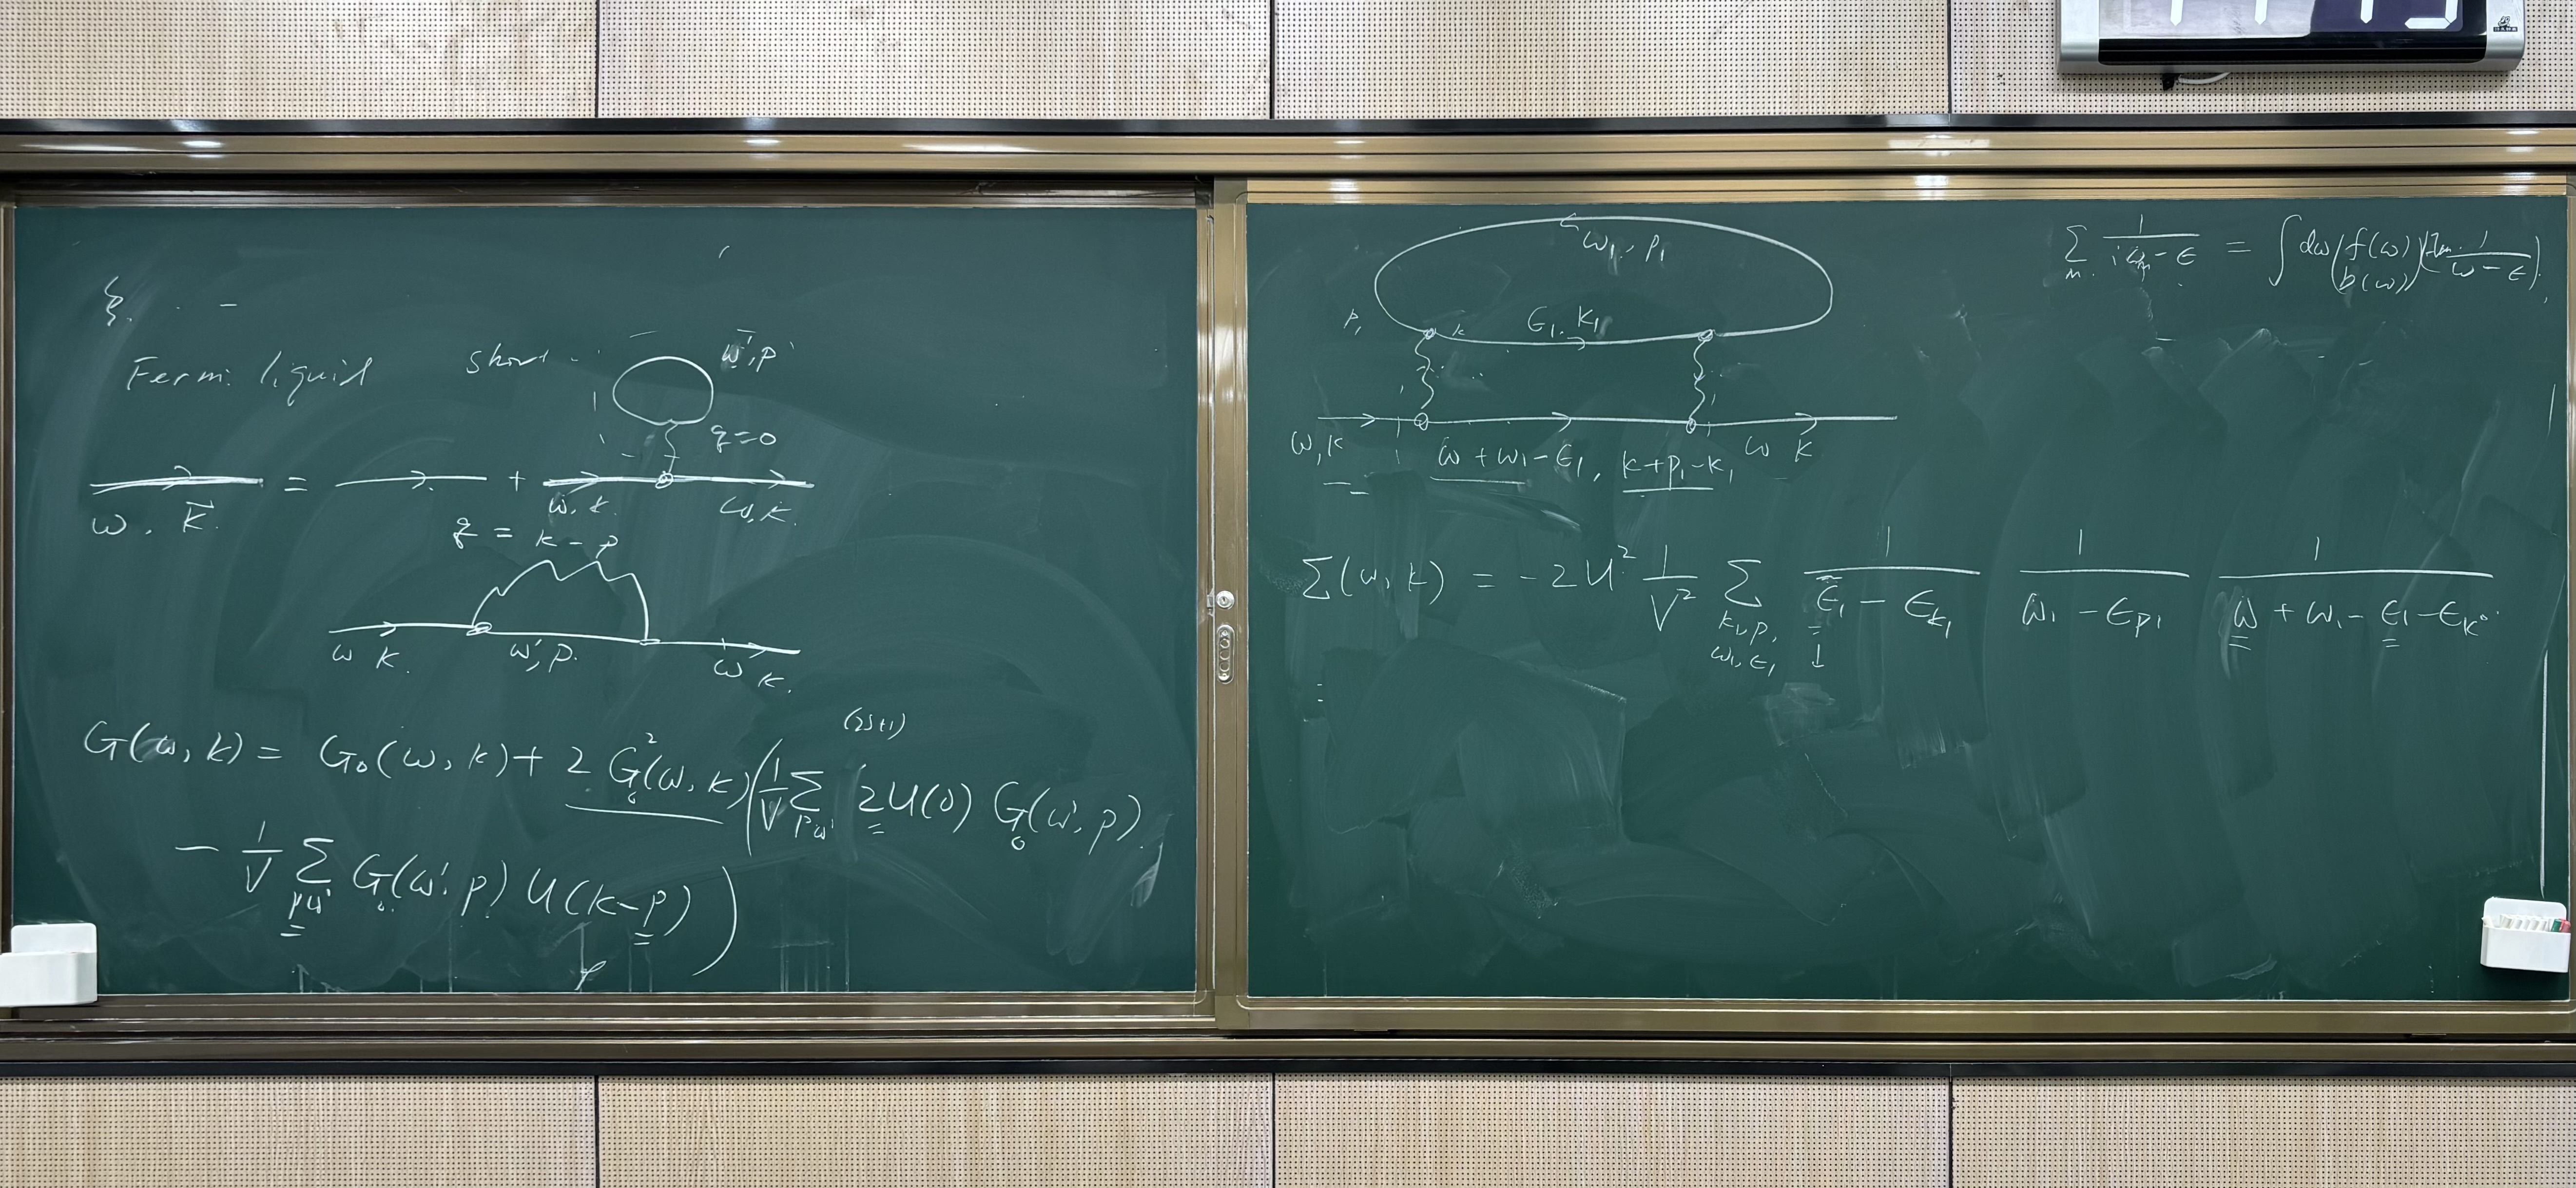
\includegraphics[width = \linewidth]{./media/feynmann29.jpeg}
\end{center}
\[
  G(\omega, k) = G_0(\omega, k) + 2G^2(\omega, k)
    \ab(\frac1V \sum_{p\omega}) 2U(0) G(\omega',p)
    - \frac1V \sum_{pu^2} G(\omega', p) U(k - p)
\]
The self energy
\begin{multline*}
  \Sigma(\omega, k) = -2U^2\frac1{V^2}
    \sum_{\substack{k_1, p\\\omega_1,\epsilon_1}}
  \frac1{\tilde \epsilon_1 - \epsilon_{k_1}}
  \frac1{\omega_1 - \epsilon_{p_1}}
  \frac1{\omega + \omega_1 - \epsilon_1 - \epsilon_{k^0}}\\
= \frac{2U^2}{V^2} \sum_{k_0, k_1, p} \delta_{k+1_0} \delta_{k+p_1}
  \frac1{\omega + \epsilon_{p_1} - \epsilon_{p_0} - \epsilon_{k_1}}
  (1 - f(\epsilon_1) - f(\epsilon_{k_0}))
\end{multline*}
where $(f(\epsilon_{p_1} + b(\epsilon_{k_0} + \epsilon_{k_1})))$,
$b(x + y) = \frac{f(x)f(y)}{1- f(x) - f(y)}$, and we can take
\[
  \Delta\omega = \omega_1 - \epsilon_1, \quad
  \Delta p = p_1 - k_1.
\]
At finite temperatore, we can convert
\[
  \sum_\mu \frac1{\iu c_\mu - \epsilon}
= \int \omega (f(\omega) \qq{or} b(\omega)) \cdot \frac1{\omega - \epsilon}
\]
To sum
\begin{align*}
  \sum_{\epsilon_1} \frac1{\epsilon_1 - \epsilon_{k_1}}
    \frac1{\omega + \omega_1 - \epsilon_1 - \epsilon_{k_0}}
& = \int \d\epsilon_1 [f(\epsilon_{k_1} \delta(\epsilon_1 - \epsilon_{k_1})
    - (1 - f(\epsilon_{k_1}) \delta(\epsilon_1 - \epsilon_{k_1})))]
  \frac1{\omega + \omega_1 - \epsilon_1 - \epsilon_{k_0}}\\
& = \frac{f(\epsilon_{k_1})}{\omega + \omega_1 - \epsilon_1 - \epsilon_{k_0}}
  - \frac{1 - f(\epsilon_{k_1})}
      {\omega + \omega_1 - \epsilon_1 - \epsilon_{k_0}}
\end{align*}
where
\[
  \frac1{(\epsilon_1 - \epsilon_{k_1})
    (\omega + \omega_1 - \epsilon_1 - \epsilon_{k_0})}
= \ab(\frac 1{\epsilon_1 - \epsilon_{k_1}}
+ \frac 1{\omega + \omega_1 - \epsilon_1 - \epsilon_{k_0}})
  \frac1{\omega + \omega_1 - \epsilon_{k_0} - \epsilon_{k_1}}
\]
where $\frac 1{\omega + \omega_1 - \epsilon_1 - \epsilon_{k_0}}$ get
$f(\omega + \omega_1 - \epsilon_1)$.
Finally,
\[
  \sum_{\epsilon_1} \frac1{\epsilon_1 - \epsilon_{k_1}}
    \frac1{\omega + \omega_1 - \epsilon_1 - \epsilon_{k_0}}
= -(1 - f(\epsilon_{k_1})) = f(\epsilon_{k_0})
    \frac1{\omega + \omega_1 - \epsilon_{k_0} - \epsilon_{k_1}}
\]
Three momentums become three energy
\begin{multline*}
  \Im \Sigma(\omega, k) = -2\pi u^2 \rho_0^3 \int_0^\epsilon
    \d\epsilon_0 \d\epsilon_1 \d\omega_1 S_k(\epsilon_0, \epsilon_1, \omega_1)
    \delta(\epsilon - \omega_1 - \epsilon_1 - \epsilon_0)
    (f(\omega_1) (1 - f(\epsilon_0))(1 - f(\epsilon_1)))\\
    + (1 - f(\omega_0)) f(\epsilon_0) f(\epsilon_1)
  \xlongequal{\epsilon \ll \epsilon_F}
  -2\pi u^2 \rho_0^3 S_k(0,0,0) (\epsilon^2 + T^2)/2
\end{multline*}
Then
\[
  S_k(\epsilon_0, \epsilon_1, \omega_1)
= \frac1{\rho_0^3} \frac1{V^2} \sum_{k_0k_1\beta_1}
  \delta(\epsilon_0 - \epsilon_{k_0})
  \delta(\epsilon_1 - \epsilon_{k_1}) \delta(\omega_1 - \epsilon_{p_0})
  \delta_{k+p_1, k_0+k_1}
\]
So, the self-energy
\[
  \lim_{\substack{\epsilon\to0\\k\to0}}
  \Im \Sigma(\epsilon, k) \sim
  \begin{cases}
    \epsilon^2, & d = 3,\\
    \epsilon^2 \ln|\epsilon| \big|_{\epsilon \to 0 } \to 0, & d = 2,\\
    -|\epsilon| \to \pdv\Sigma\epsilon\bigg|_{\epsilon \to -} \to \infty, &
      d = 1
  \end{cases}
\]
For 1D, we will have Luttinger liquid $z = 0$.
The occupation number $f(k)$. The quasi-particle weight $Z$.
The first derivative of $f(k)$ to $k$ would be continuous.